\documentclass[twoside]{book}

% Packages required by doxygen
\usepackage{fixltx2e}
\usepackage{calc}
\usepackage{doxygen}
\usepackage{graphicx}
\usepackage[utf8]{inputenc}
\usepackage{makeidx}
\usepackage{multicol}
\usepackage{multirow}
\PassOptionsToPackage{warn}{textcomp}
\usepackage{textcomp}
\usepackage[nointegrals]{wasysym}
\usepackage[table]{xcolor}

% Font selection
\usepackage[T1]{fontenc}
\usepackage{mathptmx}
\usepackage[scaled=.90]{helvet}
\usepackage{courier}
\usepackage{amssymb}
\usepackage{sectsty}
\renewcommand{\familydefault}{\sfdefault}
\allsectionsfont{%
  \fontseries{bc}\selectfont%
  \color{darkgray}%
}
\renewcommand{\DoxyLabelFont}{%
  \fontseries{bc}\selectfont%
  \color{darkgray}%
}
\newcommand{\+}{\discretionary{\mbox{\scriptsize$\hookleftarrow$}}{}{}}

% Page & text layout
\usepackage{geometry}
\geometry{%
  a4paper,%
  top=2.5cm,%
  bottom=2.5cm,%
  left=2.5cm,%
  right=2.5cm%
}
\tolerance=750
\hfuzz=15pt
\hbadness=750
\setlength{\emergencystretch}{15pt}
\setlength{\parindent}{0cm}
\setlength{\parskip}{0.2cm}
\makeatletter
\renewcommand{\paragraph}{%
  \@startsection{paragraph}{4}{0ex}{-1.0ex}{1.0ex}{%
    \normalfont\normalsize\bfseries\SS@parafont%
  }%
}
\renewcommand{\subparagraph}{%
  \@startsection{subparagraph}{5}{0ex}{-1.0ex}{1.0ex}{%
    \normalfont\normalsize\bfseries\SS@subparafont%
  }%
}
\makeatother

% Headers & footers
\usepackage{fancyhdr}
\pagestyle{fancyplain}
\fancyhead[LE]{\fancyplain{}{\bfseries\thepage}}
\fancyhead[CE]{\fancyplain{}{}}
\fancyhead[RE]{\fancyplain{}{\bfseries\leftmark}}
\fancyhead[LO]{\fancyplain{}{\bfseries\rightmark}}
\fancyhead[CO]{\fancyplain{}{}}
\fancyhead[RO]{\fancyplain{}{\bfseries\thepage}}
\fancyfoot[LE]{\fancyplain{}{}}
\fancyfoot[CE]{\fancyplain{}{}}
\fancyfoot[RE]{\fancyplain{}{\bfseries\scriptsize Generated on Wed Nov 19 2014 16\+:58\+:14 for Stand\+Alone\+Framework by Doxygen }}
\fancyfoot[LO]{\fancyplain{}{\bfseries\scriptsize Generated on Wed Nov 19 2014 16\+:58\+:14 for Stand\+Alone\+Framework by Doxygen }}
\fancyfoot[CO]{\fancyplain{}{}}
\fancyfoot[RO]{\fancyplain{}{}}
\renewcommand{\footrulewidth}{0.4pt}
\renewcommand{\chaptermark}[1]{%
  \markboth{#1}{}%
}
\renewcommand{\sectionmark}[1]{%
  \markright{\thesection\ #1}%
}

% Indices & bibliography
\usepackage{natbib}
\usepackage[titles]{tocloft}
\setcounter{tocdepth}{3}
\setcounter{secnumdepth}{5}
\makeindex

% Hyperlinks (required, but should be loaded last)
\usepackage{ifpdf}
\ifpdf
  \usepackage[pdftex,pagebackref=true]{hyperref}
\else
  \usepackage[ps2pdf,pagebackref=true]{hyperref}
\fi
\hypersetup{%
  colorlinks=true,%
  linkcolor=blue,%
  citecolor=blue,%
  unicode%
}

% Custom commands
\newcommand{\clearemptydoublepage}{%
  \newpage{\pagestyle{empty}\cleardoublepage}%
}


%===== C O N T E N T S =====

\begin{document}

% Titlepage & ToC
\hypersetup{pageanchor=false,
             bookmarks=true,
             bookmarksnumbered=true,
             pdfencoding=unicode
            }
\pagenumbering{roman}
\begin{titlepage}
\vspace*{7cm}
\begin{center}%
{\Large Stand\+Alone\+Framework \\[1ex]\large 1.\+0.\+0 }\\
\vspace*{1cm}
{\large Generated by Doxygen 1.8.8}\\
\vspace*{0.5cm}
{\small Wed Nov 19 2014 16:58:14}\\
\end{center}
\end{titlepage}
\clearemptydoublepage
\tableofcontents
\clearemptydoublepage
\pagenumbering{arabic}
\hypersetup{pageanchor=true}

%--- Begin generated contents ---
\chapter{Namespace Index}
\section{Packages}
Here are the packages with brief descriptions (if available)\+:\begin{DoxyCompactList}
\item\contentsline{section}{\hyperlink{namespace_stand_alone_framework}{Stand\+Alone\+Framework} }{\pageref{namespace_stand_alone_framework}}{}
\item\contentsline{section}{\hyperlink{namespace_stand_alone_framework_1_1_extensions}{Stand\+Alone\+Framework.\+Extensions} }{\pageref{namespace_stand_alone_framework_1_1_extensions}}{}
\item\contentsline{section}{\hyperlink{namespace_stand_alone_framework_1_1_factories}{Stand\+Alone\+Framework.\+Factories} }{\pageref{namespace_stand_alone_framework_1_1_factories}}{}
\item\contentsline{section}{\hyperlink{namespace_stand_alone_framework_1_1_factories_1_1_interfaces}{Stand\+Alone\+Framework.\+Factories.\+Interfaces} }{\pageref{namespace_stand_alone_framework_1_1_factories_1_1_interfaces}}{}
\item\contentsline{section}{\hyperlink{namespace_stand_alone_framework_1_1_factories_1_1_method_factory}{Stand\+Alone\+Framework.\+Factories.\+Method\+Factory} }{\pageref{namespace_stand_alone_framework_1_1_factories_1_1_method_factory}}{}
\item\contentsline{section}{\hyperlink{namespace_stand_alone_framework_1_1_factories_1_1_thread_factory}{Stand\+Alone\+Framework.\+Factories.\+Thread\+Factory} }{\pageref{namespace_stand_alone_framework_1_1_factories_1_1_thread_factory}}{}
\item\contentsline{section}{\hyperlink{namespace_stand_alone_framework_1_1_framework_classes}{Stand\+Alone\+Framework.\+Framework\+Classes} }{\pageref{namespace_stand_alone_framework_1_1_framework_classes}}{}
\item\contentsline{section}{\hyperlink{namespace_stand_alone_framework_1_1_intefaces}{Stand\+Alone\+Framework.\+Intefaces} }{\pageref{namespace_stand_alone_framework_1_1_intefaces}}{}
\item\contentsline{section}{\hyperlink{namespace_stand_alone_framework_1_1_interfaces}{Stand\+Alone\+Framework.\+Interfaces} }{\pageref{namespace_stand_alone_framework_1_1_interfaces}}{}
\item\contentsline{section}{\hyperlink{namespace_stand_alone_framework_1_1_method_facade}{Stand\+Alone\+Framework.\+Method\+Facade} }{\pageref{namespace_stand_alone_framework_1_1_method_facade}}{}
\item\contentsline{section}{\hyperlink{namespace_stand_alone_framework_1_1_method_facade_1_1_interfaces}{Stand\+Alone\+Framework.\+Method\+Facade.\+Interfaces} }{\pageref{namespace_stand_alone_framework_1_1_method_facade_1_1_interfaces}}{}
\item\contentsline{section}{\hyperlink{namespace_stand_alone_framework_test}{Stand\+Alone\+Framework\+Test} }{\pageref{namespace_stand_alone_framework_test}}{}
\item\contentsline{section}{\hyperlink{namespace_stand_alone_framework_test_1_1_stateful_tests}{Stand\+Alone\+Framework\+Test.\+Stateful\+Tests} }{\pageref{namespace_stand_alone_framework_test_1_1_stateful_tests}}{}
\item\contentsline{section}{\hyperlink{namespace_stand_alone_framework_test_1_1_stateful_tests_1_1_cache_manager}{Stand\+Alone\+Framework\+Test.\+Stateful\+Tests.\+Cache\+Manager} }{\pageref{namespace_stand_alone_framework_test_1_1_stateful_tests_1_1_cache_manager}}{}
\end{DoxyCompactList}

\chapter{Hierarchical Index}
\section{Class Hierarchy}
This inheritance list is sorted roughly, but not completely, alphabetically\+:\begin{DoxyCompactList}
\item \contentsline{section}{Stand\+Alone\+Framework\+Test.\+Stateful\+Tests.\+Cache\+Manager.\+Cache\+Manger\+Test\+Fixture}{\pageref{class_stand_alone_framework_test_1_1_stateful_tests_1_1_cache_manager_1_1_cache_manger_test_fixture}}{}
\item \contentsline{section}{Stand\+Alone\+Framework.\+Code\+Contract\+Validator}{\pageref{class_stand_alone_framework_1_1_code_contract_validator}}{}
\item \contentsline{section}{Stand\+Alone\+Framework.\+Data\+Wrapper}{\pageref{class_stand_alone_framework_1_1_data_wrapper}}{}
\item \contentsline{section}{Stand\+Alone\+Framework.\+Interfaces.\+I\+Cache\+Manager$<$ T $>$}{\pageref{interface_stand_alone_framework_1_1_interfaces_1_1_i_cache_manager_3_01_t_01_4}}{}
\begin{DoxyCompactList}
\item \contentsline{section}{Stand\+Alone\+Framework.\+Cache\+Manager$<$ T $>$}{\pageref{class_stand_alone_framework_1_1_cache_manager_3_01_t_01_4}}{}
\end{DoxyCompactList}
\item I\+Disposable\begin{DoxyCompactList}
\item \contentsline{section}{Stand\+Alone\+Framework.\+Memory\+Manager$<$ T $>$}{\pageref{class_stand_alone_framework_1_1_memory_manager_3_01_t_01_4}}{}
\begin{DoxyCompactList}
\item \contentsline{section}{Stand\+Alone\+Framework.\+Framework\+Classes.\+Invocation\+Result}{\pageref{class_stand_alone_framework_1_1_framework_classes_1_1_invocation_result}}{}
\end{DoxyCompactList}
\end{DoxyCompactList}
\item \contentsline{section}{Stand\+Alone\+Framework.\+Intefaces.\+I\+Dynamic\+Invoker}{\pageref{interface_stand_alone_framework_1_1_intefaces_1_1_i_dynamic_invoker}}{}
\begin{DoxyCompactList}
\item \contentsline{section}{Stand\+Alone\+Framework.\+Dyamic\+Invoker}{\pageref{class_stand_alone_framework_1_1_dyamic_invoker}}{}
\end{DoxyCompactList}
\item \contentsline{section}{Stand\+Alone\+Framework.\+Interfaces.\+I\+Error\+Manager}{\pageref{interface_stand_alone_framework_1_1_interfaces_1_1_i_error_manager}}{}
\begin{DoxyCompactList}
\item \contentsline{section}{Stand\+Alone\+Framework.\+Error\+Manager}{\pageref{class_stand_alone_framework_1_1_error_manager}}{}
\begin{DoxyCompactList}
\item \contentsline{section}{Stand\+Alone\+Framework.\+Dyamic\+Invoker}{\pageref{class_stand_alone_framework_1_1_dyamic_invoker}}{}
\end{DoxyCompactList}
\end{DoxyCompactList}
\item \contentsline{section}{Stand\+Alone\+Framework.\+Interfaces.\+I\+Memory\+Manager}{\pageref{interface_stand_alone_framework_1_1_interfaces_1_1_i_memory_manager}}{}
\begin{DoxyCompactList}
\item \contentsline{section}{Stand\+Alone\+Framework.\+Memory\+Manager$<$ T $>$}{\pageref{class_stand_alone_framework_1_1_memory_manager_3_01_t_01_4}}{}
\end{DoxyCompactList}
\item \contentsline{section}{Stand\+Alone\+Framework.\+Interfaces.\+I\+Message\+Handler}{\pageref{interface_stand_alone_framework_1_1_interfaces_1_1_i_message_handler}}{}
\begin{DoxyCompactList}
\item \contentsline{section}{Stand\+Alone\+Framework.\+Message\+Handler}{\pageref{class_stand_alone_framework_1_1_message_handler}}{}
\begin{DoxyCompactList}
\item \contentsline{section}{Stand\+Alone\+Framework.\+Error\+Manager}{\pageref{class_stand_alone_framework_1_1_error_manager}}{}
\end{DoxyCompactList}
\end{DoxyCompactList}
\item \contentsline{section}{Stand\+Alone\+Framework.\+Method\+Facade.\+Interfaces.\+I\+Method\+Facade}{\pageref{interface_stand_alone_framework_1_1_method_facade_1_1_interfaces_1_1_i_method_facade}}{}
\begin{DoxyCompactList}
\item \contentsline{section}{Stand\+Alone\+Framework.\+Method\+Facade.\+Method\+Facade}{\pageref{class_stand_alone_framework_1_1_method_facade_1_1_method_facade}}{}
\end{DoxyCompactList}
\item \contentsline{section}{Stand\+Alone\+Framework.\+Factories.\+Interfaces.\+I\+Method\+Factory}{\pageref{interface_stand_alone_framework_1_1_factories_1_1_interfaces_1_1_i_method_factory}}{}
\begin{DoxyCompactList}
\item \contentsline{section}{Stand\+Alone\+Framework.\+Factories.\+Method\+Factory.\+Method\+Factory}{\pageref{class_stand_alone_framework_1_1_factories_1_1_method_factory_1_1_method_factory}}{}
\end{DoxyCompactList}
\item \contentsline{section}{Stand\+Alone\+Framework.\+Factories.\+Interfaces.\+I\+Thread\+Factory}{\pageref{interface_stand_alone_framework_1_1_factories_1_1_interfaces_1_1_i_thread_factory}}{}
\begin{DoxyCompactList}
\item \contentsline{section}{Stand\+Alone\+Framework.\+Factories.\+Thread\+Factory.\+Thread\+Factory}{\pageref{class_stand_alone_framework_1_1_factories_1_1_thread_factory_1_1_thread_factory}}{}
\end{DoxyCompactList}
\item \contentsline{section}{Stand\+Alone\+Framework.\+Factories.\+Method\+Factory.\+Method\+Wrapper}{\pageref{class_stand_alone_framework_1_1_factories_1_1_method_factory_1_1_method_wrapper}}{}
\item \contentsline{section}{Stand\+Alone\+Framework\+Test.\+Stateful\+Tests.\+Cache\+Manager.\+Person}{\pageref{class_stand_alone_framework_test_1_1_stateful_tests_1_1_cache_manager_1_1_person}}{}
\end{DoxyCompactList}

\chapter{Class Index}
\section{Class List}
Here are the classes, structs, unions and interfaces with brief descriptions\+:\begin{DoxyCompactList}
\item\contentsline{section}{\hyperlink{class_stand_alone_framework_1_1_cache_manager_3_01_t_01_4}{Stand\+Alone\+Framework.\+Cache\+Manager$<$ T $>$} \\*Acts as a central store for all objects who need to be cached }{\pageref{class_stand_alone_framework_1_1_cache_manager_3_01_t_01_4}}{}
\item\contentsline{section}{\hyperlink{class_stand_alone_framework_test_1_1_stateful_tests_1_1_cache_manager_1_1_cache_manger_test_fixture}{Stand\+Alone\+Framework\+Test.\+Stateful\+Tests.\+Cache\+Manager.\+Cache\+Manger\+Test\+Fixture} }{\pageref{class_stand_alone_framework_test_1_1_stateful_tests_1_1_cache_manager_1_1_cache_manger_test_fixture}}{}
\item\contentsline{section}{\hyperlink{class_stand_alone_framework_1_1_code_contract_validator}{Stand\+Alone\+Framework.\+Code\+Contract\+Validator} \\*Acts as a code contract validator. This is needed to ensure that all contracts conditions are met prior to any code execution }{\pageref{class_stand_alone_framework_1_1_code_contract_validator}}{}
\item\contentsline{section}{\hyperlink{class_stand_alone_framework_1_1_data_wrapper}{Stand\+Alone\+Framework.\+Data\+Wrapper} \\*Acts as a wrapper for the arguments that need to be passed into the method }{\pageref{class_stand_alone_framework_1_1_data_wrapper}}{}
\item\contentsline{section}{\hyperlink{class_stand_alone_framework_1_1_dyamic_invoker}{Stand\+Alone\+Framework.\+Dyamic\+Invoker} \\*Represents a class that is able to execute a method without knowing the internal workings. It also wraps the method call in an error handler and defers all error handling the the {\ttfamily \hyperlink{class_stand_alone_framework_1_1_error_manager}{Error\+Manager} class} }{\pageref{class_stand_alone_framework_1_1_dyamic_invoker}}{}
\item\contentsline{section}{\hyperlink{class_stand_alone_framework_1_1_error_manager}{Stand\+Alone\+Framework.\+Error\+Manager} \\*Acts as the central error handling component during method execution. }{\pageref{class_stand_alone_framework_1_1_error_manager}}{}
\item\contentsline{section}{\hyperlink{interface_stand_alone_framework_1_1_interfaces_1_1_i_cache_manager_3_01_t_01_4}{Stand\+Alone\+Framework.\+Interfaces.\+I\+Cache\+Manager$<$ T $>$} \\*The Cache\+Manager's contract }{\pageref{interface_stand_alone_framework_1_1_interfaces_1_1_i_cache_manager_3_01_t_01_4}}{}
\item\contentsline{section}{\hyperlink{interface_stand_alone_framework_1_1_intefaces_1_1_i_dynamic_invoker}{Stand\+Alone\+Framework.\+Intefaces.\+I\+Dynamic\+Invoker} \\*The Dynamic\+Invokers contract }{\pageref{interface_stand_alone_framework_1_1_intefaces_1_1_i_dynamic_invoker}}{}
\item\contentsline{section}{\hyperlink{interface_stand_alone_framework_1_1_interfaces_1_1_i_error_manager}{Stand\+Alone\+Framework.\+Interfaces.\+I\+Error\+Manager} \\*The \hyperlink{class_stand_alone_framework_1_1_error_manager}{Error\+Manager} contract }{\pageref{interface_stand_alone_framework_1_1_interfaces_1_1_i_error_manager}}{}
\item\contentsline{section}{\hyperlink{interface_stand_alone_framework_1_1_interfaces_1_1_i_memory_manager}{Stand\+Alone\+Framework.\+Interfaces.\+I\+Memory\+Manager} }{\pageref{interface_stand_alone_framework_1_1_interfaces_1_1_i_memory_manager}}{}
\item\contentsline{section}{\hyperlink{interface_stand_alone_framework_1_1_interfaces_1_1_i_message_handler}{Stand\+Alone\+Framework.\+Interfaces.\+I\+Message\+Handler} }{\pageref{interface_stand_alone_framework_1_1_interfaces_1_1_i_message_handler}}{}
\item\contentsline{section}{\hyperlink{interface_stand_alone_framework_1_1_method_facade_1_1_interfaces_1_1_i_method_facade}{Stand\+Alone\+Framework.\+Method\+Facade.\+Interfaces.\+I\+Method\+Facade} \\*The \hyperlink{class_stand_alone_framework_1_1_method_facade_1_1_method_facade}{Method\+Facade} contract }{\pageref{interface_stand_alone_framework_1_1_method_facade_1_1_interfaces_1_1_i_method_facade}}{}
\item\contentsline{section}{\hyperlink{interface_stand_alone_framework_1_1_factories_1_1_interfaces_1_1_i_method_factory}{Stand\+Alone\+Framework.\+Factories.\+Interfaces.\+I\+Method\+Factory} }{\pageref{interface_stand_alone_framework_1_1_factories_1_1_interfaces_1_1_i_method_factory}}{}
\item\contentsline{section}{\hyperlink{class_stand_alone_framework_1_1_framework_classes_1_1_invocation_result}{Stand\+Alone\+Framework.\+Framework\+Classes.\+Invocation\+Result} \\*Encapsulates the return values of the method execution. The return values could contain contain any error messages, data that is returned from the method execution }{\pageref{class_stand_alone_framework_1_1_framework_classes_1_1_invocation_result}}{}
\item\contentsline{section}{\hyperlink{interface_stand_alone_framework_1_1_factories_1_1_interfaces_1_1_i_thread_factory}{Stand\+Alone\+Framework.\+Factories.\+Interfaces.\+I\+Thread\+Factory} \\*The \hyperlink{namespace_stand_alone_framework_1_1_factories_1_1_thread_factory}{Thread\+Factory} contract }{\pageref{interface_stand_alone_framework_1_1_factories_1_1_interfaces_1_1_i_thread_factory}}{}
\item\contentsline{section}{\hyperlink{class_stand_alone_framework_1_1_memory_manager_3_01_t_01_4}{Stand\+Alone\+Framework.\+Memory\+Manager$<$ T $>$} \\*Represents the memory manager that active manages the lifetime of any object that derives from it }{\pageref{class_stand_alone_framework_1_1_memory_manager_3_01_t_01_4}}{}
\item\contentsline{section}{\hyperlink{class_stand_alone_framework_1_1_message_handler}{Stand\+Alone\+Framework.\+Message\+Handler} \\*Acts as a central message handler. This would defer all the message displaying functionality to either the front end, or could be used together M\+S\+M\+Q }{\pageref{class_stand_alone_framework_1_1_message_handler}}{}
\item\contentsline{section}{\hyperlink{class_stand_alone_framework_1_1_method_facade_1_1_method_facade}{Stand\+Alone\+Framework.\+Method\+Facade.\+Method\+Facade} \\*Represents the facade or entry point of all method calls into the framework }{\pageref{class_stand_alone_framework_1_1_method_facade_1_1_method_facade}}{}
\item\contentsline{section}{\hyperlink{class_stand_alone_framework_1_1_factories_1_1_method_factory_1_1_method_factory}{Stand\+Alone\+Framework.\+Factories.\+Method\+Factory.\+Method\+Factory} \\*Encapsulates functionality that creates and wraps a method with a thread as well as any arguments that the method requires. }{\pageref{class_stand_alone_framework_1_1_factories_1_1_method_factory_1_1_method_factory}}{}
\item\contentsline{section}{\hyperlink{class_stand_alone_framework_1_1_factories_1_1_method_factory_1_1_method_wrapper}{Stand\+Alone\+Framework.\+Factories.\+Method\+Factory.\+Method\+Wrapper} \\*Class \hyperlink{class_stand_alone_framework_1_1_factories_1_1_method_factory_1_1_method_wrapper}{Method\+Wrapper} }{\pageref{class_stand_alone_framework_1_1_factories_1_1_method_factory_1_1_method_wrapper}}{}
\item\contentsline{section}{\hyperlink{class_stand_alone_framework_test_1_1_stateful_tests_1_1_cache_manager_1_1_person}{Stand\+Alone\+Framework\+Test.\+Stateful\+Tests.\+Cache\+Manager.\+Person} }{\pageref{class_stand_alone_framework_test_1_1_stateful_tests_1_1_cache_manager_1_1_person}}{}
\item\contentsline{section}{\hyperlink{class_stand_alone_framework_1_1_factories_1_1_thread_factory_1_1_thread_factory}{Stand\+Alone\+Framework.\+Factories.\+Thread\+Factory.\+Thread\+Factory} \\*Represents a factory that creates, terminates and handles any thread related tasks for the current method execution }{\pageref{class_stand_alone_framework_1_1_factories_1_1_thread_factory_1_1_thread_factory}}{}
\end{DoxyCompactList}

\chapter{File Index}
\section{File List}
Here is a list of all files with brief descriptions\+:\begin{DoxyCompactList}
\item\contentsline{section}{C\+:/\+Users/\+Charles Trent Spare/\+Documents/\+Source Control/\+Repositories/\+Development\+Projects/\+Stand\+Alone\+Framework/\+Stand\+Alone\+Framework/\hyperlink{_data_wrapper_8cs}{Data\+Wrapper.\+cs} }{\pageref{_data_wrapper_8cs}}{}
\item\contentsline{section}{C\+:/\+Users/\+Charles Trent Spare/\+Documents/\+Source Control/\+Repositories/\+Development\+Projects/\+Stand\+Alone\+Framework/\+Stand\+Alone\+Framework/\+Cache\+Manager/\hyperlink{_cache_manager_8cs}{Cache\+Manager.\+cs} }{\pageref{_cache_manager_8cs}}{}
\item\contentsline{section}{C\+:/\+Users/\+Charles Trent Spare/\+Documents/\+Source Control/\+Repositories/\+Development\+Projects/\+Stand\+Alone\+Framework/\+Stand\+Alone\+Framework/\+Cache\+Manager/\+Interfaces/\hyperlink{_i_cache_manager_8cs}{I\+Cache\+Manager.\+cs} }{\pageref{_i_cache_manager_8cs}}{}
\item\contentsline{section}{C\+:/\+Users/\+Charles Trent Spare/\+Documents/\+Source Control/\+Repositories/\+Development\+Projects/\+Stand\+Alone\+Framework/\+Stand\+Alone\+Framework/\+Code\+Contract\+Validator/\hyperlink{_code_contract_validator_8cs}{Code\+Contract\+Validator.\+cs} }{\pageref{_code_contract_validator_8cs}}{}
\item\contentsline{section}{C\+:/\+Users/\+Charles Trent Spare/\+Documents/\+Source Control/\+Repositories/\+Development\+Projects/\+Stand\+Alone\+Framework/\+Stand\+Alone\+Framework/\+Dynamic\+Invoker/\hyperlink{_dyamic_invoker_8cs}{Dyamic\+Invoker.\+cs} }{\pageref{_dyamic_invoker_8cs}}{}
\item\contentsline{section}{C\+:/\+Users/\+Charles Trent Spare/\+Documents/\+Source Control/\+Repositories/\+Development\+Projects/\+Stand\+Alone\+Framework/\+Stand\+Alone\+Framework/\+Dynamic\+Invoker/\+Intefaces/\hyperlink{_i_dynamic_invoker_8cs}{I\+Dynamic\+Invoker.\+cs} }{\pageref{_i_dynamic_invoker_8cs}}{}
\item\contentsline{section}{C\+:/\+Users/\+Charles Trent Spare/\+Documents/\+Source Control/\+Repositories/\+Development\+Projects/\+Stand\+Alone\+Framework/\+Stand\+Alone\+Framework/\+Error\+Manager/\hyperlink{_error_manager_8cs}{Error\+Manager.\+cs} }{\pageref{_error_manager_8cs}}{}
\item\contentsline{section}{C\+:/\+Users/\+Charles Trent Spare/\+Documents/\+Source Control/\+Repositories/\+Development\+Projects/\+Stand\+Alone\+Framework/\+Stand\+Alone\+Framework/\+Error\+Manager/\+Interfaces/\hyperlink{_i_error_manager_8cs}{I\+Error\+Manager.\+cs} }{\pageref{_i_error_manager_8cs}}{}
\item\contentsline{section}{C\+:/\+Users/\+Charles Trent Spare/\+Documents/\+Source Control/\+Repositories/\+Development\+Projects/\+Stand\+Alone\+Framework/\+Stand\+Alone\+Framework/\+Extensions/\hyperlink{_collection_extensions_8cs}{Collection\+Extensions.\+cs} }{\pageref{_collection_extensions_8cs}}{}
\item\contentsline{section}{C\+:/\+Users/\+Charles Trent Spare/\+Documents/\+Source Control/\+Repositories/\+Development\+Projects/\+Stand\+Alone\+Framework/\+Stand\+Alone\+Framework/\+Extensions/\hyperlink{_faux_extensions_8cs}{Faux\+Extensions.\+cs} }{\pageref{_faux_extensions_8cs}}{}
\item\contentsline{section}{C\+:/\+Users/\+Charles Trent Spare/\+Documents/\+Source Control/\+Repositories/\+Development\+Projects/\+Stand\+Alone\+Framework/\+Stand\+Alone\+Framework/\+Extensions/\hyperlink{_object_extensions_8cs}{Object\+Extensions.\+cs} }{\pageref{_object_extensions_8cs}}{}
\item\contentsline{section}{C\+:/\+Users/\+Charles Trent Spare/\+Documents/\+Source Control/\+Repositories/\+Development\+Projects/\+Stand\+Alone\+Framework/\+Stand\+Alone\+Framework/\+Extensions/\hyperlink{_string_extensions_8cs}{String\+Extensions.\+cs} }{\pageref{_string_extensions_8cs}}{}
\item\contentsline{section}{C\+:/\+Users/\+Charles Trent Spare/\+Documents/\+Source Control/\+Repositories/\+Development\+Projects/\+Stand\+Alone\+Framework/\+Stand\+Alone\+Framework/\+Factories/\+Method\+Factory/\hyperlink{_method_factory_8cs}{Method\+Factory.\+cs} }{\pageref{_method_factory_8cs}}{}
\item\contentsline{section}{C\+:/\+Users/\+Charles Trent Spare/\+Documents/\+Source Control/\+Repositories/\+Development\+Projects/\+Stand\+Alone\+Framework/\+Stand\+Alone\+Framework/\+Factories/\+Method\+Factory/\+Interfaces/\hyperlink{_i_method_factory_8cs}{I\+Method\+Factory.\+cs} }{\pageref{_i_method_factory_8cs}}{}
\item\contentsline{section}{C\+:/\+Users/\+Charles Trent Spare/\+Documents/\+Source Control/\+Repositories/\+Development\+Projects/\+Stand\+Alone\+Framework/\+Stand\+Alone\+Framework/\+Factories/\+Thread\+Factory/\hyperlink{_thread_factory_8cs}{Thread\+Factory.\+cs} }{\pageref{_thread_factory_8cs}}{}
\item\contentsline{section}{C\+:/\+Users/\+Charles Trent Spare/\+Documents/\+Source Control/\+Repositories/\+Development\+Projects/\+Stand\+Alone\+Framework/\+Stand\+Alone\+Framework/\+Factories/\+Thread\+Factory/\+Interfaces/\hyperlink{_i_thread_factory_8cs}{I\+Thread\+Factory.\+cs} }{\pageref{_i_thread_factory_8cs}}{}
\item\contentsline{section}{C\+:/\+Users/\+Charles Trent Spare/\+Documents/\+Source Control/\+Repositories/\+Development\+Projects/\+Stand\+Alone\+Framework/\+Stand\+Alone\+Framework/\+Framework\+Classes/\hyperlink{_invocation_result_8cs}{Invocation\+Result.\+cs} }{\pageref{_invocation_result_8cs}}{}
\item\contentsline{section}{C\+:/\+Users/\+Charles Trent Spare/\+Documents/\+Source Control/\+Repositories/\+Development\+Projects/\+Stand\+Alone\+Framework/\+Stand\+Alone\+Framework/\+Memory\+Manager/\hyperlink{_memory_manager_8cs}{Memory\+Manager.\+cs} }{\pageref{_memory_manager_8cs}}{}
\item\contentsline{section}{C\+:/\+Users/\+Charles Trent Spare/\+Documents/\+Source Control/\+Repositories/\+Development\+Projects/\+Stand\+Alone\+Framework/\+Stand\+Alone\+Framework/\+Memory\+Manager/\+Interfaces/\hyperlink{_i_memory_manager_8cs}{I\+Memory\+Manager.\+cs} }{\pageref{_i_memory_manager_8cs}}{}
\item\contentsline{section}{C\+:/\+Users/\+Charles Trent Spare/\+Documents/\+Source Control/\+Repositories/\+Development\+Projects/\+Stand\+Alone\+Framework/\+Stand\+Alone\+Framework/\+Message\+Handler/\hyperlink{_message_handler_8cs}{Message\+Handler.\+cs} }{\pageref{_message_handler_8cs}}{}
\item\contentsline{section}{C\+:/\+Users/\+Charles Trent Spare/\+Documents/\+Source Control/\+Repositories/\+Development\+Projects/\+Stand\+Alone\+Framework/\+Stand\+Alone\+Framework/\+Message\+Handler/\+Interfaces/\hyperlink{_i_message_handler_8cs}{I\+Message\+Handler.\+cs} }{\pageref{_i_message_handler_8cs}}{}
\item\contentsline{section}{C\+:/\+Users/\+Charles Trent Spare/\+Documents/\+Source Control/\+Repositories/\+Development\+Projects/\+Stand\+Alone\+Framework/\+Stand\+Alone\+Framework/\+Method\+Facade/\hyperlink{_method_facade_8cs}{Method\+Facade.\+cs} }{\pageref{_method_facade_8cs}}{}
\item\contentsline{section}{C\+:/\+Users/\+Charles Trent Spare/\+Documents/\+Source Control/\+Repositories/\+Development\+Projects/\+Stand\+Alone\+Framework/\+Stand\+Alone\+Framework/\+Method\+Facade/\+Interfaces/\hyperlink{_i_method_facade_8cs}{I\+Method\+Facade.\+cs} }{\pageref{_i_method_facade_8cs}}{}
\item\contentsline{section}{C\+:/\+Users/\+Charles Trent Spare/\+Documents/\+Source Control/\+Repositories/\+Development\+Projects/\+Stand\+Alone\+Framework/\+Stand\+Alone\+Framework/\+Properties/\hyperlink{_assembly_info_8cs}{Assembly\+Info.\+cs} }{\pageref{_assembly_info_8cs}}{}
\item\contentsline{section}{C\+:/\+Users/\+Charles Trent Spare/\+Documents/\+Source Control/\+Repositories/\+Development\+Projects/\+Stand\+Alone\+Framework/\+Stand\+Alone\+Framework/\+Stand\+Alone\+Framework\+Test/\+Stateful\+Tests/\+Cache\+Manager/\hyperlink{_cache_manger_test_fixture_8cs}{Cache\+Manger\+Test\+Fixture.\+cs} }{\pageref{_cache_manger_test_fixture_8cs}}{}
\end{DoxyCompactList}

\chapter{Namespace Documentation}
\hypertarget{namespace_stand_alone_framework}{\section{Package Stand\+Alone\+Framework}
\label{namespace_stand_alone_framework}\index{Stand\+Alone\+Framework@{Stand\+Alone\+Framework}}
}
\subsection*{Namespaces}
\begin{DoxyCompactItemize}
\item 
package \hyperlink{namespace_stand_alone_framework_1_1_extensions}{Extensions}
\item 
package \hyperlink{namespace_stand_alone_framework_1_1_factories}{Factories}
\item 
package \hyperlink{namespace_stand_alone_framework_1_1_framework_classes}{Framework\+Classes}
\item 
package \hyperlink{namespace_stand_alone_framework_1_1_intefaces}{Intefaces}
\item 
package \hyperlink{namespace_stand_alone_framework_1_1_interfaces}{Interfaces}
\item 
package \hyperlink{namespace_stand_alone_framework_1_1_method_facade}{Method\+Facade}
\end{DoxyCompactItemize}
\subsection*{Classes}
\begin{DoxyCompactItemize}
\item 
class \hyperlink{class_stand_alone_framework_1_1_cache_manager_3_01_t_01_4}{Cache\+Manager$<$ T $>$}
\begin{DoxyCompactList}\small\item\em Acts as a central store for all objects who need to be cached \end{DoxyCompactList}\item 
class \hyperlink{class_stand_alone_framework_1_1_code_contract_validator}{Code\+Contract\+Validator}
\begin{DoxyCompactList}\small\item\em Acts as a code contract validator. This is needed to ensure that all contracts conditions are met prior to any code execution \end{DoxyCompactList}\item 
class \hyperlink{class_stand_alone_framework_1_1_data_wrapper}{Data\+Wrapper}
\begin{DoxyCompactList}\small\item\em Acts as a wrapper for the arguments that need to be passed into the method \end{DoxyCompactList}\item 
class \hyperlink{class_stand_alone_framework_1_1_dyamic_invoker}{Dyamic\+Invoker}
\begin{DoxyCompactList}\small\item\em Represents a class that is able to execute a method without knowing the internal workings. It also wraps the method call in an error handler and defers all error handling the the {\ttfamily \hyperlink{class_stand_alone_framework_1_1_error_manager}{Error\+Manager} class} \end{DoxyCompactList}\item 
class \hyperlink{class_stand_alone_framework_1_1_error_manager}{Error\+Manager}
\begin{DoxyCompactList}\small\item\em Acts as the central error handling component during method execution. \end{DoxyCompactList}\item 
class \hyperlink{class_stand_alone_framework_1_1_memory_manager_3_01_t_01_4}{Memory\+Manager$<$ T $>$}
\begin{DoxyCompactList}\small\item\em Represents the memory manager that active manages the lifetime of any object that derives from it \end{DoxyCompactList}\item 
class \hyperlink{class_stand_alone_framework_1_1_message_handler}{Message\+Handler}
\begin{DoxyCompactList}\small\item\em Acts as a central message handler. This would defer all the message displaying functionality to either the front end, or could be used together M\+S\+M\+Q \end{DoxyCompactList}\end{DoxyCompactItemize}

\hypertarget{namespace_stand_alone_framework_1_1_extensions}{\section{Package Stand\+Alone\+Framework.\+Extensions}
\label{namespace_stand_alone_framework_1_1_extensions}\index{Stand\+Alone\+Framework.\+Extensions@{Stand\+Alone\+Framework.\+Extensions}}
}
\subsection*{Classes}
\begin{DoxyCompactItemize}
\item 
class {\bfseries Collection\+Extensions}
\begin{DoxyCompactList}\small\item\em Represents a collection of extensions that can be used on a concrete implementation of the I\+Collection interface i.\+e. List, I\+Enumerable, I\+List, Dictionary etc \end{DoxyCompactList}\item 
class {\bfseries Faux\+Extensions}
\begin{DoxyCompactList}\small\item\em Represents a collection of extensions that are used during unit tests \end{DoxyCompactList}\item 
class {\bfseries Object\+Extensions}
\begin{DoxyCompactList}\small\item\em Represents the object extensions that can be used on any object \end{DoxyCompactList}\item 
class {\bfseries String\+Extensions}
\begin{DoxyCompactList}\small\item\em Represents a collection of extensions that can be used on any string object \end{DoxyCompactList}\end{DoxyCompactItemize}

\hypertarget{namespace_stand_alone_framework_1_1_factories}{\section{Package Stand\+Alone\+Framework.\+Factories}
\label{namespace_stand_alone_framework_1_1_factories}\index{Stand\+Alone\+Framework.\+Factories@{Stand\+Alone\+Framework.\+Factories}}
}
\subsection*{Namespaces}
\begin{DoxyCompactItemize}
\item 
package \hyperlink{namespace_stand_alone_framework_1_1_factories_1_1_interfaces}{Interfaces}
\item 
package \hyperlink{namespace_stand_alone_framework_1_1_factories_1_1_method_factory}{Method\+Factory}
\item 
package \hyperlink{namespace_stand_alone_framework_1_1_factories_1_1_thread_factory}{Thread\+Factory}
\end{DoxyCompactItemize}

\hypertarget{namespace_stand_alone_framework_1_1_factories_1_1_interfaces}{\section{Package Stand\+Alone\+Framework.\+Factories.\+Interfaces}
\label{namespace_stand_alone_framework_1_1_factories_1_1_interfaces}\index{Stand\+Alone\+Framework.\+Factories.\+Interfaces@{Stand\+Alone\+Framework.\+Factories.\+Interfaces}}
}
\subsection*{Classes}
\begin{DoxyCompactItemize}
\item 
interface \hyperlink{interface_stand_alone_framework_1_1_factories_1_1_interfaces_1_1_i_method_factory}{I\+Method\+Factory}
\item 
interface \hyperlink{interface_stand_alone_framework_1_1_factories_1_1_interfaces_1_1_i_thread_factory}{I\+Thread\+Factory}
\begin{DoxyCompactList}\small\item\em The \hyperlink{namespace_stand_alone_framework_1_1_factories_1_1_thread_factory}{Thread\+Factory} contract \end{DoxyCompactList}\end{DoxyCompactItemize}

\hypertarget{namespace_stand_alone_framework_1_1_factories_1_1_method_factory}{\section{Package Stand\+Alone\+Framework.\+Factories.\+Method\+Factory}
\label{namespace_stand_alone_framework_1_1_factories_1_1_method_factory}\index{Stand\+Alone\+Framework.\+Factories.\+Method\+Factory@{Stand\+Alone\+Framework.\+Factories.\+Method\+Factory}}
}
\subsection*{Classes}
\begin{DoxyCompactItemize}
\item 
class \hyperlink{class_stand_alone_framework_1_1_factories_1_1_method_factory_1_1_method_factory}{Method\+Factory}
\begin{DoxyCompactList}\small\item\em Encapsulates functionality that creates and wraps a method with a thread as well as any arguments that the method requires. \end{DoxyCompactList}\item 
class \hyperlink{class_stand_alone_framework_1_1_factories_1_1_method_factory_1_1_method_wrapper}{Method\+Wrapper}
\begin{DoxyCompactList}\small\item\em Class \hyperlink{class_stand_alone_framework_1_1_factories_1_1_method_factory_1_1_method_wrapper}{Method\+Wrapper} \end{DoxyCompactList}\end{DoxyCompactItemize}
\subsection*{Enumerations}
\begin{DoxyCompactItemize}
\item 
enum \hyperlink{namespace_stand_alone_framework_1_1_factories_1_1_method_factory_a03ffbf0d8e733b86d0ac29ae38dd4241}{Method\+Return\+Type} \{ \hyperlink{namespace_stand_alone_framework_1_1_factories_1_1_method_factory_a03ffbf0d8e733b86d0ac29ae38dd4241a988fd738de9c6d177440c5dcf69e73ce}{Method\+Return\+Type.\+Return}, 
\hyperlink{namespace_stand_alone_framework_1_1_factories_1_1_method_factory_a03ffbf0d8e733b86d0ac29ae38dd4241a81ceb48a978444906d80119200aa358d}{Method\+Return\+Type.\+Void}
 \}
\begin{DoxyCompactList}\small\item\em Represents the return type of the method \end{DoxyCompactList}\item 
enum \hyperlink{namespace_stand_alone_framework_1_1_factories_1_1_method_factory_aeb6e05dc016e73b072faae5a5d275f6a}{Method\+Type} \{ \hyperlink{namespace_stand_alone_framework_1_1_factories_1_1_method_factory_aeb6e05dc016e73b072faae5a5d275f6aa004bf6c9a40003140292e97330236c53}{Method\+Type.\+Action}, 
\hyperlink{namespace_stand_alone_framework_1_1_factories_1_1_method_factory_aeb6e05dc016e73b072faae5a5d275f6aa00d0b4f2d7dcdaaef835b97cf5d1e0df}{Method\+Type.\+Func}
 \}
\begin{DoxyCompactList}\small\item\em Represents the method type \end{DoxyCompactList}\end{DoxyCompactItemize}


\subsection{Enumeration Type Documentation}
\hypertarget{namespace_stand_alone_framework_1_1_factories_1_1_method_factory_a03ffbf0d8e733b86d0ac29ae38dd4241}{\index{Stand\+Alone\+Framework\+::\+Factories\+::\+Method\+Factory@{Stand\+Alone\+Framework\+::\+Factories\+::\+Method\+Factory}!Method\+Return\+Type@{Method\+Return\+Type}}
\index{Method\+Return\+Type@{Method\+Return\+Type}!Stand\+Alone\+Framework\+::\+Factories\+::\+Method\+Factory@{Stand\+Alone\+Framework\+::\+Factories\+::\+Method\+Factory}}
\subsubsection[{Method\+Return\+Type}]{\setlength{\rightskip}{0pt plus 5cm}enum {\bf Stand\+Alone\+Framework.\+Factories.\+Method\+Factory.\+Method\+Return\+Type}}}\label{namespace_stand_alone_framework_1_1_factories_1_1_method_factory_a03ffbf0d8e733b86d0ac29ae38dd4241}


Represents the return type of the method 

\begin{Desc}
\item[Enumerator]\par
\begin{description}
\index{Return@{Return}!Stand\+Alone\+Framework\+::\+Factories\+::\+Method\+Factory@{Stand\+Alone\+Framework\+::\+Factories\+::\+Method\+Factory}}\index{Stand\+Alone\+Framework\+::\+Factories\+::\+Method\+Factory@{Stand\+Alone\+Framework\+::\+Factories\+::\+Method\+Factory}!Return@{Return}}\item[{\em 
\hypertarget{namespace_stand_alone_framework_1_1_factories_1_1_method_factory_a03ffbf0d8e733b86d0ac29ae38dd4241a988fd738de9c6d177440c5dcf69e73ce}{Return}\label{namespace_stand_alone_framework_1_1_factories_1_1_method_factory_a03ffbf0d8e733b86d0ac29ae38dd4241a988fd738de9c6d177440c5dcf69e73ce}
}]Method returns a value \index{Void@{Void}!Stand\+Alone\+Framework\+::\+Factories\+::\+Method\+Factory@{Stand\+Alone\+Framework\+::\+Factories\+::\+Method\+Factory}}\index{Stand\+Alone\+Framework\+::\+Factories\+::\+Method\+Factory@{Stand\+Alone\+Framework\+::\+Factories\+::\+Method\+Factory}!Void@{Void}}\item[{\em 
\hypertarget{namespace_stand_alone_framework_1_1_factories_1_1_method_factory_a03ffbf0d8e733b86d0ac29ae38dd4241a81ceb48a978444906d80119200aa358d}{Void}\label{namespace_stand_alone_framework_1_1_factories_1_1_method_factory_a03ffbf0d8e733b86d0ac29ae38dd4241a81ceb48a978444906d80119200aa358d}
}]Method returns Void \end{description}
\end{Desc}
\hypertarget{namespace_stand_alone_framework_1_1_factories_1_1_method_factory_aeb6e05dc016e73b072faae5a5d275f6a}{\index{Stand\+Alone\+Framework\+::\+Factories\+::\+Method\+Factory@{Stand\+Alone\+Framework\+::\+Factories\+::\+Method\+Factory}!Method\+Type@{Method\+Type}}
\index{Method\+Type@{Method\+Type}!Stand\+Alone\+Framework\+::\+Factories\+::\+Method\+Factory@{Stand\+Alone\+Framework\+::\+Factories\+::\+Method\+Factory}}
\subsubsection[{Method\+Type}]{\setlength{\rightskip}{0pt plus 5cm}enum {\bf Stand\+Alone\+Framework.\+Factories.\+Method\+Factory.\+Method\+Type}}}\label{namespace_stand_alone_framework_1_1_factories_1_1_method_factory_aeb6e05dc016e73b072faae5a5d275f6a}


Represents the method type 

\begin{Desc}
\item[Enumerator]\par
\begin{description}
\index{Action@{Action}!Stand\+Alone\+Framework\+::\+Factories\+::\+Method\+Factory@{Stand\+Alone\+Framework\+::\+Factories\+::\+Method\+Factory}}\index{Stand\+Alone\+Framework\+::\+Factories\+::\+Method\+Factory@{Stand\+Alone\+Framework\+::\+Factories\+::\+Method\+Factory}!Action@{Action}}\item[{\em 
\hypertarget{namespace_stand_alone_framework_1_1_factories_1_1_method_factory_aeb6e05dc016e73b072faae5a5d275f6aa004bf6c9a40003140292e97330236c53}{Action}\label{namespace_stand_alone_framework_1_1_factories_1_1_method_factory_aeb6e05dc016e73b072faae5a5d275f6aa004bf6c9a40003140292e97330236c53}
}]Action delegate signature \index{Func@{Func}!Stand\+Alone\+Framework\+::\+Factories\+::\+Method\+Factory@{Stand\+Alone\+Framework\+::\+Factories\+::\+Method\+Factory}}\index{Stand\+Alone\+Framework\+::\+Factories\+::\+Method\+Factory@{Stand\+Alone\+Framework\+::\+Factories\+::\+Method\+Factory}!Func@{Func}}\item[{\em 
\hypertarget{namespace_stand_alone_framework_1_1_factories_1_1_method_factory_aeb6e05dc016e73b072faae5a5d275f6aa00d0b4f2d7dcdaaef835b97cf5d1e0df}{Func}\label{namespace_stand_alone_framework_1_1_factories_1_1_method_factory_aeb6e05dc016e73b072faae5a5d275f6aa00d0b4f2d7dcdaaef835b97cf5d1e0df}
}]Func delegate signature \end{description}
\end{Desc}

\hypertarget{namespace_stand_alone_framework_1_1_factories_1_1_thread_factory}{\section{Package Stand\+Alone\+Framework.\+Factories.\+Thread\+Factory}
\label{namespace_stand_alone_framework_1_1_factories_1_1_thread_factory}\index{Stand\+Alone\+Framework.\+Factories.\+Thread\+Factory@{Stand\+Alone\+Framework.\+Factories.\+Thread\+Factory}}
}
\subsection*{Classes}
\begin{DoxyCompactItemize}
\item 
class \hyperlink{class_stand_alone_framework_1_1_factories_1_1_thread_factory_1_1_thread_factory}{Thread\+Factory}
\begin{DoxyCompactList}\small\item\em Represents a factory that creates, terminates and handles any thread related tasks for the current method execution \end{DoxyCompactList}\end{DoxyCompactItemize}
\subsection*{Enumerations}
\begin{DoxyCompactItemize}
\item 
enum \hyperlink{namespace_stand_alone_framework_1_1_factories_1_1_thread_factory_aaa02326f96ee10b7d0fd360488d27c39}{Threading\+Model} \{ \hyperlink{namespace_stand_alone_framework_1_1_factories_1_1_thread_factory_aaa02326f96ee10b7d0fd360488d27c39a66ba162102bbf6ae31b522aec561735e}{Threading\+Model.\+Single}, 
\hyperlink{namespace_stand_alone_framework_1_1_factories_1_1_thread_factory_aaa02326f96ee10b7d0fd360488d27c39a6adf97f83acf6453d4a6a4b1070f3754}{Threading\+Model.\+None}
 \}
\begin{DoxyCompactList}\small\item\em Represents the threading model to use for the method execution \end{DoxyCompactList}\end{DoxyCompactItemize}


\subsection{Enumeration Type Documentation}
\hypertarget{namespace_stand_alone_framework_1_1_factories_1_1_thread_factory_aaa02326f96ee10b7d0fd360488d27c39}{\index{Stand\+Alone\+Framework\+::\+Factories\+::\+Thread\+Factory@{Stand\+Alone\+Framework\+::\+Factories\+::\+Thread\+Factory}!Threading\+Model@{Threading\+Model}}
\index{Threading\+Model@{Threading\+Model}!Stand\+Alone\+Framework\+::\+Factories\+::\+Thread\+Factory@{Stand\+Alone\+Framework\+::\+Factories\+::\+Thread\+Factory}}
\subsubsection[{Threading\+Model}]{\setlength{\rightskip}{0pt plus 5cm}enum {\bf Stand\+Alone\+Framework.\+Factories.\+Thread\+Factory.\+Threading\+Model}}}\label{namespace_stand_alone_framework_1_1_factories_1_1_thread_factory_aaa02326f96ee10b7d0fd360488d27c39}


Represents the threading model to use for the method execution 

\begin{Desc}
\item[Enumerator]\par
\begin{description}
\index{Single@{Single}!Stand\+Alone\+Framework\+::\+Factories\+::\+Thread\+Factory@{Stand\+Alone\+Framework\+::\+Factories\+::\+Thread\+Factory}}\index{Stand\+Alone\+Framework\+::\+Factories\+::\+Thread\+Factory@{Stand\+Alone\+Framework\+::\+Factories\+::\+Thread\+Factory}!Single@{Single}}\item[{\em 
\hypertarget{namespace_stand_alone_framework_1_1_factories_1_1_thread_factory_aaa02326f96ee10b7d0fd360488d27c39a66ba162102bbf6ae31b522aec561735e}{Single}\label{namespace_stand_alone_framework_1_1_factories_1_1_thread_factory_aaa02326f96ee10b7d0fd360488d27c39a66ba162102bbf6ae31b522aec561735e}
}]The single thread. This would be for an asynchronous operation \index{None@{None}!Stand\+Alone\+Framework\+::\+Factories\+::\+Thread\+Factory@{Stand\+Alone\+Framework\+::\+Factories\+::\+Thread\+Factory}}\index{Stand\+Alone\+Framework\+::\+Factories\+::\+Thread\+Factory@{Stand\+Alone\+Framework\+::\+Factories\+::\+Thread\+Factory}!None@{None}}\item[{\em 
\hypertarget{namespace_stand_alone_framework_1_1_factories_1_1_thread_factory_aaa02326f96ee10b7d0fd360488d27c39a6adf97f83acf6453d4a6a4b1070f3754}{None}\label{namespace_stand_alone_framework_1_1_factories_1_1_thread_factory_aaa02326f96ee10b7d0fd360488d27c39a6adf97f83acf6453d4a6a4b1070f3754}
}]None. This would be for a synchronous operation \end{description}
\end{Desc}

\hypertarget{namespace_stand_alone_framework_1_1_framework_classes}{\section{Package Stand\+Alone\+Framework.\+Framework\+Classes}
\label{namespace_stand_alone_framework_1_1_framework_classes}\index{Stand\+Alone\+Framework.\+Framework\+Classes@{Stand\+Alone\+Framework.\+Framework\+Classes}}
}
\subsection*{Classes}
\begin{DoxyCompactItemize}
\item 
class \hyperlink{class_stand_alone_framework_1_1_framework_classes_1_1_invocation_result}{Invocation\+Result}
\begin{DoxyCompactList}\small\item\em Encapsulates the return values of the method execution. The return values could contain contain any error messages, data that is returned from the method execution \end{DoxyCompactList}\end{DoxyCompactItemize}

\hypertarget{namespace_stand_alone_framework_1_1_intefaces}{\section{Package Stand\+Alone\+Framework.\+Intefaces}
\label{namespace_stand_alone_framework_1_1_intefaces}\index{Stand\+Alone\+Framework.\+Intefaces@{Stand\+Alone\+Framework.\+Intefaces}}
}
\subsection*{Classes}
\begin{DoxyCompactItemize}
\item 
interface \hyperlink{interface_stand_alone_framework_1_1_intefaces_1_1_i_dynamic_invoker}{I\+Dynamic\+Invoker}
\begin{DoxyCompactList}\small\item\em The Dynamic\+Invokers contract \end{DoxyCompactList}\end{DoxyCompactItemize}

\hypertarget{namespace_stand_alone_framework_1_1_interfaces}{\section{Package Stand\+Alone\+Framework.\+Interfaces}
\label{namespace_stand_alone_framework_1_1_interfaces}\index{Stand\+Alone\+Framework.\+Interfaces@{Stand\+Alone\+Framework.\+Interfaces}}
}
\subsection*{Classes}
\begin{DoxyCompactItemize}
\item 
interface \hyperlink{interface_stand_alone_framework_1_1_interfaces_1_1_i_cache_manager_3_01_t_01_4}{I\+Cache\+Manager$<$ T $>$}
\begin{DoxyCompactList}\small\item\em The Cache\+Manager's contract \end{DoxyCompactList}\item 
interface \hyperlink{interface_stand_alone_framework_1_1_interfaces_1_1_i_error_manager}{I\+Error\+Manager}
\begin{DoxyCompactList}\small\item\em The \hyperlink{class_stand_alone_framework_1_1_error_manager}{Error\+Manager} contract \end{DoxyCompactList}\item 
interface \hyperlink{interface_stand_alone_framework_1_1_interfaces_1_1_i_memory_manager}{I\+Memory\+Manager}
\item 
interface \hyperlink{interface_stand_alone_framework_1_1_interfaces_1_1_i_message_handler}{I\+Message\+Handler}
\end{DoxyCompactItemize}

\hypertarget{namespace_stand_alone_framework_1_1_method_facade}{\section{Package Stand\+Alone\+Framework.\+Method\+Facade}
\label{namespace_stand_alone_framework_1_1_method_facade}\index{Stand\+Alone\+Framework.\+Method\+Facade@{Stand\+Alone\+Framework.\+Method\+Facade}}
}
\subsection*{Namespaces}
\begin{DoxyCompactItemize}
\item 
package \hyperlink{namespace_stand_alone_framework_1_1_method_facade_1_1_interfaces}{Interfaces}
\end{DoxyCompactItemize}
\subsection*{Classes}
\begin{DoxyCompactItemize}
\item 
class \hyperlink{class_stand_alone_framework_1_1_method_facade_1_1_method_facade}{Method\+Facade}
\begin{DoxyCompactList}\small\item\em Represents the facade or entry point of all method calls into the framework \end{DoxyCompactList}\end{DoxyCompactItemize}

\hypertarget{namespace_stand_alone_framework_1_1_method_facade_1_1_interfaces}{\section{Package Stand\+Alone\+Framework.\+Method\+Facade.\+Interfaces}
\label{namespace_stand_alone_framework_1_1_method_facade_1_1_interfaces}\index{Stand\+Alone\+Framework.\+Method\+Facade.\+Interfaces@{Stand\+Alone\+Framework.\+Method\+Facade.\+Interfaces}}
}
\subsection*{Classes}
\begin{DoxyCompactItemize}
\item 
interface \hyperlink{interface_stand_alone_framework_1_1_method_facade_1_1_interfaces_1_1_i_method_facade}{I\+Method\+Facade}
\begin{DoxyCompactList}\small\item\em The \hyperlink{class_stand_alone_framework_1_1_method_facade_1_1_method_facade}{Method\+Facade} contract \end{DoxyCompactList}\end{DoxyCompactItemize}

\hypertarget{namespace_stand_alone_framework_test}{\section{Package Stand\+Alone\+Framework\+Test}
\label{namespace_stand_alone_framework_test}\index{Stand\+Alone\+Framework\+Test@{Stand\+Alone\+Framework\+Test}}
}
\subsection*{Namespaces}
\begin{DoxyCompactItemize}
\item 
package \hyperlink{namespace_stand_alone_framework_test_1_1_stateful_tests}{Stateful\+Tests}
\end{DoxyCompactItemize}

\hypertarget{namespace_stand_alone_framework_test_1_1_stateful_tests}{\section{Package Stand\+Alone\+Framework\+Test.\+Stateful\+Tests}
\label{namespace_stand_alone_framework_test_1_1_stateful_tests}\index{Stand\+Alone\+Framework\+Test.\+Stateful\+Tests@{Stand\+Alone\+Framework\+Test.\+Stateful\+Tests}}
}
\subsection*{Namespaces}
\begin{DoxyCompactItemize}
\item 
package \hyperlink{namespace_stand_alone_framework_test_1_1_stateful_tests_1_1_cache_manager}{Cache\+Manager}
\end{DoxyCompactItemize}

\hypertarget{namespace_stand_alone_framework_test_1_1_stateful_tests_1_1_cache_manager}{\section{Package Stand\+Alone\+Framework\+Test.\+Stateful\+Tests.\+Cache\+Manager}
\label{namespace_stand_alone_framework_test_1_1_stateful_tests_1_1_cache_manager}\index{Stand\+Alone\+Framework\+Test.\+Stateful\+Tests.\+Cache\+Manager@{Stand\+Alone\+Framework\+Test.\+Stateful\+Tests.\+Cache\+Manager}}
}
\subsection*{Classes}
\begin{DoxyCompactItemize}
\item 
class \hyperlink{class_stand_alone_framework_test_1_1_stateful_tests_1_1_cache_manager_1_1_cache_manger_test_fixture}{Cache\+Manger\+Test\+Fixture}
\item 
class \hyperlink{class_stand_alone_framework_test_1_1_stateful_tests_1_1_cache_manager_1_1_person}{Person}
\end{DoxyCompactItemize}

\chapter{Class Documentation}
\hypertarget{class_stand_alone_framework_1_1_cache_manager_3_01_t_01_4}{\section{Stand\+Alone\+Framework.\+Cache\+Manager$<$ T $>$ Class Template Reference}
\label{class_stand_alone_framework_1_1_cache_manager_3_01_t_01_4}\index{Stand\+Alone\+Framework.\+Cache\+Manager$<$ T $>$@{Stand\+Alone\+Framework.\+Cache\+Manager$<$ T $>$}}
}


Acts as a central store for all objects who need to be cached  


Inheritance diagram for Stand\+Alone\+Framework.\+Cache\+Manager$<$ T $>$\+:\begin{figure}[H]
\begin{center}
\leavevmode
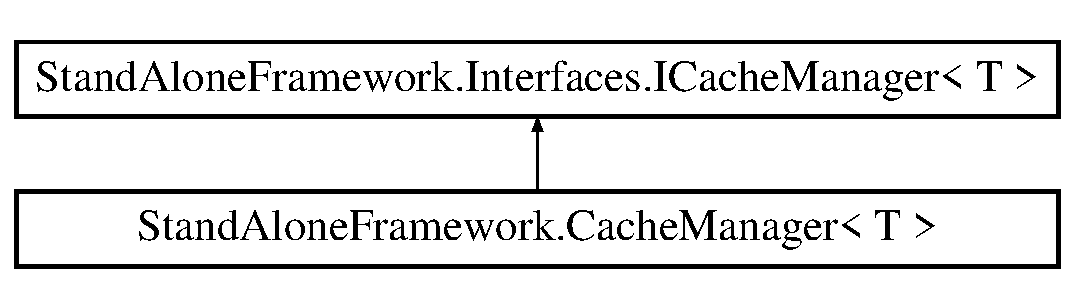
\includegraphics[height=2.000000cm]{class_stand_alone_framework_1_1_cache_manager_3_01_t_01_4}
\end{center}
\end{figure}
\subsection*{Public Member Functions}
\begin{DoxyCompactItemize}
\item 
\hyperlink{class_stand_alone_framework_1_1_cache_manager_3_01_t_01_4_a12dfe46d4b252229dc2a039fc5284672}{Cache\+Manager} ()
\begin{DoxyCompactList}\small\item\em Initializes a new instance of the Cache\+Manager\{\+T\} class. \end{DoxyCompactList}\item 
void \hyperlink{class_stand_alone_framework_1_1_cache_manager_3_01_t_01_4_aa50da1a72eee451e267bb4e2927ebb96}{Add\+Object\+To\+Cache} (T instance)
\begin{DoxyCompactList}\small\item\em Adds the object to cache store. \end{DoxyCompactList}\item 
T \hyperlink{class_stand_alone_framework_1_1_cache_manager_3_01_t_01_4_a37a6e63d5523b967266e4abbc778de95}{Get\+Object\+From\+Cache} (int hash\+Code)
\begin{DoxyCompactList}\small\item\em Gets the object from cache store. \end{DoxyCompactList}\item 
void \hyperlink{class_stand_alone_framework_1_1_cache_manager_3_01_t_01_4_a794235bffdaeb6e34a6b715bbeeacdef}{Flush\+Cache} ()
\begin{DoxyCompactList}\small\item\em Flushes the cache store. \end{DoxyCompactList}\end{DoxyCompactItemize}
\subsection*{Protected Types}
\begin{DoxyCompactItemize}
\item 
enum \hyperlink{class_stand_alone_framework_1_1_cache_manager_3_01_t_01_4_ad524db310decad748ac932dfd557e529}{Cache\+Flush\+Reason} \{ \hyperlink{class_stand_alone_framework_1_1_cache_manager_3_01_t_01_4_ad524db310decad748ac932dfd557e529a7a1920d61156abc05a60135aefe8bc67}{Cache\+Flush\+Reason.\+Default}
 \}
\begin{DoxyCompactList}\small\item\em Represents the reasons for flushing the cache \end{DoxyCompactList}\end{DoxyCompactItemize}
\subsection*{Properties}
\begin{DoxyCompactItemize}
\item 
T \hyperlink{class_stand_alone_framework_1_1_cache_manager_3_01_t_01_4_a89d30acfacd8f0272d29c60b87f0be25}{Instance}\hspace{0.3cm}{\ttfamily  \mbox{[}get, set\mbox{]}}
\begin{DoxyCompactList}\small\item\em Gets or sets the instance of the object to either be stored in the cache store or that is retrieved from the cache store. \end{DoxyCompactList}\end{DoxyCompactItemize}


\subsection{Detailed Description}
Acts as a central store for all objects who need to be cached 


\begin{DoxyTemplParams}{Template Parameters}
{\em T} & \\
\hline
\end{DoxyTemplParams}


\subsection{Member Enumeration Documentation}
\hypertarget{class_stand_alone_framework_1_1_cache_manager_3_01_t_01_4_ad524db310decad748ac932dfd557e529}{\index{Stand\+Alone\+Framework\+::\+Cache\+Manager$<$ T $>$@{Stand\+Alone\+Framework\+::\+Cache\+Manager$<$ T $>$}!Cache\+Flush\+Reason@{Cache\+Flush\+Reason}}
\index{Cache\+Flush\+Reason@{Cache\+Flush\+Reason}!Stand\+Alone\+Framework\+::\+Cache\+Manager$<$ T $>$@{Stand\+Alone\+Framework\+::\+Cache\+Manager$<$ T $>$}}
\subsubsection[{Cache\+Flush\+Reason}]{\setlength{\rightskip}{0pt plus 5cm}enum Stand\+Alone\+Framework.\+Cache\+Manager$<$ T $>$.{\bf Cache\+Flush\+Reason}\hspace{0.3cm}{\ttfamily [protected]}}}\label{class_stand_alone_framework_1_1_cache_manager_3_01_t_01_4_ad524db310decad748ac932dfd557e529}


Represents the reasons for flushing the cache 

\begin{Desc}
\item[Enumerator]\par
\begin{description}
\index{Default@{Default}!Stand\+Alone\+Framework\+::\+Cache\+Manager$<$ T $>$@{Stand\+Alone\+Framework\+::\+Cache\+Manager$<$ T $>$}}\index{Stand\+Alone\+Framework\+::\+Cache\+Manager$<$ T $>$@{Stand\+Alone\+Framework\+::\+Cache\+Manager$<$ T $>$}!Default@{Default}}\item[{\em 
\hypertarget{class_stand_alone_framework_1_1_cache_manager_3_01_t_01_4_ad524db310decad748ac932dfd557e529a7a1920d61156abc05a60135aefe8bc67}{Default}\label{class_stand_alone_framework_1_1_cache_manager_3_01_t_01_4_ad524db310decad748ac932dfd557e529a7a1920d61156abc05a60135aefe8bc67}
}]Represents the default reason for the cache being flushed. Will expand on this soon \end{description}
\end{Desc}


\subsection{Constructor \& Destructor Documentation}
\hypertarget{class_stand_alone_framework_1_1_cache_manager_3_01_t_01_4_a12dfe46d4b252229dc2a039fc5284672}{\index{Stand\+Alone\+Framework\+::\+Cache\+Manager$<$ T $>$@{Stand\+Alone\+Framework\+::\+Cache\+Manager$<$ T $>$}!Cache\+Manager@{Cache\+Manager}}
\index{Cache\+Manager@{Cache\+Manager}!Stand\+Alone\+Framework\+::\+Cache\+Manager$<$ T $>$@{Stand\+Alone\+Framework\+::\+Cache\+Manager$<$ T $>$}}
\subsubsection[{Cache\+Manager}]{\setlength{\rightskip}{0pt plus 5cm}Stand\+Alone\+Framework.\+Cache\+Manager$<$ T $>$.Cache\+Manager (
\begin{DoxyParamCaption}
{}
\end{DoxyParamCaption}
)}}\label{class_stand_alone_framework_1_1_cache_manager_3_01_t_01_4_a12dfe46d4b252229dc2a039fc5284672}


Initializes a new instance of the Cache\+Manager\{\+T\} class. 



\subsection{Member Function Documentation}
\hypertarget{class_stand_alone_framework_1_1_cache_manager_3_01_t_01_4_aa50da1a72eee451e267bb4e2927ebb96}{\index{Stand\+Alone\+Framework\+::\+Cache\+Manager$<$ T $>$@{Stand\+Alone\+Framework\+::\+Cache\+Manager$<$ T $>$}!Add\+Object\+To\+Cache@{Add\+Object\+To\+Cache}}
\index{Add\+Object\+To\+Cache@{Add\+Object\+To\+Cache}!Stand\+Alone\+Framework\+::\+Cache\+Manager$<$ T $>$@{Stand\+Alone\+Framework\+::\+Cache\+Manager$<$ T $>$}}
\subsubsection[{Add\+Object\+To\+Cache}]{\setlength{\rightskip}{0pt plus 5cm}void Stand\+Alone\+Framework.\+Cache\+Manager$<$ T $>$.Add\+Object\+To\+Cache (
\begin{DoxyParamCaption}
\item[{T}]{instance}
\end{DoxyParamCaption}
)}}\label{class_stand_alone_framework_1_1_cache_manager_3_01_t_01_4_aa50da1a72eee451e267bb4e2927ebb96}


Adds the object to cache store. 


\begin{DoxyParams}{Parameters}
{\em instance} & The instance.\\
\hline
\end{DoxyParams}


Implements \hyperlink{interface_stand_alone_framework_1_1_interfaces_1_1_i_cache_manager_3_01_t_01_4_ad0c1608fcc47c31a0afa49f41d516cb4}{Stand\+Alone\+Framework.\+Interfaces.\+I\+Cache\+Manager$<$ T $>$}.

\hypertarget{class_stand_alone_framework_1_1_cache_manager_3_01_t_01_4_a794235bffdaeb6e34a6b715bbeeacdef}{\index{Stand\+Alone\+Framework\+::\+Cache\+Manager$<$ T $>$@{Stand\+Alone\+Framework\+::\+Cache\+Manager$<$ T $>$}!Flush\+Cache@{Flush\+Cache}}
\index{Flush\+Cache@{Flush\+Cache}!Stand\+Alone\+Framework\+::\+Cache\+Manager$<$ T $>$@{Stand\+Alone\+Framework\+::\+Cache\+Manager$<$ T $>$}}
\subsubsection[{Flush\+Cache}]{\setlength{\rightskip}{0pt plus 5cm}void Stand\+Alone\+Framework.\+Cache\+Manager$<$ T $>$.Flush\+Cache (
\begin{DoxyParamCaption}
{}
\end{DoxyParamCaption}
)}}\label{class_stand_alone_framework_1_1_cache_manager_3_01_t_01_4_a794235bffdaeb6e34a6b715bbeeacdef}


Flushes the cache store. 



Implements \hyperlink{interface_stand_alone_framework_1_1_interfaces_1_1_i_cache_manager_3_01_t_01_4_aaedd6cf3b69897bac84bf4ddbad1fdb4}{Stand\+Alone\+Framework.\+Interfaces.\+I\+Cache\+Manager$<$ T $>$}.

\hypertarget{class_stand_alone_framework_1_1_cache_manager_3_01_t_01_4_a37a6e63d5523b967266e4abbc778de95}{\index{Stand\+Alone\+Framework\+::\+Cache\+Manager$<$ T $>$@{Stand\+Alone\+Framework\+::\+Cache\+Manager$<$ T $>$}!Get\+Object\+From\+Cache@{Get\+Object\+From\+Cache}}
\index{Get\+Object\+From\+Cache@{Get\+Object\+From\+Cache}!Stand\+Alone\+Framework\+::\+Cache\+Manager$<$ T $>$@{Stand\+Alone\+Framework\+::\+Cache\+Manager$<$ T $>$}}
\subsubsection[{Get\+Object\+From\+Cache}]{\setlength{\rightskip}{0pt plus 5cm}T Stand\+Alone\+Framework.\+Cache\+Manager$<$ T $>$.Get\+Object\+From\+Cache (
\begin{DoxyParamCaption}
\item[{int}]{hash\+Code}
\end{DoxyParamCaption}
)}}\label{class_stand_alone_framework_1_1_cache_manager_3_01_t_01_4_a37a6e63d5523b967266e4abbc778de95}


Gets the object from cache store. 


\begin{DoxyParams}{Parameters}
{\em hash\+Code} & The hash code.\\
\hline
\end{DoxyParams}
\begin{DoxyReturn}{Returns}
T.
\end{DoxyReturn}


Implements \hyperlink{interface_stand_alone_framework_1_1_interfaces_1_1_i_cache_manager_3_01_t_01_4_ab9c4fc7d4950da75c9bddd22634bd1f3}{Stand\+Alone\+Framework.\+Interfaces.\+I\+Cache\+Manager$<$ T $>$}.



\subsection{Property Documentation}
\hypertarget{class_stand_alone_framework_1_1_cache_manager_3_01_t_01_4_a89d30acfacd8f0272d29c60b87f0be25}{\index{Stand\+Alone\+Framework\+::\+Cache\+Manager$<$ T $>$@{Stand\+Alone\+Framework\+::\+Cache\+Manager$<$ T $>$}!Instance@{Instance}}
\index{Instance@{Instance}!Stand\+Alone\+Framework\+::\+Cache\+Manager$<$ T $>$@{Stand\+Alone\+Framework\+::\+Cache\+Manager$<$ T $>$}}
\subsubsection[{Instance}]{\setlength{\rightskip}{0pt plus 5cm}T Stand\+Alone\+Framework.\+Cache\+Manager$<$ T $>$.Instance\hspace{0.3cm}{\ttfamily [get]}, {\ttfamily [set]}, {\ttfamily [protected]}}}\label{class_stand_alone_framework_1_1_cache_manager_3_01_t_01_4_a89d30acfacd8f0272d29c60b87f0be25}


Gets or sets the instance of the object to either be stored in the cache store or that is retrieved from the cache store. 

The instance.

The documentation for this class was generated from the following file\+:\begin{DoxyCompactItemize}
\item 
C\+:/\+Users/\+Charles Trent Spare/\+Documents/\+Source Control/\+Repositories/\+Development\+Projects/\+Stand\+Alone\+Framework/\+Stand\+Alone\+Framework/\+Cache\+Manager/\hyperlink{_cache_manager_8cs}{Cache\+Manager.\+cs}\end{DoxyCompactItemize}

\hypertarget{class_stand_alone_framework_test_1_1_stateful_tests_1_1_cache_manager_1_1_cache_manger_test_fixture}{\section{Stand\+Alone\+Framework\+Test.\+Stateful\+Tests.\+Cache\+Manager.\+Cache\+Manger\+Test\+Fixture Class Reference}
\label{class_stand_alone_framework_test_1_1_stateful_tests_1_1_cache_manager_1_1_cache_manger_test_fixture}\index{Stand\+Alone\+Framework\+Test.\+Stateful\+Tests.\+Cache\+Manager.\+Cache\+Manger\+Test\+Fixture@{Stand\+Alone\+Framework\+Test.\+Stateful\+Tests.\+Cache\+Manager.\+Cache\+Manger\+Test\+Fixture}}
}
\subsection*{Public Member Functions}
\begin{DoxyCompactItemize}
\item 
void \hyperlink{class_stand_alone_framework_test_1_1_stateful_tests_1_1_cache_manager_1_1_cache_manger_test_fixture_a25291a408d96941a7bbe1d58abb3b562}{Can\+Get\+Object\+From\+Cache} ()
\end{DoxyCompactItemize}


\subsection{Member Function Documentation}
\hypertarget{class_stand_alone_framework_test_1_1_stateful_tests_1_1_cache_manager_1_1_cache_manger_test_fixture_a25291a408d96941a7bbe1d58abb3b562}{\index{Stand\+Alone\+Framework\+Test\+::\+Stateful\+Tests\+::\+Cache\+Manager\+::\+Cache\+Manger\+Test\+Fixture@{Stand\+Alone\+Framework\+Test\+::\+Stateful\+Tests\+::\+Cache\+Manager\+::\+Cache\+Manger\+Test\+Fixture}!Can\+Get\+Object\+From\+Cache@{Can\+Get\+Object\+From\+Cache}}
\index{Can\+Get\+Object\+From\+Cache@{Can\+Get\+Object\+From\+Cache}!Stand\+Alone\+Framework\+Test\+::\+Stateful\+Tests\+::\+Cache\+Manager\+::\+Cache\+Manger\+Test\+Fixture@{Stand\+Alone\+Framework\+Test\+::\+Stateful\+Tests\+::\+Cache\+Manager\+::\+Cache\+Manger\+Test\+Fixture}}
\subsubsection[{Can\+Get\+Object\+From\+Cache}]{\setlength{\rightskip}{0pt plus 5cm}void Stand\+Alone\+Framework\+Test.\+Stateful\+Tests.\+Cache\+Manager.\+Cache\+Manger\+Test\+Fixture.\+Can\+Get\+Object\+From\+Cache (
\begin{DoxyParamCaption}
{}
\end{DoxyParamCaption}
)}}\label{class_stand_alone_framework_test_1_1_stateful_tests_1_1_cache_manager_1_1_cache_manger_test_fixture_a25291a408d96941a7bbe1d58abb3b562}


The documentation for this class was generated from the following file\+:\begin{DoxyCompactItemize}
\item 
C\+:/\+Users/\+Charles Trent Spare/\+Documents/\+Source Control/\+Repositories/\+Development\+Projects/\+Stand\+Alone\+Framework/\+Stand\+Alone\+Framework/\+Stand\+Alone\+Framework\+Test/\+Stateful\+Tests/\+Cache\+Manager/\hyperlink{_cache_manger_test_fixture_8cs}{Cache\+Manger\+Test\+Fixture.\+cs}\end{DoxyCompactItemize}

\hypertarget{class_stand_alone_framework_1_1_code_contract_validator}{\section{Stand\+Alone\+Framework.\+Code\+Contract\+Validator Class Reference}
\label{class_stand_alone_framework_1_1_code_contract_validator}\index{Stand\+Alone\+Framework.\+Code\+Contract\+Validator@{Stand\+Alone\+Framework.\+Code\+Contract\+Validator}}
}


Acts as a code contract validator. This is needed to ensure that all contracts conditions are met prior to any code execution  


\subsection*{Static Public Member Functions}
\begin{DoxyCompactItemize}
\item 
static void \hyperlink{class_stand_alone_framework_1_1_code_contract_validator_aa47caa22c758b103e35f5e305738d5a2}{Argument\+Cannot\+Be\+Null} (object argument, string object\+Friendly\+Name)
\begin{DoxyCompactList}\small\item\em Validates if critical arguments are cannot be null. \end{DoxyCompactList}\item 
static void \hyperlink{class_stand_alone_framework_1_1_code_contract_validator_a448af5fcb383e17a3099d658d9b3fa0e}{Method\+Signature\+Type\+Match} (\hyperlink{namespace_stand_alone_framework_1_1_factories_1_1_method_factory_a03ffbf0d8e733b86d0ac29ae38dd4241}{Method\+Return\+Type} method\+Return\+Type, \hyperlink{namespace_stand_alone_framework_1_1_factories_1_1_method_factory_aeb6e05dc016e73b072faae5a5d275f6a}{Method\+Type} method\+Type)
\begin{DoxyCompactList}\small\item\em Validates if the method's return type matches the signature \end{DoxyCompactList}\end{DoxyCompactItemize}


\subsection{Detailed Description}
Acts as a code contract validator. This is needed to ensure that all contracts conditions are met prior to any code execution 



\subsection{Member Function Documentation}
\hypertarget{class_stand_alone_framework_1_1_code_contract_validator_aa47caa22c758b103e35f5e305738d5a2}{\index{Stand\+Alone\+Framework\+::\+Code\+Contract\+Validator@{Stand\+Alone\+Framework\+::\+Code\+Contract\+Validator}!Argument\+Cannot\+Be\+Null@{Argument\+Cannot\+Be\+Null}}
\index{Argument\+Cannot\+Be\+Null@{Argument\+Cannot\+Be\+Null}!Stand\+Alone\+Framework\+::\+Code\+Contract\+Validator@{Stand\+Alone\+Framework\+::\+Code\+Contract\+Validator}}
\subsubsection[{Argument\+Cannot\+Be\+Null}]{\setlength{\rightskip}{0pt plus 5cm}static void Stand\+Alone\+Framework.\+Code\+Contract\+Validator.\+Argument\+Cannot\+Be\+Null (
\begin{DoxyParamCaption}
\item[{object}]{argument, }
\item[{string}]{object\+Friendly\+Name}
\end{DoxyParamCaption}
)\hspace{0.3cm}{\ttfamily [static]}}}\label{class_stand_alone_framework_1_1_code_contract_validator_aa47caa22c758b103e35f5e305738d5a2}


Validates if critical arguments are cannot be null. 


\begin{DoxyParams}{Parameters}
{\em argument} & The argument.\\
\hline
{\em object\+Friendly\+Name} & Name of the object friendly.\\
\hline
\end{DoxyParams}

\begin{DoxyExceptions}{Exceptions}
{\em System.\+Exception} & \\
\hline
\end{DoxyExceptions}
\hypertarget{class_stand_alone_framework_1_1_code_contract_validator_a448af5fcb383e17a3099d658d9b3fa0e}{\index{Stand\+Alone\+Framework\+::\+Code\+Contract\+Validator@{Stand\+Alone\+Framework\+::\+Code\+Contract\+Validator}!Method\+Signature\+Type\+Match@{Method\+Signature\+Type\+Match}}
\index{Method\+Signature\+Type\+Match@{Method\+Signature\+Type\+Match}!Stand\+Alone\+Framework\+::\+Code\+Contract\+Validator@{Stand\+Alone\+Framework\+::\+Code\+Contract\+Validator}}
\subsubsection[{Method\+Signature\+Type\+Match}]{\setlength{\rightskip}{0pt plus 5cm}static void Stand\+Alone\+Framework.\+Code\+Contract\+Validator.\+Method\+Signature\+Type\+Match (
\begin{DoxyParamCaption}
\item[{{\bf Method\+Return\+Type}}]{method\+Return\+Type, }
\item[{{\bf Method\+Type}}]{method\+Type}
\end{DoxyParamCaption}
)\hspace{0.3cm}{\ttfamily [static]}}}\label{class_stand_alone_framework_1_1_code_contract_validator_a448af5fcb383e17a3099d658d9b3fa0e}


Validates if the method's return type matches the signature 


\begin{DoxyParams}{Parameters}
{\em method\+Return\+Type} & Return type of the method return.\\
\hline
{\em method\+Type} & Type of the method.\\
\hline
\end{DoxyParams}

\begin{DoxyExceptions}{Exceptions}
{\em System.\+Exception} & \\
\hline
\end{DoxyExceptions}


The documentation for this class was generated from the following file\+:\begin{DoxyCompactItemize}
\item 
C\+:/\+Users/\+Charles Trent Spare/\+Documents/\+Source Control/\+Repositories/\+Development\+Projects/\+Stand\+Alone\+Framework/\+Stand\+Alone\+Framework/\+Code\+Contract\+Validator/\hyperlink{_code_contract_validator_8cs}{Code\+Contract\+Validator.\+cs}\end{DoxyCompactItemize}

\hypertarget{class_stand_alone_framework_1_1_data_wrapper}{\section{Stand\+Alone\+Framework.\+Data\+Wrapper Class Reference}
\label{class_stand_alone_framework_1_1_data_wrapper}\index{Stand\+Alone\+Framework.\+Data\+Wrapper@{Stand\+Alone\+Framework.\+Data\+Wrapper}}
}


Acts as a wrapper for the arguments that need to be passed into the method  


\subsection*{Public Attributes}
\begin{DoxyCompactItemize}
\item 
int \hyperlink{class_stand_alone_framework_1_1_data_wrapper_a35e406cf3d38047236b60b94618e2181}{x\+Value}
\begin{DoxyCompactList}\small\item\em Dummy Value \end{DoxyCompactList}\end{DoxyCompactItemize}
\subsection*{Properties}
\begin{DoxyCompactItemize}
\item 
string \hyperlink{class_stand_alone_framework_1_1_data_wrapper_a37c856045eb222ea573dee4a2e64e34d}{Argument}\hspace{0.3cm}{\ttfamily  \mbox{[}get, set\mbox{]}}
\begin{DoxyCompactList}\small\item\em This could represent a dummy value \end{DoxyCompactList}\end{DoxyCompactItemize}


\subsection{Detailed Description}
Acts as a wrapper for the arguments that need to be passed into the method 



\subsection{Member Data Documentation}
\hypertarget{class_stand_alone_framework_1_1_data_wrapper_a35e406cf3d38047236b60b94618e2181}{\index{Stand\+Alone\+Framework\+::\+Data\+Wrapper@{Stand\+Alone\+Framework\+::\+Data\+Wrapper}!x\+Value@{x\+Value}}
\index{x\+Value@{x\+Value}!Stand\+Alone\+Framework\+::\+Data\+Wrapper@{Stand\+Alone\+Framework\+::\+Data\+Wrapper}}
\subsubsection[{x\+Value}]{\setlength{\rightskip}{0pt plus 5cm}int Stand\+Alone\+Framework.\+Data\+Wrapper.\+x\+Value}}\label{class_stand_alone_framework_1_1_data_wrapper_a35e406cf3d38047236b60b94618e2181}


Dummy Value 



\subsection{Property Documentation}
\hypertarget{class_stand_alone_framework_1_1_data_wrapper_a37c856045eb222ea573dee4a2e64e34d}{\index{Stand\+Alone\+Framework\+::\+Data\+Wrapper@{Stand\+Alone\+Framework\+::\+Data\+Wrapper}!Argument@{Argument}}
\index{Argument@{Argument}!Stand\+Alone\+Framework\+::\+Data\+Wrapper@{Stand\+Alone\+Framework\+::\+Data\+Wrapper}}
\subsubsection[{Argument}]{\setlength{\rightskip}{0pt plus 5cm}string Stand\+Alone\+Framework.\+Data\+Wrapper.\+Argument\hspace{0.3cm}{\ttfamily [get]}, {\ttfamily [set]}}}\label{class_stand_alone_framework_1_1_data_wrapper_a37c856045eb222ea573dee4a2e64e34d}


This could represent a dummy value 

The argument.

The documentation for this class was generated from the following file\+:\begin{DoxyCompactItemize}
\item 
C\+:/\+Users/\+Charles Trent Spare/\+Documents/\+Source Control/\+Repositories/\+Development\+Projects/\+Stand\+Alone\+Framework/\+Stand\+Alone\+Framework/\hyperlink{_data_wrapper_8cs}{Data\+Wrapper.\+cs}\end{DoxyCompactItemize}

\hypertarget{class_stand_alone_framework_1_1_dyamic_invoker}{\section{Stand\+Alone\+Framework.\+Dyamic\+Invoker Class Reference}
\label{class_stand_alone_framework_1_1_dyamic_invoker}\index{Stand\+Alone\+Framework.\+Dyamic\+Invoker@{Stand\+Alone\+Framework.\+Dyamic\+Invoker}}
}


Represents a class that is able to execute a method without knowing the internal workings. It also wraps the method call in an error handler and defers all error handling the the {\ttfamily \hyperlink{class_stand_alone_framework_1_1_error_manager}{Error\+Manager} class}  


Inheritance diagram for Stand\+Alone\+Framework.\+Dyamic\+Invoker\+:\begin{figure}[H]
\begin{center}
\leavevmode
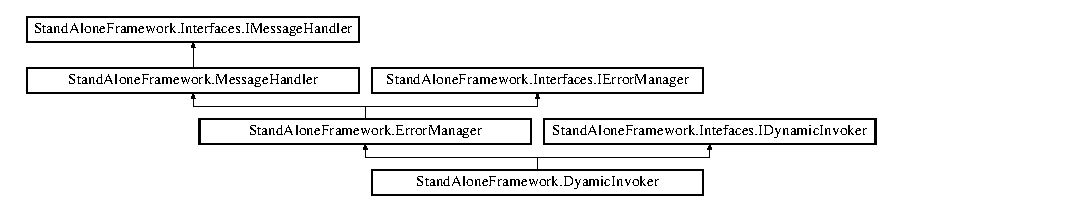
\includegraphics[height=2.400857cm]{class_stand_alone_framework_1_1_dyamic_invoker}
\end{center}
\end{figure}
\subsection*{Public Member Functions}
\begin{DoxyCompactItemize}
\item 
\hyperlink{class_stand_alone_framework_1_1_framework_classes_1_1_invocation_result}{Invocation\+Result} \hyperlink{class_stand_alone_framework_1_1_dyamic_invoker_afa62776cb39ce4e31221dc1373440d06}{Invoke\+Method} (\hyperlink{class_stand_alone_framework_1_1_factories_1_1_method_factory_1_1_method_wrapper}{Method\+Wrapper} method\+Wrapper)
\begin{DoxyCompactList}\small\item\em Invokes the method. \end{DoxyCompactList}\end{DoxyCompactItemize}
\subsection*{Additional Inherited Members}


\subsection{Detailed Description}
Represents a class that is able to execute a method without knowing the internal workings. It also wraps the method call in an error handler and defers all error handling the the {\ttfamily \hyperlink{class_stand_alone_framework_1_1_error_manager}{Error\+Manager} class} 



\subsection{Member Function Documentation}
\hypertarget{class_stand_alone_framework_1_1_dyamic_invoker_afa62776cb39ce4e31221dc1373440d06}{\index{Stand\+Alone\+Framework\+::\+Dyamic\+Invoker@{Stand\+Alone\+Framework\+::\+Dyamic\+Invoker}!Invoke\+Method@{Invoke\+Method}}
\index{Invoke\+Method@{Invoke\+Method}!Stand\+Alone\+Framework\+::\+Dyamic\+Invoker@{Stand\+Alone\+Framework\+::\+Dyamic\+Invoker}}
\subsubsection[{Invoke\+Method}]{\setlength{\rightskip}{0pt plus 5cm}{\bf Invocation\+Result} Stand\+Alone\+Framework.\+Dyamic\+Invoker.\+Invoke\+Method (
\begin{DoxyParamCaption}
\item[{{\bf Method\+Wrapper}}]{method\+Wrapper}
\end{DoxyParamCaption}
)}}\label{class_stand_alone_framework_1_1_dyamic_invoker_afa62776cb39ce4e31221dc1373440d06}


Invokes the method. 


\begin{DoxyParams}{Parameters}
{\em method\+Wrapper} & The method wrapper.\\
\hline
\end{DoxyParams}
\begin{DoxyReturn}{Returns}
Invocation\+Result.
\end{DoxyReturn}


Implements \hyperlink{interface_stand_alone_framework_1_1_intefaces_1_1_i_dynamic_invoker_ad3978a717b76fbd44c1f8ce6c08564cc}{Stand\+Alone\+Framework.\+Intefaces.\+I\+Dynamic\+Invoker}.



The documentation for this class was generated from the following file\+:\begin{DoxyCompactItemize}
\item 
C\+:/\+Users/\+Charles Trent Spare/\+Documents/\+Source Control/\+Repositories/\+Development\+Projects/\+Stand\+Alone\+Framework/\+Stand\+Alone\+Framework/\+Dynamic\+Invoker/\hyperlink{_dyamic_invoker_8cs}{Dyamic\+Invoker.\+cs}\end{DoxyCompactItemize}

\hypertarget{class_stand_alone_framework_1_1_error_manager}{\section{Stand\+Alone\+Framework.\+Error\+Manager Class Reference}
\label{class_stand_alone_framework_1_1_error_manager}\index{Stand\+Alone\+Framework.\+Error\+Manager@{Stand\+Alone\+Framework.\+Error\+Manager}}
}


Acts as the central error handling component during method execution.  


Inheritance diagram for Stand\+Alone\+Framework.\+Error\+Manager\+:\begin{figure}[H]
\begin{center}
\leavevmode
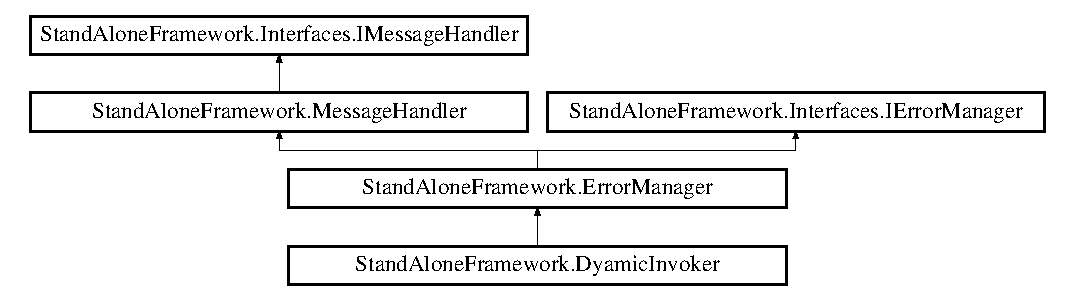
\includegraphics[height=3.601286cm]{class_stand_alone_framework_1_1_error_manager}
\end{center}
\end{figure}
\subsection*{Public Member Functions}
\begin{DoxyCompactItemize}
\item 
void \hyperlink{class_stand_alone_framework_1_1_error_manager_a0f6fe7860c545b64f9adaeae7a7b5919}{Handle\+Error\+Messages} (Exception exception, ref \hyperlink{class_stand_alone_framework_1_1_framework_classes_1_1_invocation_result}{Invocation\+Result} \hyperlink{class_stand_alone_framework_1_1_error_manager_a25023f8540577f3d5d901f2569c3f2ec}{invocation\+Result})
\begin{DoxyCompactList}\small\item\em Handles the error messages that are encountered during the method execution. \end{DoxyCompactList}\end{DoxyCompactItemize}
\subsection*{Protected Attributes}
\begin{DoxyCompactItemize}
\item 
\hyperlink{class_stand_alone_framework_1_1_framework_classes_1_1_invocation_result}{Invocation\+Result} \hyperlink{class_stand_alone_framework_1_1_error_manager_a25023f8540577f3d5d901f2569c3f2ec}{invocation\+Result}
\begin{DoxyCompactList}\small\item\em The invocation result that is returned by reference after the method execution \end{DoxyCompactList}\end{DoxyCompactItemize}
\subsection*{Properties}
\begin{DoxyCompactItemize}
\item 
\hyperlink{class_stand_alone_framework_1_1_framework_classes_1_1_invocation_result}{Invocation\+Result} \hyperlink{class_stand_alone_framework_1_1_error_manager_a98353b3c901cdfb95f1c8dc3499ebb13}{Invocation\+Result}\hspace{0.3cm}{\ttfamily  \mbox{[}get, set\mbox{]}}
\begin{DoxyCompactList}\small\item\em Gets or sets the invocation result that is returned to the callee after method execution. \end{DoxyCompactList}\end{DoxyCompactItemize}


\subsection{Detailed Description}
Acts as the central error handling component during method execution. 



\subsection{Member Function Documentation}
\hypertarget{class_stand_alone_framework_1_1_error_manager_a0f6fe7860c545b64f9adaeae7a7b5919}{\index{Stand\+Alone\+Framework\+::\+Error\+Manager@{Stand\+Alone\+Framework\+::\+Error\+Manager}!Handle\+Error\+Messages@{Handle\+Error\+Messages}}
\index{Handle\+Error\+Messages@{Handle\+Error\+Messages}!Stand\+Alone\+Framework\+::\+Error\+Manager@{Stand\+Alone\+Framework\+::\+Error\+Manager}}
\subsubsection[{Handle\+Error\+Messages}]{\setlength{\rightskip}{0pt plus 5cm}void Stand\+Alone\+Framework.\+Error\+Manager.\+Handle\+Error\+Messages (
\begin{DoxyParamCaption}
\item[{Exception}]{exception, }
\item[{ref {\bf Invocation\+Result}}]{invocation\+Result}
\end{DoxyParamCaption}
)}}\label{class_stand_alone_framework_1_1_error_manager_a0f6fe7860c545b64f9adaeae7a7b5919}


Handles the error messages that are encountered during the method execution. 


\begin{DoxyParams}{Parameters}
{\em exception} & The exception.\\
\hline
{\em invocation\+Result} & The invocation result.\\
\hline
\end{DoxyParams}


Implements \hyperlink{interface_stand_alone_framework_1_1_interfaces_1_1_i_error_manager_a54b9927bcf2778d3626a60f7439e41eb}{Stand\+Alone\+Framework.\+Interfaces.\+I\+Error\+Manager}.



\subsection{Member Data Documentation}
\hypertarget{class_stand_alone_framework_1_1_error_manager_a25023f8540577f3d5d901f2569c3f2ec}{\index{Stand\+Alone\+Framework\+::\+Error\+Manager@{Stand\+Alone\+Framework\+::\+Error\+Manager}!invocation\+Result@{invocation\+Result}}
\index{invocation\+Result@{invocation\+Result}!Stand\+Alone\+Framework\+::\+Error\+Manager@{Stand\+Alone\+Framework\+::\+Error\+Manager}}
\subsubsection[{invocation\+Result}]{\setlength{\rightskip}{0pt plus 5cm}{\bf Invocation\+Result} Stand\+Alone\+Framework.\+Error\+Manager.\+invocation\+Result\hspace{0.3cm}{\ttfamily [protected]}}}\label{class_stand_alone_framework_1_1_error_manager_a25023f8540577f3d5d901f2569c3f2ec}


The invocation result that is returned by reference after the method execution 



\subsection{Property Documentation}
\hypertarget{class_stand_alone_framework_1_1_error_manager_a98353b3c901cdfb95f1c8dc3499ebb13}{\index{Stand\+Alone\+Framework\+::\+Error\+Manager@{Stand\+Alone\+Framework\+::\+Error\+Manager}!Invocation\+Result@{Invocation\+Result}}
\index{Invocation\+Result@{Invocation\+Result}!Stand\+Alone\+Framework\+::\+Error\+Manager@{Stand\+Alone\+Framework\+::\+Error\+Manager}}
\subsubsection[{Invocation\+Result}]{\setlength{\rightskip}{0pt plus 5cm}{\bf Invocation\+Result} Stand\+Alone\+Framework.\+Error\+Manager.\+Invocation\+Result\hspace{0.3cm}{\ttfamily [get]}, {\ttfamily [set]}, {\ttfamily [protected]}}}\label{class_stand_alone_framework_1_1_error_manager_a98353b3c901cdfb95f1c8dc3499ebb13}


Gets or sets the invocation result that is returned to the callee after method execution. 

The invocation result.

The documentation for this class was generated from the following file\+:\begin{DoxyCompactItemize}
\item 
C\+:/\+Users/\+Charles Trent Spare/\+Documents/\+Source Control/\+Repositories/\+Development\+Projects/\+Stand\+Alone\+Framework/\+Stand\+Alone\+Framework/\+Error\+Manager/\hyperlink{_error_manager_8cs}{Error\+Manager.\+cs}\end{DoxyCompactItemize}

\hypertarget{interface_stand_alone_framework_1_1_interfaces_1_1_i_cache_manager_3_01_t_01_4}{\section{Stand\+Alone\+Framework.\+Interfaces.\+I\+Cache\+Manager$<$ T $>$ Interface Template Reference}
\label{interface_stand_alone_framework_1_1_interfaces_1_1_i_cache_manager_3_01_t_01_4}\index{Stand\+Alone\+Framework.\+Interfaces.\+I\+Cache\+Manager$<$ T $>$@{Stand\+Alone\+Framework.\+Interfaces.\+I\+Cache\+Manager$<$ T $>$}}
}


The Cache\+Manager's contract  


Inheritance diagram for Stand\+Alone\+Framework.\+Interfaces.\+I\+Cache\+Manager$<$ T $>$\+:\begin{figure}[H]
\begin{center}
\leavevmode
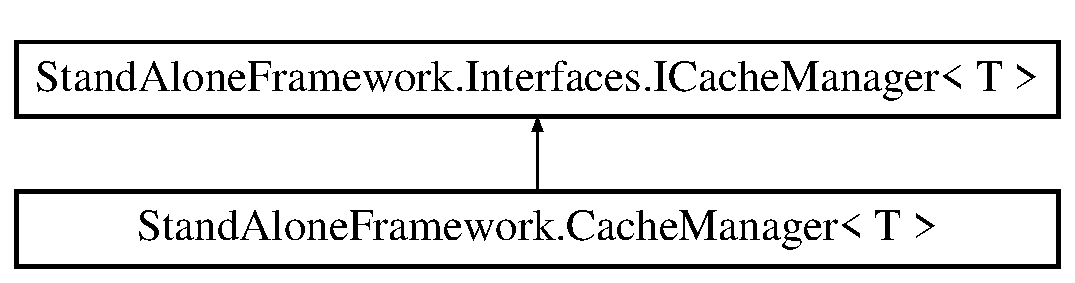
\includegraphics[height=2.000000cm]{interface_stand_alone_framework_1_1_interfaces_1_1_i_cache_manager_3_01_t_01_4}
\end{center}
\end{figure}
\subsection*{Public Member Functions}
\begin{DoxyCompactItemize}
\item 
void \hyperlink{interface_stand_alone_framework_1_1_interfaces_1_1_i_cache_manager_3_01_t_01_4_ad0c1608fcc47c31a0afa49f41d516cb4}{Add\+Object\+To\+Cache} (T instance)
\begin{DoxyCompactList}\small\item\em Adds the object to cache store. \end{DoxyCompactList}\item 
T \hyperlink{interface_stand_alone_framework_1_1_interfaces_1_1_i_cache_manager_3_01_t_01_4_ab9c4fc7d4950da75c9bddd22634bd1f3}{Get\+Object\+From\+Cache} (int hash\+Code)
\begin{DoxyCompactList}\small\item\em Gets the object from cache store. \end{DoxyCompactList}\item 
void \hyperlink{interface_stand_alone_framework_1_1_interfaces_1_1_i_cache_manager_3_01_t_01_4_aaedd6cf3b69897bac84bf4ddbad1fdb4}{Flush\+Cache} ()
\begin{DoxyCompactList}\small\item\em Flushes the cache store. \end{DoxyCompactList}\end{DoxyCompactItemize}


\subsection{Detailed Description}
The Cache\+Manager's contract 


\begin{DoxyTemplParams}{Template Parameters}
{\em T} & \\
\hline
\end{DoxyTemplParams}


\subsection{Member Function Documentation}
\hypertarget{interface_stand_alone_framework_1_1_interfaces_1_1_i_cache_manager_3_01_t_01_4_ad0c1608fcc47c31a0afa49f41d516cb4}{\index{Stand\+Alone\+Framework\+::\+Interfaces\+::\+I\+Cache\+Manager$<$ T $>$@{Stand\+Alone\+Framework\+::\+Interfaces\+::\+I\+Cache\+Manager$<$ T $>$}!Add\+Object\+To\+Cache@{Add\+Object\+To\+Cache}}
\index{Add\+Object\+To\+Cache@{Add\+Object\+To\+Cache}!Stand\+Alone\+Framework\+::\+Interfaces\+::\+I\+Cache\+Manager$<$ T $>$@{Stand\+Alone\+Framework\+::\+Interfaces\+::\+I\+Cache\+Manager$<$ T $>$}}
\subsubsection[{Add\+Object\+To\+Cache}]{\setlength{\rightskip}{0pt plus 5cm}void Stand\+Alone\+Framework.\+Interfaces.\+I\+Cache\+Manager$<$ T $>$.Add\+Object\+To\+Cache (
\begin{DoxyParamCaption}
\item[{T}]{instance}
\end{DoxyParamCaption}
)}}\label{interface_stand_alone_framework_1_1_interfaces_1_1_i_cache_manager_3_01_t_01_4_ad0c1608fcc47c31a0afa49f41d516cb4}


Adds the object to cache store. 


\begin{DoxyParams}{Parameters}
{\em instance} & The instance.\\
\hline
\end{DoxyParams}


Implemented in \hyperlink{class_stand_alone_framework_1_1_cache_manager_3_01_t_01_4_aa50da1a72eee451e267bb4e2927ebb96}{Stand\+Alone\+Framework.\+Cache\+Manager$<$ T $>$}.

\hypertarget{interface_stand_alone_framework_1_1_interfaces_1_1_i_cache_manager_3_01_t_01_4_aaedd6cf3b69897bac84bf4ddbad1fdb4}{\index{Stand\+Alone\+Framework\+::\+Interfaces\+::\+I\+Cache\+Manager$<$ T $>$@{Stand\+Alone\+Framework\+::\+Interfaces\+::\+I\+Cache\+Manager$<$ T $>$}!Flush\+Cache@{Flush\+Cache}}
\index{Flush\+Cache@{Flush\+Cache}!Stand\+Alone\+Framework\+::\+Interfaces\+::\+I\+Cache\+Manager$<$ T $>$@{Stand\+Alone\+Framework\+::\+Interfaces\+::\+I\+Cache\+Manager$<$ T $>$}}
\subsubsection[{Flush\+Cache}]{\setlength{\rightskip}{0pt plus 5cm}void Stand\+Alone\+Framework.\+Interfaces.\+I\+Cache\+Manager$<$ T $>$.Flush\+Cache (
\begin{DoxyParamCaption}
{}
\end{DoxyParamCaption}
)}}\label{interface_stand_alone_framework_1_1_interfaces_1_1_i_cache_manager_3_01_t_01_4_aaedd6cf3b69897bac84bf4ddbad1fdb4}


Flushes the cache store. 



Implemented in \hyperlink{class_stand_alone_framework_1_1_cache_manager_3_01_t_01_4_a794235bffdaeb6e34a6b715bbeeacdef}{Stand\+Alone\+Framework.\+Cache\+Manager$<$ T $>$}.

\hypertarget{interface_stand_alone_framework_1_1_interfaces_1_1_i_cache_manager_3_01_t_01_4_ab9c4fc7d4950da75c9bddd22634bd1f3}{\index{Stand\+Alone\+Framework\+::\+Interfaces\+::\+I\+Cache\+Manager$<$ T $>$@{Stand\+Alone\+Framework\+::\+Interfaces\+::\+I\+Cache\+Manager$<$ T $>$}!Get\+Object\+From\+Cache@{Get\+Object\+From\+Cache}}
\index{Get\+Object\+From\+Cache@{Get\+Object\+From\+Cache}!Stand\+Alone\+Framework\+::\+Interfaces\+::\+I\+Cache\+Manager$<$ T $>$@{Stand\+Alone\+Framework\+::\+Interfaces\+::\+I\+Cache\+Manager$<$ T $>$}}
\subsubsection[{Get\+Object\+From\+Cache}]{\setlength{\rightskip}{0pt plus 5cm}T Stand\+Alone\+Framework.\+Interfaces.\+I\+Cache\+Manager$<$ T $>$.Get\+Object\+From\+Cache (
\begin{DoxyParamCaption}
\item[{int}]{hash\+Code}
\end{DoxyParamCaption}
)}}\label{interface_stand_alone_framework_1_1_interfaces_1_1_i_cache_manager_3_01_t_01_4_ab9c4fc7d4950da75c9bddd22634bd1f3}


Gets the object from cache store. 


\begin{DoxyParams}{Parameters}
{\em hash\+Code} & The hash code.\\
\hline
\end{DoxyParams}
\begin{DoxyReturn}{Returns}
T.
\end{DoxyReturn}


Implemented in \hyperlink{class_stand_alone_framework_1_1_cache_manager_3_01_t_01_4_a37a6e63d5523b967266e4abbc778de95}{Stand\+Alone\+Framework.\+Cache\+Manager$<$ T $>$}.



The documentation for this interface was generated from the following file\+:\begin{DoxyCompactItemize}
\item 
C\+:/\+Users/\+Charles Trent Spare/\+Documents/\+Source Control/\+Repositories/\+Development\+Projects/\+Stand\+Alone\+Framework/\+Stand\+Alone\+Framework/\+Cache\+Manager/\+Interfaces/\hyperlink{_i_cache_manager_8cs}{I\+Cache\+Manager.\+cs}\end{DoxyCompactItemize}

\hypertarget{interface_stand_alone_framework_1_1_intefaces_1_1_i_dynamic_invoker}{\section{Stand\+Alone\+Framework.\+Intefaces.\+I\+Dynamic\+Invoker Interface Reference}
\label{interface_stand_alone_framework_1_1_intefaces_1_1_i_dynamic_invoker}\index{Stand\+Alone\+Framework.\+Intefaces.\+I\+Dynamic\+Invoker@{Stand\+Alone\+Framework.\+Intefaces.\+I\+Dynamic\+Invoker}}
}


The Dynamic\+Invokers contract  


Inheritance diagram for Stand\+Alone\+Framework.\+Intefaces.\+I\+Dynamic\+Invoker\+:\begin{figure}[H]
\begin{center}
\leavevmode
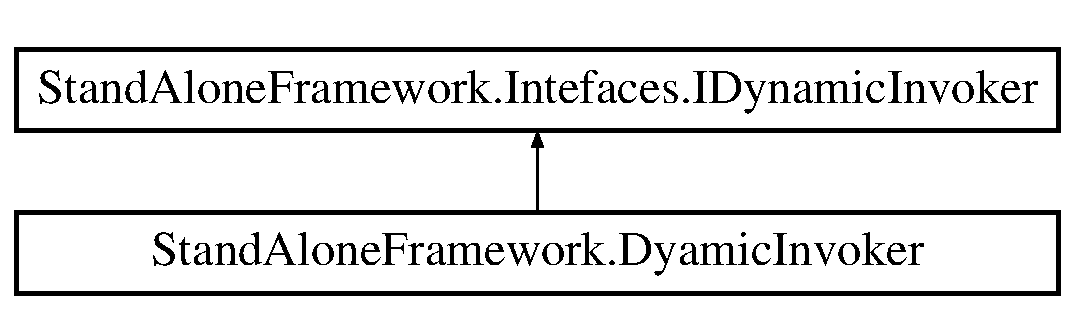
\includegraphics[height=2.000000cm]{interface_stand_alone_framework_1_1_intefaces_1_1_i_dynamic_invoker}
\end{center}
\end{figure}
\subsection*{Public Member Functions}
\begin{DoxyCompactItemize}
\item 
\hyperlink{class_stand_alone_framework_1_1_framework_classes_1_1_invocation_result}{Invocation\+Result} \hyperlink{interface_stand_alone_framework_1_1_intefaces_1_1_i_dynamic_invoker_ad3978a717b76fbd44c1f8ce6c08564cc}{Invoke\+Method} (\hyperlink{class_stand_alone_framework_1_1_factories_1_1_method_factory_1_1_method_wrapper}{Method\+Wrapper} method\+Wrapper)
\begin{DoxyCompactList}\small\item\em Invokes the method. \end{DoxyCompactList}\end{DoxyCompactItemize}


\subsection{Detailed Description}
The Dynamic\+Invokers contract 



\subsection{Member Function Documentation}
\hypertarget{interface_stand_alone_framework_1_1_intefaces_1_1_i_dynamic_invoker_ad3978a717b76fbd44c1f8ce6c08564cc}{\index{Stand\+Alone\+Framework\+::\+Intefaces\+::\+I\+Dynamic\+Invoker@{Stand\+Alone\+Framework\+::\+Intefaces\+::\+I\+Dynamic\+Invoker}!Invoke\+Method@{Invoke\+Method}}
\index{Invoke\+Method@{Invoke\+Method}!Stand\+Alone\+Framework\+::\+Intefaces\+::\+I\+Dynamic\+Invoker@{Stand\+Alone\+Framework\+::\+Intefaces\+::\+I\+Dynamic\+Invoker}}
\subsubsection[{Invoke\+Method}]{\setlength{\rightskip}{0pt plus 5cm}{\bf Invocation\+Result} Stand\+Alone\+Framework.\+Intefaces.\+I\+Dynamic\+Invoker.\+Invoke\+Method (
\begin{DoxyParamCaption}
\item[{{\bf Method\+Wrapper}}]{method\+Wrapper}
\end{DoxyParamCaption}
)}}\label{interface_stand_alone_framework_1_1_intefaces_1_1_i_dynamic_invoker_ad3978a717b76fbd44c1f8ce6c08564cc}


Invokes the method. 


\begin{DoxyParams}{Parameters}
{\em method\+Wrapper} & The method wrapper.\\
\hline
\end{DoxyParams}
\begin{DoxyReturn}{Returns}
Invocation\+Result.
\end{DoxyReturn}


Implemented in \hyperlink{class_stand_alone_framework_1_1_dyamic_invoker_afa62776cb39ce4e31221dc1373440d06}{Stand\+Alone\+Framework.\+Dyamic\+Invoker}.



The documentation for this interface was generated from the following file\+:\begin{DoxyCompactItemize}
\item 
C\+:/\+Users/\+Charles Trent Spare/\+Documents/\+Source Control/\+Repositories/\+Development\+Projects/\+Stand\+Alone\+Framework/\+Stand\+Alone\+Framework/\+Dynamic\+Invoker/\+Intefaces/\hyperlink{_i_dynamic_invoker_8cs}{I\+Dynamic\+Invoker.\+cs}\end{DoxyCompactItemize}

\hypertarget{interface_stand_alone_framework_1_1_interfaces_1_1_i_error_manager}{\section{Stand\+Alone\+Framework.\+Interfaces.\+I\+Error\+Manager Interface Reference}
\label{interface_stand_alone_framework_1_1_interfaces_1_1_i_error_manager}\index{Stand\+Alone\+Framework.\+Interfaces.\+I\+Error\+Manager@{Stand\+Alone\+Framework.\+Interfaces.\+I\+Error\+Manager}}
}


The \hyperlink{class_stand_alone_framework_1_1_error_manager}{Error\+Manager} contract  


Inheritance diagram for Stand\+Alone\+Framework.\+Interfaces.\+I\+Error\+Manager\+:\begin{figure}[H]
\begin{center}
\leavevmode
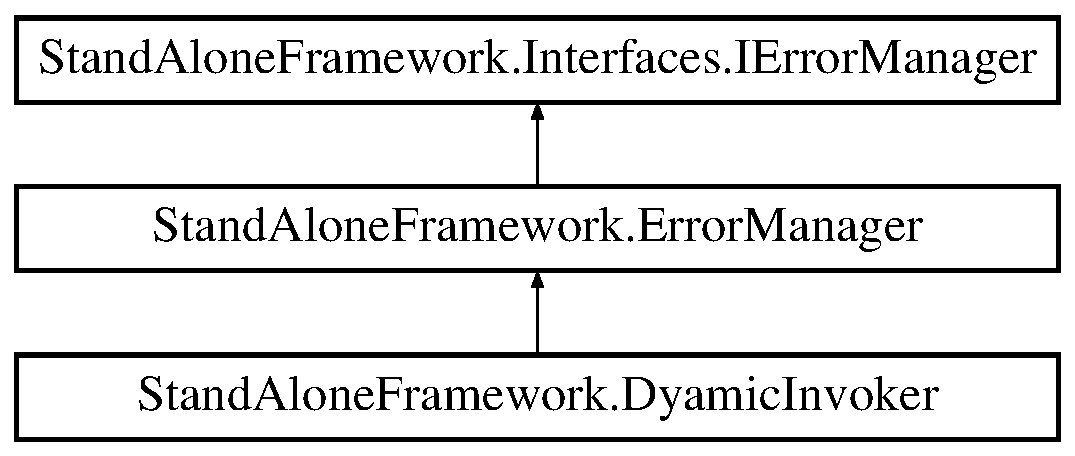
\includegraphics[height=3.000000cm]{interface_stand_alone_framework_1_1_interfaces_1_1_i_error_manager}
\end{center}
\end{figure}
\subsection*{Public Member Functions}
\begin{DoxyCompactItemize}
\item 
void \hyperlink{interface_stand_alone_framework_1_1_interfaces_1_1_i_error_manager_a54b9927bcf2778d3626a60f7439e41eb}{Handle\+Error\+Messages} (Exception exception, ref \hyperlink{class_stand_alone_framework_1_1_framework_classes_1_1_invocation_result}{Invocation\+Result} invocation\+Result)
\begin{DoxyCompactList}\small\item\em Handles the error messages that are encountered during the method execution. \end{DoxyCompactList}\end{DoxyCompactItemize}


\subsection{Detailed Description}
The \hyperlink{class_stand_alone_framework_1_1_error_manager}{Error\+Manager} contract 



\subsection{Member Function Documentation}
\hypertarget{interface_stand_alone_framework_1_1_interfaces_1_1_i_error_manager_a54b9927bcf2778d3626a60f7439e41eb}{\index{Stand\+Alone\+Framework\+::\+Interfaces\+::\+I\+Error\+Manager@{Stand\+Alone\+Framework\+::\+Interfaces\+::\+I\+Error\+Manager}!Handle\+Error\+Messages@{Handle\+Error\+Messages}}
\index{Handle\+Error\+Messages@{Handle\+Error\+Messages}!Stand\+Alone\+Framework\+::\+Interfaces\+::\+I\+Error\+Manager@{Stand\+Alone\+Framework\+::\+Interfaces\+::\+I\+Error\+Manager}}
\subsubsection[{Handle\+Error\+Messages}]{\setlength{\rightskip}{0pt plus 5cm}void Stand\+Alone\+Framework.\+Interfaces.\+I\+Error\+Manager.\+Handle\+Error\+Messages (
\begin{DoxyParamCaption}
\item[{Exception}]{exception, }
\item[{ref {\bf Invocation\+Result}}]{invocation\+Result}
\end{DoxyParamCaption}
)}}\label{interface_stand_alone_framework_1_1_interfaces_1_1_i_error_manager_a54b9927bcf2778d3626a60f7439e41eb}


Handles the error messages that are encountered during the method execution. 


\begin{DoxyParams}{Parameters}
{\em exception} & The exception.\\
\hline
{\em invocation\+Result} & The invocation result.\\
\hline
\end{DoxyParams}


Implemented in \hyperlink{class_stand_alone_framework_1_1_error_manager_a0f6fe7860c545b64f9adaeae7a7b5919}{Stand\+Alone\+Framework.\+Error\+Manager}.



The documentation for this interface was generated from the following file\+:\begin{DoxyCompactItemize}
\item 
C\+:/\+Users/\+Charles Trent Spare/\+Documents/\+Source Control/\+Repositories/\+Development\+Projects/\+Stand\+Alone\+Framework/\+Stand\+Alone\+Framework/\+Error\+Manager/\+Interfaces/\hyperlink{_i_error_manager_8cs}{I\+Error\+Manager.\+cs}\end{DoxyCompactItemize}

\hypertarget{interface_stand_alone_framework_1_1_interfaces_1_1_i_memory_manager}{\section{Stand\+Alone\+Framework.\+Interfaces.\+I\+Memory\+Manager Interface Reference}
\label{interface_stand_alone_framework_1_1_interfaces_1_1_i_memory_manager}\index{Stand\+Alone\+Framework.\+Interfaces.\+I\+Memory\+Manager@{Stand\+Alone\+Framework.\+Interfaces.\+I\+Memory\+Manager}}
}
Inheritance diagram for Stand\+Alone\+Framework.\+Interfaces.\+I\+Memory\+Manager\+:\begin{figure}[H]
\begin{center}
\leavevmode
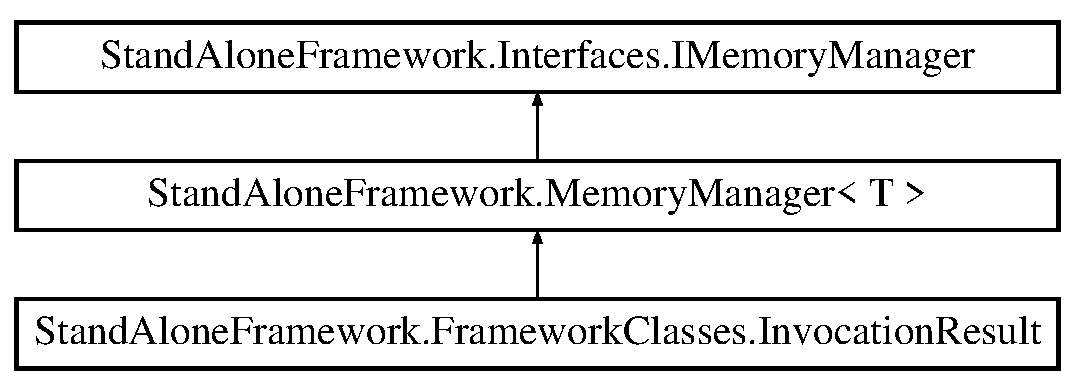
\includegraphics[height=3.000000cm]{interface_stand_alone_framework_1_1_interfaces_1_1_i_memory_manager}
\end{center}
\end{figure}
\subsection*{Public Member Functions}
\begin{DoxyCompactItemize}
\item 
void \hyperlink{interface_stand_alone_framework_1_1_interfaces_1_1_i_memory_manager_a277ad312644179fa202782319ee5e801}{Dispose\+Object} (object instance)
\end{DoxyCompactItemize}


\subsection{Member Function Documentation}
\hypertarget{interface_stand_alone_framework_1_1_interfaces_1_1_i_memory_manager_a277ad312644179fa202782319ee5e801}{\index{Stand\+Alone\+Framework\+::\+Interfaces\+::\+I\+Memory\+Manager@{Stand\+Alone\+Framework\+::\+Interfaces\+::\+I\+Memory\+Manager}!Dispose\+Object@{Dispose\+Object}}
\index{Dispose\+Object@{Dispose\+Object}!Stand\+Alone\+Framework\+::\+Interfaces\+::\+I\+Memory\+Manager@{Stand\+Alone\+Framework\+::\+Interfaces\+::\+I\+Memory\+Manager}}
\subsubsection[{Dispose\+Object}]{\setlength{\rightskip}{0pt plus 5cm}void Stand\+Alone\+Framework.\+Interfaces.\+I\+Memory\+Manager.\+Dispose\+Object (
\begin{DoxyParamCaption}
\item[{object}]{instance}
\end{DoxyParamCaption}
)}}\label{interface_stand_alone_framework_1_1_interfaces_1_1_i_memory_manager_a277ad312644179fa202782319ee5e801}


Implemented in \hyperlink{class_stand_alone_framework_1_1_memory_manager_3_01_t_01_4_ad7aee15edbfecdb55eee947874a8c4cd}{Stand\+Alone\+Framework.\+Memory\+Manager$<$ T $>$}.



The documentation for this interface was generated from the following file\+:\begin{DoxyCompactItemize}
\item 
C\+:/\+Users/\+Charles Trent Spare/\+Documents/\+Source Control/\+Repositories/\+Development\+Projects/\+Stand\+Alone\+Framework/\+Stand\+Alone\+Framework/\+Memory\+Manager/\+Interfaces/\hyperlink{_i_memory_manager_8cs}{I\+Memory\+Manager.\+cs}\end{DoxyCompactItemize}

\hypertarget{interface_stand_alone_framework_1_1_interfaces_1_1_i_message_handler}{\section{Stand\+Alone\+Framework.\+Interfaces.\+I\+Message\+Handler Interface Reference}
\label{interface_stand_alone_framework_1_1_interfaces_1_1_i_message_handler}\index{Stand\+Alone\+Framework.\+Interfaces.\+I\+Message\+Handler@{Stand\+Alone\+Framework.\+Interfaces.\+I\+Message\+Handler}}
}
Inheritance diagram for Stand\+Alone\+Framework.\+Interfaces.\+I\+Message\+Handler\+:\begin{figure}[H]
\begin{center}
\leavevmode
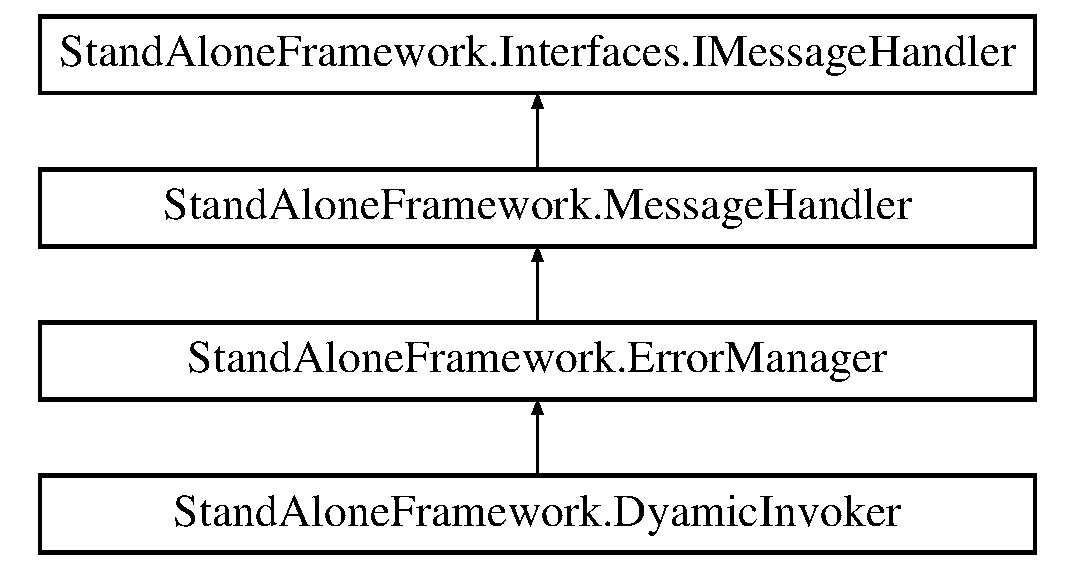
\includegraphics[height=4.000000cm]{interface_stand_alone_framework_1_1_interfaces_1_1_i_message_handler}
\end{center}
\end{figure}


The documentation for this interface was generated from the following file\+:\begin{DoxyCompactItemize}
\item 
C\+:/\+Users/\+Charles Trent Spare/\+Documents/\+Source Control/\+Repositories/\+Development\+Projects/\+Stand\+Alone\+Framework/\+Stand\+Alone\+Framework/\+Message\+Handler/\+Interfaces/\hyperlink{_i_message_handler_8cs}{I\+Message\+Handler.\+cs}\end{DoxyCompactItemize}

\hypertarget{interface_stand_alone_framework_1_1_method_facade_1_1_interfaces_1_1_i_method_facade}{\section{Stand\+Alone\+Framework.\+Method\+Facade.\+Interfaces.\+I\+Method\+Facade Interface Reference}
\label{interface_stand_alone_framework_1_1_method_facade_1_1_interfaces_1_1_i_method_facade}\index{Stand\+Alone\+Framework.\+Method\+Facade.\+Interfaces.\+I\+Method\+Facade@{Stand\+Alone\+Framework.\+Method\+Facade.\+Interfaces.\+I\+Method\+Facade}}
}


The \hyperlink{class_stand_alone_framework_1_1_method_facade_1_1_method_facade}{Method\+Facade} contract  


Inheritance diagram for Stand\+Alone\+Framework.\+Method\+Facade.\+Interfaces.\+I\+Method\+Facade\+:\begin{figure}[H]
\begin{center}
\leavevmode
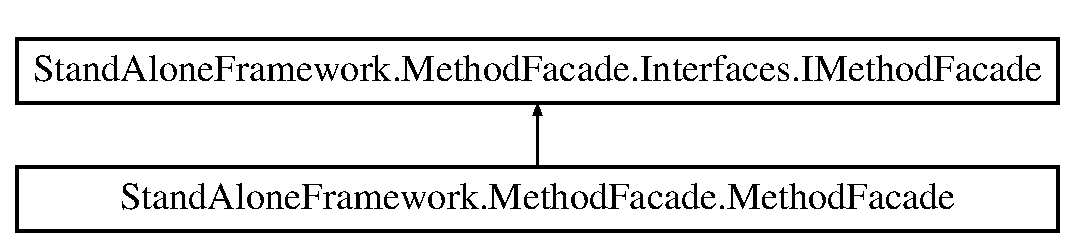
\includegraphics[height=2.000000cm]{interface_stand_alone_framework_1_1_method_facade_1_1_interfaces_1_1_i_method_facade}
\end{center}
\end{figure}


\subsection{Detailed Description}
The \hyperlink{class_stand_alone_framework_1_1_method_facade_1_1_method_facade}{Method\+Facade} contract 



The documentation for this interface was generated from the following file\+:\begin{DoxyCompactItemize}
\item 
C\+:/\+Users/\+Charles Trent Spare/\+Documents/\+Source Control/\+Repositories/\+Development\+Projects/\+Stand\+Alone\+Framework/\+Stand\+Alone\+Framework/\+Method\+Facade/\+Interfaces/\hyperlink{_i_method_facade_8cs}{I\+Method\+Facade.\+cs}\end{DoxyCompactItemize}

\hypertarget{interface_stand_alone_framework_1_1_factories_1_1_interfaces_1_1_i_method_factory}{\section{Stand\+Alone\+Framework.\+Factories.\+Interfaces.\+I\+Method\+Factory Interface Reference}
\label{interface_stand_alone_framework_1_1_factories_1_1_interfaces_1_1_i_method_factory}\index{Stand\+Alone\+Framework.\+Factories.\+Interfaces.\+I\+Method\+Factory@{Stand\+Alone\+Framework.\+Factories.\+Interfaces.\+I\+Method\+Factory}}
}
Inheritance diagram for Stand\+Alone\+Framework.\+Factories.\+Interfaces.\+I\+Method\+Factory\+:\begin{figure}[H]
\begin{center}
\leavevmode
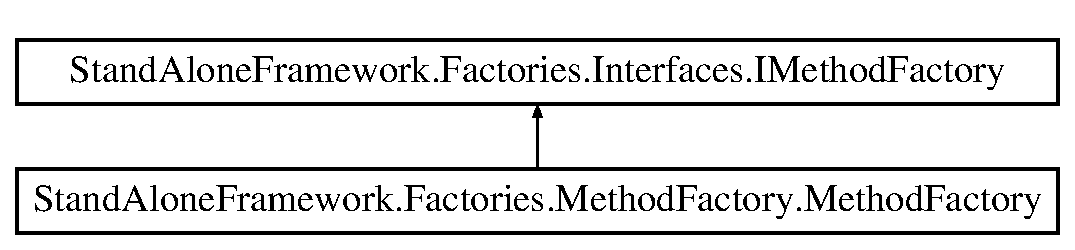
\includegraphics[height=2.000000cm]{interface_stand_alone_framework_1_1_factories_1_1_interfaces_1_1_i_method_factory}
\end{center}
\end{figure}
\subsection*{Public Member Functions}
\begin{DoxyCompactItemize}
\item 
object \hyperlink{interface_stand_alone_framework_1_1_factories_1_1_interfaces_1_1_i_method_factory_a699e7a06cdb746034ce0d7b38d9cf21c}{Execute\+Method} ()
\item 
void \hyperlink{interface_stand_alone_framework_1_1_factories_1_1_interfaces_1_1_i_method_factory_aafd802da0b25eaf9e11c53b9c0d06bdf}{Start\+Factory} (\hyperlink{namespace_stand_alone_framework_1_1_factories_1_1_method_factory_a03ffbf0d8e733b86d0ac29ae38dd4241}{Method\+Return\+Type} method\+Return\+Type, \hyperlink{namespace_stand_alone_framework_1_1_factories_1_1_method_factory_aeb6e05dc016e73b072faae5a5d275f6a}{Method\+Type} method\+Type, \hyperlink{namespace_stand_alone_framework_1_1_factories_1_1_thread_factory_aaa02326f96ee10b7d0fd360488d27c39}{Threading\+Model} threading\+Model, object method\+To\+Invoke, \hyperlink{class_stand_alone_framework_1_1_data_wrapper}{Data\+Wrapper} args)
\end{DoxyCompactItemize}
\subsection*{Properties}
\begin{DoxyCompactItemize}
\item 
\hyperlink{interface_stand_alone_framework_1_1_factories_1_1_interfaces_1_1_i_thread_factory}{I\+Thread\+Factory} \hyperlink{interface_stand_alone_framework_1_1_factories_1_1_interfaces_1_1_i_method_factory_ac06213a945419bd5e1b34450410069a1}{Thread\+Factory}\hspace{0.3cm}{\ttfamily  \mbox{[}get, set\mbox{]}}
\item 
\hyperlink{class_stand_alone_framework_1_1_factories_1_1_method_factory_1_1_method_wrapper}{Method\+Wrapper} \hyperlink{interface_stand_alone_framework_1_1_factories_1_1_interfaces_1_1_i_method_factory_a2390dfd96f153491c70db92ff7e1b9e3}{Method\+Wrapper}\hspace{0.3cm}{\ttfamily  \mbox{[}get, set\mbox{]}}
\end{DoxyCompactItemize}


\subsection{Member Function Documentation}
\hypertarget{interface_stand_alone_framework_1_1_factories_1_1_interfaces_1_1_i_method_factory_a699e7a06cdb746034ce0d7b38d9cf21c}{\index{Stand\+Alone\+Framework\+::\+Factories\+::\+Interfaces\+::\+I\+Method\+Factory@{Stand\+Alone\+Framework\+::\+Factories\+::\+Interfaces\+::\+I\+Method\+Factory}!Execute\+Method@{Execute\+Method}}
\index{Execute\+Method@{Execute\+Method}!Stand\+Alone\+Framework\+::\+Factories\+::\+Interfaces\+::\+I\+Method\+Factory@{Stand\+Alone\+Framework\+::\+Factories\+::\+Interfaces\+::\+I\+Method\+Factory}}
\subsubsection[{Execute\+Method}]{\setlength{\rightskip}{0pt plus 5cm}object Stand\+Alone\+Framework.\+Factories.\+Interfaces.\+I\+Method\+Factory.\+Execute\+Method (
\begin{DoxyParamCaption}
{}
\end{DoxyParamCaption}
)}}\label{interface_stand_alone_framework_1_1_factories_1_1_interfaces_1_1_i_method_factory_a699e7a06cdb746034ce0d7b38d9cf21c}


Implemented in \hyperlink{class_stand_alone_framework_1_1_factories_1_1_method_factory_1_1_method_factory_a5e1c85f6928f23809770682565ce18ef}{Stand\+Alone\+Framework.\+Factories.\+Method\+Factory.\+Method\+Factory}.

\hypertarget{interface_stand_alone_framework_1_1_factories_1_1_interfaces_1_1_i_method_factory_aafd802da0b25eaf9e11c53b9c0d06bdf}{\index{Stand\+Alone\+Framework\+::\+Factories\+::\+Interfaces\+::\+I\+Method\+Factory@{Stand\+Alone\+Framework\+::\+Factories\+::\+Interfaces\+::\+I\+Method\+Factory}!Start\+Factory@{Start\+Factory}}
\index{Start\+Factory@{Start\+Factory}!Stand\+Alone\+Framework\+::\+Factories\+::\+Interfaces\+::\+I\+Method\+Factory@{Stand\+Alone\+Framework\+::\+Factories\+::\+Interfaces\+::\+I\+Method\+Factory}}
\subsubsection[{Start\+Factory}]{\setlength{\rightskip}{0pt plus 5cm}void Stand\+Alone\+Framework.\+Factories.\+Interfaces.\+I\+Method\+Factory.\+Start\+Factory (
\begin{DoxyParamCaption}
\item[{{\bf Method\+Return\+Type}}]{method\+Return\+Type, }
\item[{{\bf Method\+Type}}]{method\+Type, }
\item[{{\bf Threading\+Model}}]{threading\+Model, }
\item[{object}]{method\+To\+Invoke, }
\item[{{\bf Data\+Wrapper}}]{args}
\end{DoxyParamCaption}
)}}\label{interface_stand_alone_framework_1_1_factories_1_1_interfaces_1_1_i_method_factory_aafd802da0b25eaf9e11c53b9c0d06bdf}


Implemented in \hyperlink{class_stand_alone_framework_1_1_factories_1_1_method_factory_1_1_method_factory_ad7266b9459d17e8931b267470a3f65a3}{Stand\+Alone\+Framework.\+Factories.\+Method\+Factory.\+Method\+Factory}.



\subsection{Property Documentation}
\hypertarget{interface_stand_alone_framework_1_1_factories_1_1_interfaces_1_1_i_method_factory_a2390dfd96f153491c70db92ff7e1b9e3}{\index{Stand\+Alone\+Framework\+::\+Factories\+::\+Interfaces\+::\+I\+Method\+Factory@{Stand\+Alone\+Framework\+::\+Factories\+::\+Interfaces\+::\+I\+Method\+Factory}!Method\+Wrapper@{Method\+Wrapper}}
\index{Method\+Wrapper@{Method\+Wrapper}!Stand\+Alone\+Framework\+::\+Factories\+::\+Interfaces\+::\+I\+Method\+Factory@{Stand\+Alone\+Framework\+::\+Factories\+::\+Interfaces\+::\+I\+Method\+Factory}}
\subsubsection[{Method\+Wrapper}]{\setlength{\rightskip}{0pt plus 5cm}{\bf Method\+Wrapper} Stand\+Alone\+Framework.\+Factories.\+Interfaces.\+I\+Method\+Factory.\+Method\+Wrapper\hspace{0.3cm}{\ttfamily [get]}, {\ttfamily [set]}}}\label{interface_stand_alone_framework_1_1_factories_1_1_interfaces_1_1_i_method_factory_a2390dfd96f153491c70db92ff7e1b9e3}
\hypertarget{interface_stand_alone_framework_1_1_factories_1_1_interfaces_1_1_i_method_factory_ac06213a945419bd5e1b34450410069a1}{\index{Stand\+Alone\+Framework\+::\+Factories\+::\+Interfaces\+::\+I\+Method\+Factory@{Stand\+Alone\+Framework\+::\+Factories\+::\+Interfaces\+::\+I\+Method\+Factory}!Thread\+Factory@{Thread\+Factory}}
\index{Thread\+Factory@{Thread\+Factory}!Stand\+Alone\+Framework\+::\+Factories\+::\+Interfaces\+::\+I\+Method\+Factory@{Stand\+Alone\+Framework\+::\+Factories\+::\+Interfaces\+::\+I\+Method\+Factory}}
\subsubsection[{Thread\+Factory}]{\setlength{\rightskip}{0pt plus 5cm}{\bf I\+Thread\+Factory} Stand\+Alone\+Framework.\+Factories.\+Interfaces.\+I\+Method\+Factory.\+Thread\+Factory\hspace{0.3cm}{\ttfamily [get]}, {\ttfamily [set]}}}\label{interface_stand_alone_framework_1_1_factories_1_1_interfaces_1_1_i_method_factory_ac06213a945419bd5e1b34450410069a1}


The documentation for this interface was generated from the following file\+:\begin{DoxyCompactItemize}
\item 
C\+:/\+Users/\+Charles Trent Spare/\+Documents/\+Source Control/\+Repositories/\+Development\+Projects/\+Stand\+Alone\+Framework/\+Stand\+Alone\+Framework/\+Factories/\+Method\+Factory/\+Interfaces/\hyperlink{_i_method_factory_8cs}{I\+Method\+Factory.\+cs}\end{DoxyCompactItemize}

\hypertarget{class_stand_alone_framework_1_1_framework_classes_1_1_invocation_result}{\section{Stand\+Alone\+Framework.\+Framework\+Classes.\+Invocation\+Result Class Reference}
\label{class_stand_alone_framework_1_1_framework_classes_1_1_invocation_result}\index{Stand\+Alone\+Framework.\+Framework\+Classes.\+Invocation\+Result@{Stand\+Alone\+Framework.\+Framework\+Classes.\+Invocation\+Result}}
}


Encapsulates the return values of the method execution. The return values could contain contain any error messages, data that is returned from the method execution  


Inheritance diagram for Stand\+Alone\+Framework.\+Framework\+Classes.\+Invocation\+Result\+:\begin{figure}[H]
\begin{center}
\leavevmode
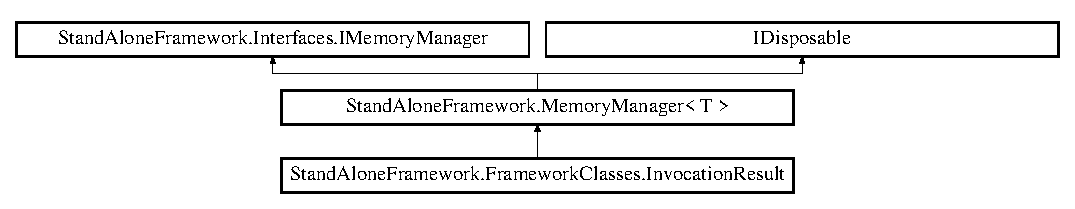
\includegraphics[height=2.366197cm]{class_stand_alone_framework_1_1_framework_classes_1_1_invocation_result}
\end{center}
\end{figure}
\subsection*{Public Types}
\begin{DoxyCompactItemize}
\item 
enum \hyperlink{class_stand_alone_framework_1_1_framework_classes_1_1_invocation_result_a536bbf61143c8a5b8364bf7c77896ba4}{Invocation\+Result\+Type} \{ \hyperlink{class_stand_alone_framework_1_1_framework_classes_1_1_invocation_result_a536bbf61143c8a5b8364bf7c77896ba4a902b0d55fddef6f8d651fe1035b7d4bd}{Invocation\+Result\+Type.\+Error}, 
\hyperlink{class_stand_alone_framework_1_1_framework_classes_1_1_invocation_result_a536bbf61143c8a5b8364bf7c77896ba4a505a83f220c02df2f85c3810cd9ceb38}{Invocation\+Result\+Type.\+Success}
 \}
\begin{DoxyCompactList}\small\item\em Represents the execution result type \end{DoxyCompactList}\end{DoxyCompactItemize}
\subsection*{Properties}
\begin{DoxyCompactItemize}
\item 
string \hyperlink{class_stand_alone_framework_1_1_framework_classes_1_1_invocation_result_a901421598cda8841d37a774865e7d037}{Message}\hspace{0.3cm}{\ttfamily  \mbox{[}get, set\mbox{]}}
\begin{DoxyCompactList}\small\item\em Gets or sets the friendly error message. \end{DoxyCompactList}\item 
\hyperlink{class_stand_alone_framework_1_1_framework_classes_1_1_invocation_result_a536bbf61143c8a5b8364bf7c77896ba4}{Invocation\+Result\+Type} \hyperlink{class_stand_alone_framework_1_1_framework_classes_1_1_invocation_result_a581f41c7d799d0ea4eb63660cc901b7c}{Message\+Type}\hspace{0.3cm}{\ttfamily  \mbox{[}get, set\mbox{]}}
\begin{DoxyCompactList}\small\item\em Gets or sets the type of the message. \end{DoxyCompactList}\item 
object \hyperlink{class_stand_alone_framework_1_1_framework_classes_1_1_invocation_result_a3cd591d332da9a4149dfa2444cec747e}{Data}\hspace{0.3cm}{\ttfamily  \mbox{[}get, set\mbox{]}}
\begin{DoxyCompactList}\small\item\em Gets or sets the data that is returned from the method execution. \end{DoxyCompactList}\end{DoxyCompactItemize}
\subsection*{Additional Inherited Members}


\subsection{Detailed Description}
Encapsulates the return values of the method execution. The return values could contain contain any error messages, data that is returned from the method execution 



\subsection{Member Enumeration Documentation}
\hypertarget{class_stand_alone_framework_1_1_framework_classes_1_1_invocation_result_a536bbf61143c8a5b8364bf7c77896ba4}{\index{Stand\+Alone\+Framework\+::\+Framework\+Classes\+::\+Invocation\+Result@{Stand\+Alone\+Framework\+::\+Framework\+Classes\+::\+Invocation\+Result}!Invocation\+Result\+Type@{Invocation\+Result\+Type}}
\index{Invocation\+Result\+Type@{Invocation\+Result\+Type}!Stand\+Alone\+Framework\+::\+Framework\+Classes\+::\+Invocation\+Result@{Stand\+Alone\+Framework\+::\+Framework\+Classes\+::\+Invocation\+Result}}
\subsubsection[{Invocation\+Result\+Type}]{\setlength{\rightskip}{0pt plus 5cm}enum {\bf Stand\+Alone\+Framework.\+Framework\+Classes.\+Invocation\+Result.\+Invocation\+Result\+Type}}}\label{class_stand_alone_framework_1_1_framework_classes_1_1_invocation_result_a536bbf61143c8a5b8364bf7c77896ba4}


Represents the execution result type 

\begin{Desc}
\item[Enumerator]\par
\begin{description}
\index{Error@{Error}!Stand\+Alone\+Framework\+::\+Framework\+Classes\+::\+Invocation\+Result@{Stand\+Alone\+Framework\+::\+Framework\+Classes\+::\+Invocation\+Result}}\index{Stand\+Alone\+Framework\+::\+Framework\+Classes\+::\+Invocation\+Result@{Stand\+Alone\+Framework\+::\+Framework\+Classes\+::\+Invocation\+Result}!Error@{Error}}\item[{\em 
\hypertarget{class_stand_alone_framework_1_1_framework_classes_1_1_invocation_result_a536bbf61143c8a5b8364bf7c77896ba4a902b0d55fddef6f8d651fe1035b7d4bd}{Error}\label{class_stand_alone_framework_1_1_framework_classes_1_1_invocation_result_a536bbf61143c8a5b8364bf7c77896ba4a902b0d55fddef6f8d651fe1035b7d4bd}
}]An error occurred during method execution \index{Success@{Success}!Stand\+Alone\+Framework\+::\+Framework\+Classes\+::\+Invocation\+Result@{Stand\+Alone\+Framework\+::\+Framework\+Classes\+::\+Invocation\+Result}}\index{Stand\+Alone\+Framework\+::\+Framework\+Classes\+::\+Invocation\+Result@{Stand\+Alone\+Framework\+::\+Framework\+Classes\+::\+Invocation\+Result}!Success@{Success}}\item[{\em 
\hypertarget{class_stand_alone_framework_1_1_framework_classes_1_1_invocation_result_a536bbf61143c8a5b8364bf7c77896ba4a505a83f220c02df2f85c3810cd9ceb38}{Success}\label{class_stand_alone_framework_1_1_framework_classes_1_1_invocation_result_a536bbf61143c8a5b8364bf7c77896ba4a505a83f220c02df2f85c3810cd9ceb38}
}]No errors occurred during method execution \end{description}
\end{Desc}


\subsection{Property Documentation}
\hypertarget{class_stand_alone_framework_1_1_framework_classes_1_1_invocation_result_a3cd591d332da9a4149dfa2444cec747e}{\index{Stand\+Alone\+Framework\+::\+Framework\+Classes\+::\+Invocation\+Result@{Stand\+Alone\+Framework\+::\+Framework\+Classes\+::\+Invocation\+Result}!Data@{Data}}
\index{Data@{Data}!Stand\+Alone\+Framework\+::\+Framework\+Classes\+::\+Invocation\+Result@{Stand\+Alone\+Framework\+::\+Framework\+Classes\+::\+Invocation\+Result}}
\subsubsection[{Data}]{\setlength{\rightskip}{0pt plus 5cm}object Stand\+Alone\+Framework.\+Framework\+Classes.\+Invocation\+Result.\+Data\hspace{0.3cm}{\ttfamily [get]}, {\ttfamily [set]}}}\label{class_stand_alone_framework_1_1_framework_classes_1_1_invocation_result_a3cd591d332da9a4149dfa2444cec747e}


Gets or sets the data that is returned from the method execution. 

The data.\hypertarget{class_stand_alone_framework_1_1_framework_classes_1_1_invocation_result_a901421598cda8841d37a774865e7d037}{\index{Stand\+Alone\+Framework\+::\+Framework\+Classes\+::\+Invocation\+Result@{Stand\+Alone\+Framework\+::\+Framework\+Classes\+::\+Invocation\+Result}!Message@{Message}}
\index{Message@{Message}!Stand\+Alone\+Framework\+::\+Framework\+Classes\+::\+Invocation\+Result@{Stand\+Alone\+Framework\+::\+Framework\+Classes\+::\+Invocation\+Result}}
\subsubsection[{Message}]{\setlength{\rightskip}{0pt plus 5cm}string Stand\+Alone\+Framework.\+Framework\+Classes.\+Invocation\+Result.\+Message\hspace{0.3cm}{\ttfamily [get]}, {\ttfamily [set]}}}\label{class_stand_alone_framework_1_1_framework_classes_1_1_invocation_result_a901421598cda8841d37a774865e7d037}


Gets or sets the friendly error message. 

The message.\hypertarget{class_stand_alone_framework_1_1_framework_classes_1_1_invocation_result_a581f41c7d799d0ea4eb63660cc901b7c}{\index{Stand\+Alone\+Framework\+::\+Framework\+Classes\+::\+Invocation\+Result@{Stand\+Alone\+Framework\+::\+Framework\+Classes\+::\+Invocation\+Result}!Message\+Type@{Message\+Type}}
\index{Message\+Type@{Message\+Type}!Stand\+Alone\+Framework\+::\+Framework\+Classes\+::\+Invocation\+Result@{Stand\+Alone\+Framework\+::\+Framework\+Classes\+::\+Invocation\+Result}}
\subsubsection[{Message\+Type}]{\setlength{\rightskip}{0pt plus 5cm}{\bf Invocation\+Result\+Type} Stand\+Alone\+Framework.\+Framework\+Classes.\+Invocation\+Result.\+Message\+Type\hspace{0.3cm}{\ttfamily [get]}, {\ttfamily [set]}}}\label{class_stand_alone_framework_1_1_framework_classes_1_1_invocation_result_a581f41c7d799d0ea4eb63660cc901b7c}


Gets or sets the type of the message. 

The type of the message.

The documentation for this class was generated from the following file\+:\begin{DoxyCompactItemize}
\item 
C\+:/\+Users/\+Charles Trent Spare/\+Documents/\+Source Control/\+Repositories/\+Development\+Projects/\+Stand\+Alone\+Framework/\+Stand\+Alone\+Framework/\+Framework\+Classes/\hyperlink{_invocation_result_8cs}{Invocation\+Result.\+cs}\end{DoxyCompactItemize}

\hypertarget{interface_stand_alone_framework_1_1_factories_1_1_interfaces_1_1_i_thread_factory}{\section{Stand\+Alone\+Framework.\+Factories.\+Interfaces.\+I\+Thread\+Factory Interface Reference}
\label{interface_stand_alone_framework_1_1_factories_1_1_interfaces_1_1_i_thread_factory}\index{Stand\+Alone\+Framework.\+Factories.\+Interfaces.\+I\+Thread\+Factory@{Stand\+Alone\+Framework.\+Factories.\+Interfaces.\+I\+Thread\+Factory}}
}


The \hyperlink{namespace_stand_alone_framework_1_1_factories_1_1_thread_factory}{Thread\+Factory} contract  


Inheritance diagram for Stand\+Alone\+Framework.\+Factories.\+Interfaces.\+I\+Thread\+Factory\+:\begin{figure}[H]
\begin{center}
\leavevmode
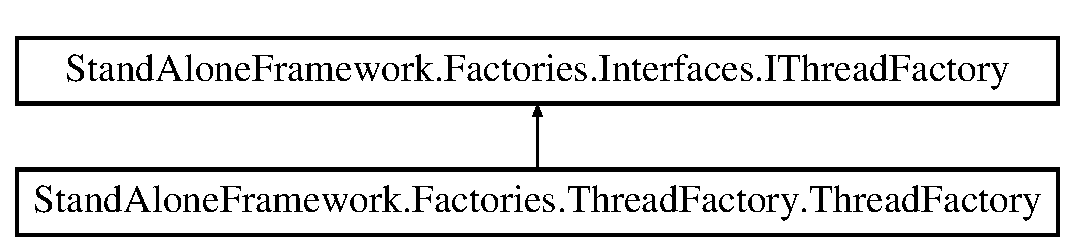
\includegraphics[height=2.000000cm]{interface_stand_alone_framework_1_1_factories_1_1_interfaces_1_1_i_thread_factory}
\end{center}
\end{figure}
\subsection*{Public Member Functions}
\begin{DoxyCompactItemize}
\item 
void \hyperlink{interface_stand_alone_framework_1_1_factories_1_1_interfaces_1_1_i_thread_factory_aa57ffdc6e7234b5377bfc4bdc319f985}{Create\+Thread} (\hyperlink{class_stand_alone_framework_1_1_factories_1_1_method_factory_1_1_method_wrapper}{Method\+Wrapper} threading\+Model)
\begin{DoxyCompactList}\small\item\em Creates the thread for the current method call. \end{DoxyCompactList}\item 
Thread \hyperlink{interface_stand_alone_framework_1_1_factories_1_1_interfaces_1_1_i_thread_factory_a6a9c8007ba1e6738f7013089f1f9117c}{Find\+Thread} (int thread\+Id)
\begin{DoxyCompactList}\small\item\em Finds the thread for the specific thread id. \end{DoxyCompactList}\end{DoxyCompactItemize}
\subsection*{Properties}
\begin{DoxyCompactItemize}
\item 
I\+List$<$ Thread $>$ \hyperlink{interface_stand_alone_framework_1_1_factories_1_1_interfaces_1_1_i_thread_factory_a51adc616b01dc8db654da67f200fa394}{Running\+Threads}\hspace{0.3cm}{\ttfamily  \mbox{[}get, set\mbox{]}}
\begin{DoxyCompactList}\small\item\em Gets or sets the running threads in the current method call. \end{DoxyCompactList}\end{DoxyCompactItemize}


\subsection{Detailed Description}
The \hyperlink{namespace_stand_alone_framework_1_1_factories_1_1_thread_factory}{Thread\+Factory} contract 



\subsection{Member Function Documentation}
\hypertarget{interface_stand_alone_framework_1_1_factories_1_1_interfaces_1_1_i_thread_factory_aa57ffdc6e7234b5377bfc4bdc319f985}{\index{Stand\+Alone\+Framework\+::\+Factories\+::\+Interfaces\+::\+I\+Thread\+Factory@{Stand\+Alone\+Framework\+::\+Factories\+::\+Interfaces\+::\+I\+Thread\+Factory}!Create\+Thread@{Create\+Thread}}
\index{Create\+Thread@{Create\+Thread}!Stand\+Alone\+Framework\+::\+Factories\+::\+Interfaces\+::\+I\+Thread\+Factory@{Stand\+Alone\+Framework\+::\+Factories\+::\+Interfaces\+::\+I\+Thread\+Factory}}
\subsubsection[{Create\+Thread}]{\setlength{\rightskip}{0pt plus 5cm}void Stand\+Alone\+Framework.\+Factories.\+Interfaces.\+I\+Thread\+Factory.\+Create\+Thread (
\begin{DoxyParamCaption}
\item[{{\bf Method\+Wrapper}}]{threading\+Model}
\end{DoxyParamCaption}
)}}\label{interface_stand_alone_framework_1_1_factories_1_1_interfaces_1_1_i_thread_factory_aa57ffdc6e7234b5377bfc4bdc319f985}


Creates the thread for the current method call. 


\begin{DoxyParams}{Parameters}
{\em threading\+Model} & The threading model.\\
\hline
\end{DoxyParams}


Implemented in \hyperlink{class_stand_alone_framework_1_1_factories_1_1_thread_factory_1_1_thread_factory_a4fb8eb961ebeb6acfbaab63f169a1cb8}{Stand\+Alone\+Framework.\+Factories.\+Thread\+Factory.\+Thread\+Factory}.

\hypertarget{interface_stand_alone_framework_1_1_factories_1_1_interfaces_1_1_i_thread_factory_a6a9c8007ba1e6738f7013089f1f9117c}{\index{Stand\+Alone\+Framework\+::\+Factories\+::\+Interfaces\+::\+I\+Thread\+Factory@{Stand\+Alone\+Framework\+::\+Factories\+::\+Interfaces\+::\+I\+Thread\+Factory}!Find\+Thread@{Find\+Thread}}
\index{Find\+Thread@{Find\+Thread}!Stand\+Alone\+Framework\+::\+Factories\+::\+Interfaces\+::\+I\+Thread\+Factory@{Stand\+Alone\+Framework\+::\+Factories\+::\+Interfaces\+::\+I\+Thread\+Factory}}
\subsubsection[{Find\+Thread}]{\setlength{\rightskip}{0pt plus 5cm}Thread Stand\+Alone\+Framework.\+Factories.\+Interfaces.\+I\+Thread\+Factory.\+Find\+Thread (
\begin{DoxyParamCaption}
\item[{int}]{thread\+Id}
\end{DoxyParamCaption}
)}}\label{interface_stand_alone_framework_1_1_factories_1_1_interfaces_1_1_i_thread_factory_a6a9c8007ba1e6738f7013089f1f9117c}


Finds the thread for the specific thread id. 


\begin{DoxyParams}{Parameters}
{\em thread\+Id} & The thread identifier.\\
\hline
\end{DoxyParams}
\begin{DoxyReturn}{Returns}
Thread.
\end{DoxyReturn}


Implemented in \hyperlink{class_stand_alone_framework_1_1_factories_1_1_thread_factory_1_1_thread_factory_a19b01caebe842de7e8ac8989319af582}{Stand\+Alone\+Framework.\+Factories.\+Thread\+Factory.\+Thread\+Factory}.



\subsection{Property Documentation}
\hypertarget{interface_stand_alone_framework_1_1_factories_1_1_interfaces_1_1_i_thread_factory_a51adc616b01dc8db654da67f200fa394}{\index{Stand\+Alone\+Framework\+::\+Factories\+::\+Interfaces\+::\+I\+Thread\+Factory@{Stand\+Alone\+Framework\+::\+Factories\+::\+Interfaces\+::\+I\+Thread\+Factory}!Running\+Threads@{Running\+Threads}}
\index{Running\+Threads@{Running\+Threads}!Stand\+Alone\+Framework\+::\+Factories\+::\+Interfaces\+::\+I\+Thread\+Factory@{Stand\+Alone\+Framework\+::\+Factories\+::\+Interfaces\+::\+I\+Thread\+Factory}}
\subsubsection[{Running\+Threads}]{\setlength{\rightskip}{0pt plus 5cm}I\+List$<$Thread$>$ Stand\+Alone\+Framework.\+Factories.\+Interfaces.\+I\+Thread\+Factory.\+Running\+Threads\hspace{0.3cm}{\ttfamily [get]}, {\ttfamily [set]}}}\label{interface_stand_alone_framework_1_1_factories_1_1_interfaces_1_1_i_thread_factory_a51adc616b01dc8db654da67f200fa394}


Gets or sets the running threads in the current method call. 

The running threads.

The documentation for this interface was generated from the following file\+:\begin{DoxyCompactItemize}
\item 
C\+:/\+Users/\+Charles Trent Spare/\+Documents/\+Source Control/\+Repositories/\+Development\+Projects/\+Stand\+Alone\+Framework/\+Stand\+Alone\+Framework/\+Factories/\+Thread\+Factory/\+Interfaces/\hyperlink{_i_thread_factory_8cs}{I\+Thread\+Factory.\+cs}\end{DoxyCompactItemize}

\hypertarget{class_stand_alone_framework_1_1_memory_manager_3_01_t_01_4}{\section{Stand\+Alone\+Framework.\+Memory\+Manager$<$ T $>$ Class Template Reference}
\label{class_stand_alone_framework_1_1_memory_manager_3_01_t_01_4}\index{Stand\+Alone\+Framework.\+Memory\+Manager$<$ T $>$@{Stand\+Alone\+Framework.\+Memory\+Manager$<$ T $>$}}
}


Represents the memory manager that active manages the lifetime of any object that derives from it  


Inheritance diagram for Stand\+Alone\+Framework.\+Memory\+Manager$<$ T $>$\+:\begin{figure}[H]
\begin{center}
\leavevmode
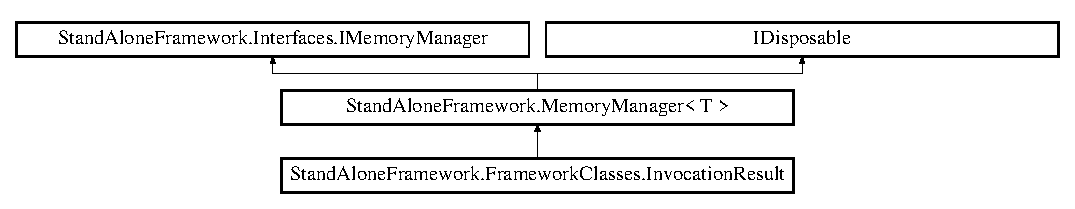
\includegraphics[height=2.366197cm]{class_stand_alone_framework_1_1_memory_manager_3_01_t_01_4}
\end{center}
\end{figure}
\subsection*{Public Member Functions}
\begin{DoxyCompactItemize}
\item 
void \hyperlink{class_stand_alone_framework_1_1_memory_manager_3_01_t_01_4_a1efb4ab4f0a190ef25a13b2aaf524267}{Dispose} ()
\begin{DoxyCompactList}\small\item\em Performs application-\/defined tasks associated with freeing, releasing, or resetting unmanaged resources. \end{DoxyCompactList}\item 
void \hyperlink{class_stand_alone_framework_1_1_memory_manager_3_01_t_01_4_ad7aee15edbfecdb55eee947874a8c4cd}{Dispose\+Object} (object instance)
\begin{DoxyCompactList}\small\item\em Disposes the object. \end{DoxyCompactList}\end{DoxyCompactItemize}
\subsection*{Protected Member Functions}
\begin{DoxyCompactItemize}
\item 
virtual void \hyperlink{class_stand_alone_framework_1_1_memory_manager_3_01_t_01_4_a52f69219ea9d645b8246e27b0a82a0a3}{Dispose} (bool disposing)
\begin{DoxyCompactList}\small\item\em Releases unmanaged and -\/ optionally -\/ managed resources. \end{DoxyCompactList}\end{DoxyCompactItemize}
\subsection*{Properties}
\begin{DoxyCompactItemize}
\item 
bool \hyperlink{class_stand_alone_framework_1_1_memory_manager_3_01_t_01_4_ad2375b894216a59e50c1942ee82f41c6}{Is\+Object\+Disposed}\hspace{0.3cm}{\ttfamily  \mbox{[}get, set\mbox{]}}
\begin{DoxyCompactList}\small\item\em Gets or sets a value indicating whether this instance of the object disposed. \end{DoxyCompactList}\end{DoxyCompactItemize}


\subsection{Detailed Description}
Represents the memory manager that active manages the lifetime of any object that derives from it 


\begin{DoxyTemplParams}{Template Parameters}
{\em T} & \\
\hline
\end{DoxyTemplParams}


\subsection{Member Function Documentation}
\hypertarget{class_stand_alone_framework_1_1_memory_manager_3_01_t_01_4_a1efb4ab4f0a190ef25a13b2aaf524267}{\index{Stand\+Alone\+Framework\+::\+Memory\+Manager$<$ T $>$@{Stand\+Alone\+Framework\+::\+Memory\+Manager$<$ T $>$}!Dispose@{Dispose}}
\index{Dispose@{Dispose}!Stand\+Alone\+Framework\+::\+Memory\+Manager$<$ T $>$@{Stand\+Alone\+Framework\+::\+Memory\+Manager$<$ T $>$}}
\subsubsection[{Dispose}]{\setlength{\rightskip}{0pt plus 5cm}void Stand\+Alone\+Framework.\+Memory\+Manager$<$ T $>$.Dispose (
\begin{DoxyParamCaption}
{}
\end{DoxyParamCaption}
)}}\label{class_stand_alone_framework_1_1_memory_manager_3_01_t_01_4_a1efb4ab4f0a190ef25a13b2aaf524267}


Performs application-\/defined tasks associated with freeing, releasing, or resetting unmanaged resources. 

\hypertarget{class_stand_alone_framework_1_1_memory_manager_3_01_t_01_4_a52f69219ea9d645b8246e27b0a82a0a3}{\index{Stand\+Alone\+Framework\+::\+Memory\+Manager$<$ T $>$@{Stand\+Alone\+Framework\+::\+Memory\+Manager$<$ T $>$}!Dispose@{Dispose}}
\index{Dispose@{Dispose}!Stand\+Alone\+Framework\+::\+Memory\+Manager$<$ T $>$@{Stand\+Alone\+Framework\+::\+Memory\+Manager$<$ T $>$}}
\subsubsection[{Dispose}]{\setlength{\rightskip}{0pt plus 5cm}virtual void Stand\+Alone\+Framework.\+Memory\+Manager$<$ T $>$.Dispose (
\begin{DoxyParamCaption}
\item[{bool}]{disposing}
\end{DoxyParamCaption}
)\hspace{0.3cm}{\ttfamily [protected]}, {\ttfamily [virtual]}}}\label{class_stand_alone_framework_1_1_memory_manager_3_01_t_01_4_a52f69219ea9d645b8246e27b0a82a0a3}


Releases unmanaged and -\/ optionally -\/ managed resources. 


\begin{DoxyParams}{Parameters}
{\em disposing} & {\ttfamily true} to release both managed and unmanaged resources; {\ttfamily false} to release only unmanaged resources.\\
\hline
\end{DoxyParams}
\hypertarget{class_stand_alone_framework_1_1_memory_manager_3_01_t_01_4_ad7aee15edbfecdb55eee947874a8c4cd}{\index{Stand\+Alone\+Framework\+::\+Memory\+Manager$<$ T $>$@{Stand\+Alone\+Framework\+::\+Memory\+Manager$<$ T $>$}!Dispose\+Object@{Dispose\+Object}}
\index{Dispose\+Object@{Dispose\+Object}!Stand\+Alone\+Framework\+::\+Memory\+Manager$<$ T $>$@{Stand\+Alone\+Framework\+::\+Memory\+Manager$<$ T $>$}}
\subsubsection[{Dispose\+Object}]{\setlength{\rightskip}{0pt plus 5cm}void Stand\+Alone\+Framework.\+Memory\+Manager$<$ T $>$.Dispose\+Object (
\begin{DoxyParamCaption}
\item[{object}]{instance}
\end{DoxyParamCaption}
)}}\label{class_stand_alone_framework_1_1_memory_manager_3_01_t_01_4_ad7aee15edbfecdb55eee947874a8c4cd}


Disposes the object. 


\begin{DoxyParams}{Parameters}
{\em instance} & The instance.\\
\hline
\end{DoxyParams}


Implements \hyperlink{interface_stand_alone_framework_1_1_interfaces_1_1_i_memory_manager_a277ad312644179fa202782319ee5e801}{Stand\+Alone\+Framework.\+Interfaces.\+I\+Memory\+Manager}.



\subsection{Property Documentation}
\hypertarget{class_stand_alone_framework_1_1_memory_manager_3_01_t_01_4_ad2375b894216a59e50c1942ee82f41c6}{\index{Stand\+Alone\+Framework\+::\+Memory\+Manager$<$ T $>$@{Stand\+Alone\+Framework\+::\+Memory\+Manager$<$ T $>$}!Is\+Object\+Disposed@{Is\+Object\+Disposed}}
\index{Is\+Object\+Disposed@{Is\+Object\+Disposed}!Stand\+Alone\+Framework\+::\+Memory\+Manager$<$ T $>$@{Stand\+Alone\+Framework\+::\+Memory\+Manager$<$ T $>$}}
\subsubsection[{Is\+Object\+Disposed}]{\setlength{\rightskip}{0pt plus 5cm}bool Stand\+Alone\+Framework.\+Memory\+Manager$<$ T $>$.Is\+Object\+Disposed\hspace{0.3cm}{\ttfamily [get]}, {\ttfamily [set]}}}\label{class_stand_alone_framework_1_1_memory_manager_3_01_t_01_4_ad2375b894216a59e50c1942ee82f41c6}


Gets or sets a value indicating whether this instance of the object disposed. 

{\ttfamily true} if this instance is object disposed; otherwise, {\ttfamily false}.

The documentation for this class was generated from the following file\+:\begin{DoxyCompactItemize}
\item 
C\+:/\+Users/\+Charles Trent Spare/\+Documents/\+Source Control/\+Repositories/\+Development\+Projects/\+Stand\+Alone\+Framework/\+Stand\+Alone\+Framework/\+Memory\+Manager/\hyperlink{_memory_manager_8cs}{Memory\+Manager.\+cs}\end{DoxyCompactItemize}

\hypertarget{class_stand_alone_framework_1_1_message_handler}{\section{Stand\+Alone\+Framework.\+Message\+Handler Class Reference}
\label{class_stand_alone_framework_1_1_message_handler}\index{Stand\+Alone\+Framework.\+Message\+Handler@{Stand\+Alone\+Framework.\+Message\+Handler}}
}


Acts as a central message handler. This would defer all the message displaying functionality to either the front end, or could be used together M\+S\+M\+Q  


Inheritance diagram for Stand\+Alone\+Framework.\+Message\+Handler\+:\begin{figure}[H]
\begin{center}
\leavevmode
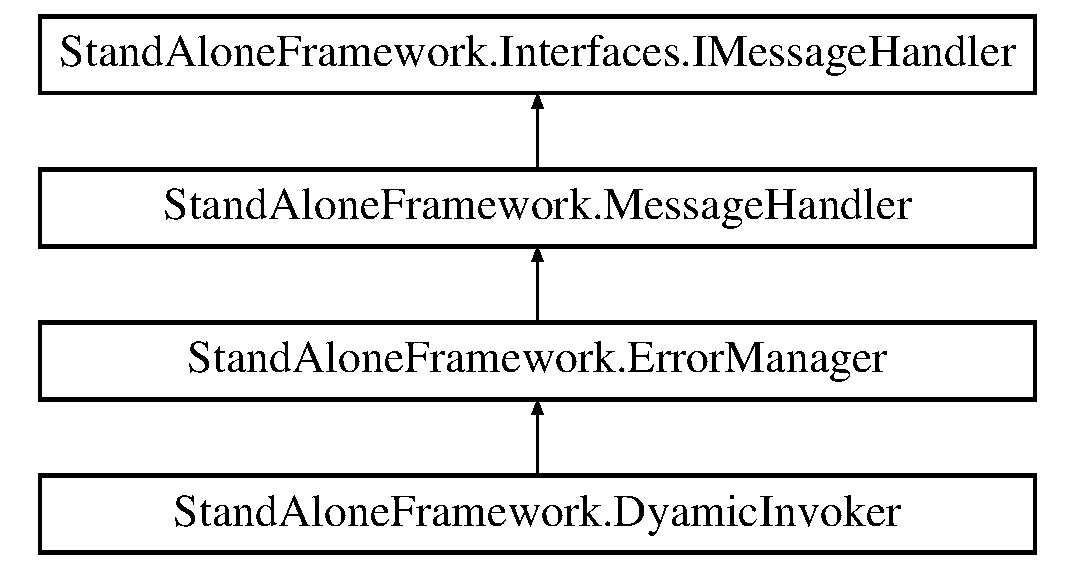
\includegraphics[height=4.000000cm]{class_stand_alone_framework_1_1_message_handler}
\end{center}
\end{figure}
\subsection*{Public Member Functions}
\begin{DoxyCompactItemize}
\item 
void \hyperlink{class_stand_alone_framework_1_1_message_handler_af3c85f52f95dcfb2d10edc8238cf885e}{Show\+Message} (\hyperlink{class_stand_alone_framework_1_1_framework_classes_1_1_invocation_result}{Invocation\+Result} invocation\+Result)
\begin{DoxyCompactList}\small\item\em Shows the message to a particular consumer -\/ could be a separate message bus or a simple front end such as a Console. \end{DoxyCompactList}\end{DoxyCompactItemize}


\subsection{Detailed Description}
Acts as a central message handler. This would defer all the message displaying functionality to either the front end, or could be used together M\+S\+M\+Q 



\subsection{Member Function Documentation}
\hypertarget{class_stand_alone_framework_1_1_message_handler_af3c85f52f95dcfb2d10edc8238cf885e}{\index{Stand\+Alone\+Framework\+::\+Message\+Handler@{Stand\+Alone\+Framework\+::\+Message\+Handler}!Show\+Message@{Show\+Message}}
\index{Show\+Message@{Show\+Message}!Stand\+Alone\+Framework\+::\+Message\+Handler@{Stand\+Alone\+Framework\+::\+Message\+Handler}}
\subsubsection[{Show\+Message}]{\setlength{\rightskip}{0pt plus 5cm}void Stand\+Alone\+Framework.\+Message\+Handler.\+Show\+Message (
\begin{DoxyParamCaption}
\item[{{\bf Invocation\+Result}}]{invocation\+Result}
\end{DoxyParamCaption}
)}}\label{class_stand_alone_framework_1_1_message_handler_af3c85f52f95dcfb2d10edc8238cf885e}


Shows the message to a particular consumer -\/ could be a separate message bus or a simple front end such as a Console. 


\begin{DoxyParams}{Parameters}
{\em invocation\+Result} & The invocation result.\\
\hline
\end{DoxyParams}


The documentation for this class was generated from the following file\+:\begin{DoxyCompactItemize}
\item 
C\+:/\+Users/\+Charles Trent Spare/\+Documents/\+Source Control/\+Repositories/\+Development\+Projects/\+Stand\+Alone\+Framework/\+Stand\+Alone\+Framework/\+Message\+Handler/\hyperlink{_message_handler_8cs}{Message\+Handler.\+cs}\end{DoxyCompactItemize}

\hypertarget{class_stand_alone_framework_1_1_method_facade_1_1_method_facade}{\section{Stand\+Alone\+Framework.\+Method\+Facade.\+Method\+Facade Class Reference}
\label{class_stand_alone_framework_1_1_method_facade_1_1_method_facade}\index{Stand\+Alone\+Framework.\+Method\+Facade.\+Method\+Facade@{Stand\+Alone\+Framework.\+Method\+Facade.\+Method\+Facade}}
}


Represents the facade or entry point of all method calls into the framework  


Inheritance diagram for Stand\+Alone\+Framework.\+Method\+Facade.\+Method\+Facade\+:\begin{figure}[H]
\begin{center}
\leavevmode
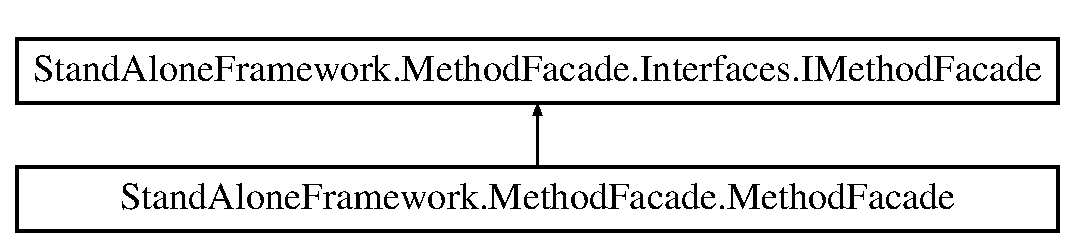
\includegraphics[height=2.000000cm]{class_stand_alone_framework_1_1_method_facade_1_1_method_facade}
\end{center}
\end{figure}
\subsection*{Public Member Functions}
\begin{DoxyCompactItemize}
\item 
\hyperlink{class_stand_alone_framework_1_1_method_facade_1_1_method_facade_a8b2622fdb38b2a9f1bab372ef196b05d}{Method\+Facade} ()
\begin{DoxyCompactList}\small\item\em Initializes a new instance of the \hyperlink{class_stand_alone_framework_1_1_method_facade_1_1_method_facade}{Method\+Facade} class. \end{DoxyCompactList}\end{DoxyCompactItemize}
\subsection*{Properties}
\begin{DoxyCompactItemize}
\item 
\hyperlink{interface_stand_alone_framework_1_1_factories_1_1_interfaces_1_1_i_method_factory}{I\+Method\+Factory} \hyperlink{class_stand_alone_framework_1_1_method_facade_1_1_method_facade_ac9d757f293315f65a4d33668c81f05f4}{Method\+Factory}\hspace{0.3cm}{\ttfamily  \mbox{[}get, set\mbox{]}}
\begin{DoxyCompactList}\small\item\em Gets or sets the method factory. \end{DoxyCompactList}\end{DoxyCompactItemize}


\subsection{Detailed Description}
Represents the facade or entry point of all method calls into the framework 



\subsection{Constructor \& Destructor Documentation}
\hypertarget{class_stand_alone_framework_1_1_method_facade_1_1_method_facade_a8b2622fdb38b2a9f1bab372ef196b05d}{\index{Stand\+Alone\+Framework\+::\+Method\+Facade\+::\+Method\+Facade@{Stand\+Alone\+Framework\+::\+Method\+Facade\+::\+Method\+Facade}!Method\+Facade@{Method\+Facade}}
\index{Method\+Facade@{Method\+Facade}!Stand\+Alone\+Framework\+::\+Method\+Facade\+::\+Method\+Facade@{Stand\+Alone\+Framework\+::\+Method\+Facade\+::\+Method\+Facade}}
\subsubsection[{Method\+Facade}]{\setlength{\rightskip}{0pt plus 5cm}Stand\+Alone\+Framework.\+Method\+Facade.\+Method\+Facade.\+Method\+Facade (
\begin{DoxyParamCaption}
{}
\end{DoxyParamCaption}
)}}\label{class_stand_alone_framework_1_1_method_facade_1_1_method_facade_a8b2622fdb38b2a9f1bab372ef196b05d}


Initializes a new instance of the \hyperlink{class_stand_alone_framework_1_1_method_facade_1_1_method_facade}{Method\+Facade} class. 



\subsection{Property Documentation}
\hypertarget{class_stand_alone_framework_1_1_method_facade_1_1_method_facade_ac9d757f293315f65a4d33668c81f05f4}{\index{Stand\+Alone\+Framework\+::\+Method\+Facade\+::\+Method\+Facade@{Stand\+Alone\+Framework\+::\+Method\+Facade\+::\+Method\+Facade}!Method\+Factory@{Method\+Factory}}
\index{Method\+Factory@{Method\+Factory}!Stand\+Alone\+Framework\+::\+Method\+Facade\+::\+Method\+Facade@{Stand\+Alone\+Framework\+::\+Method\+Facade\+::\+Method\+Facade}}
\subsubsection[{Method\+Factory}]{\setlength{\rightskip}{0pt plus 5cm}{\bf I\+Method\+Factory} Stand\+Alone\+Framework.\+Method\+Facade.\+Method\+Facade.\+Method\+Factory\hspace{0.3cm}{\ttfamily [get]}, {\ttfamily [set]}}}\label{class_stand_alone_framework_1_1_method_facade_1_1_method_facade_ac9d757f293315f65a4d33668c81f05f4}


Gets or sets the method factory. 

The method factory.

The documentation for this class was generated from the following file\+:\begin{DoxyCompactItemize}
\item 
C\+:/\+Users/\+Charles Trent Spare/\+Documents/\+Source Control/\+Repositories/\+Development\+Projects/\+Stand\+Alone\+Framework/\+Stand\+Alone\+Framework/\+Method\+Facade/\hyperlink{_method_facade_8cs}{Method\+Facade.\+cs}\end{DoxyCompactItemize}

\hypertarget{class_stand_alone_framework_1_1_factories_1_1_method_factory_1_1_method_factory}{\section{Stand\+Alone\+Framework.\+Factories.\+Method\+Factory.\+Method\+Factory Class Reference}
\label{class_stand_alone_framework_1_1_factories_1_1_method_factory_1_1_method_factory}\index{Stand\+Alone\+Framework.\+Factories.\+Method\+Factory.\+Method\+Factory@{Stand\+Alone\+Framework.\+Factories.\+Method\+Factory.\+Method\+Factory}}
}


Encapsulates functionality that creates and wraps a method with a thread as well as any arguments that the method requires.  


Inheritance diagram for Stand\+Alone\+Framework.\+Factories.\+Method\+Factory.\+Method\+Factory\+:\begin{figure}[H]
\begin{center}
\leavevmode
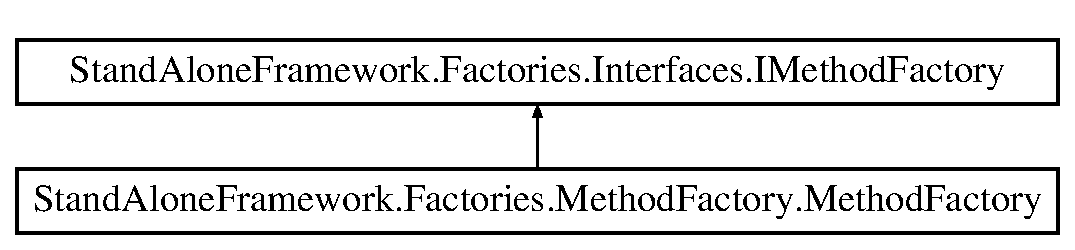
\includegraphics[height=2.000000cm]{class_stand_alone_framework_1_1_factories_1_1_method_factory_1_1_method_factory}
\end{center}
\end{figure}
\subsection*{Public Member Functions}
\begin{DoxyCompactItemize}
\item 
\hyperlink{class_stand_alone_framework_1_1_factories_1_1_method_factory_1_1_method_factory_a03c9d9ba7c468c89fd8e0e791033fa5d}{Method\+Factory} ()
\begin{DoxyCompactList}\small\item\em Initializes a new instance of the \hyperlink{class_stand_alone_framework_1_1_factories_1_1_method_factory_1_1_method_factory}{Method\+Factory} class. \end{DoxyCompactList}\item 
object \hyperlink{class_stand_alone_framework_1_1_factories_1_1_method_factory_1_1_method_factory_a5e1c85f6928f23809770682565ce18ef}{Execute\+Method} ()
\begin{DoxyCompactList}\small\item\em Executes the method. \end{DoxyCompactList}\item 
void \hyperlink{class_stand_alone_framework_1_1_factories_1_1_method_factory_1_1_method_factory_ad7266b9459d17e8931b267470a3f65a3}{Start\+Factory} (\hyperlink{namespace_stand_alone_framework_1_1_factories_1_1_method_factory_a03ffbf0d8e733b86d0ac29ae38dd4241}{Method\+Return\+Type} method\+Return\+Type, \hyperlink{namespace_stand_alone_framework_1_1_factories_1_1_method_factory_aeb6e05dc016e73b072faae5a5d275f6a}{Method\+Type} method\+Type, \hyperlink{namespace_stand_alone_framework_1_1_factories_1_1_thread_factory_aaa02326f96ee10b7d0fd360488d27c39}{Threading\+Model} threading\+Model, object method\+To\+Invoke, \hyperlink{class_stand_alone_framework_1_1_data_wrapper}{Data\+Wrapper} args)
\begin{DoxyCompactList}\small\item\em Starts the factory. \end{DoxyCompactList}\end{DoxyCompactItemize}
\subsection*{Properties}
\begin{DoxyCompactItemize}
\item 
\hyperlink{interface_stand_alone_framework_1_1_factories_1_1_interfaces_1_1_i_thread_factory}{I\+Thread\+Factory} \hyperlink{class_stand_alone_framework_1_1_factories_1_1_method_factory_1_1_method_factory_a42dbb8efe86a1f9724b65097bcef9efd}{Thread\+Factory}\hspace{0.3cm}{\ttfamily  \mbox{[}get, set\mbox{]}}
\begin{DoxyCompactList}\small\item\em Gets or sets the thread factory. \end{DoxyCompactList}\item 
\hyperlink{class_stand_alone_framework_1_1_factories_1_1_method_factory_1_1_method_wrapper}{Method\+Wrapper} \hyperlink{class_stand_alone_framework_1_1_factories_1_1_method_factory_1_1_method_factory_a1be5b47ac05d4e1fb9fbf29cc185019e}{Method\+Wrapper}\hspace{0.3cm}{\ttfamily  \mbox{[}get, set\mbox{]}}
\begin{DoxyCompactList}\small\item\em Gets or sets the method wrapper. \end{DoxyCompactList}\end{DoxyCompactItemize}


\subsection{Detailed Description}
Encapsulates functionality that creates and wraps a method with a thread as well as any arguments that the method requires. 



\subsection{Constructor \& Destructor Documentation}
\hypertarget{class_stand_alone_framework_1_1_factories_1_1_method_factory_1_1_method_factory_a03c9d9ba7c468c89fd8e0e791033fa5d}{\index{Stand\+Alone\+Framework\+::\+Factories\+::\+Method\+Factory\+::\+Method\+Factory@{Stand\+Alone\+Framework\+::\+Factories\+::\+Method\+Factory\+::\+Method\+Factory}!Method\+Factory@{Method\+Factory}}
\index{Method\+Factory@{Method\+Factory}!Stand\+Alone\+Framework\+::\+Factories\+::\+Method\+Factory\+::\+Method\+Factory@{Stand\+Alone\+Framework\+::\+Factories\+::\+Method\+Factory\+::\+Method\+Factory}}
\subsubsection[{Method\+Factory}]{\setlength{\rightskip}{0pt plus 5cm}Stand\+Alone\+Framework.\+Factories.\+Method\+Factory.\+Method\+Factory.\+Method\+Factory (
\begin{DoxyParamCaption}
{}
\end{DoxyParamCaption}
)}}\label{class_stand_alone_framework_1_1_factories_1_1_method_factory_1_1_method_factory_a03c9d9ba7c468c89fd8e0e791033fa5d}


Initializes a new instance of the \hyperlink{class_stand_alone_framework_1_1_factories_1_1_method_factory_1_1_method_factory}{Method\+Factory} class. 



\subsection{Member Function Documentation}
\hypertarget{class_stand_alone_framework_1_1_factories_1_1_method_factory_1_1_method_factory_a5e1c85f6928f23809770682565ce18ef}{\index{Stand\+Alone\+Framework\+::\+Factories\+::\+Method\+Factory\+::\+Method\+Factory@{Stand\+Alone\+Framework\+::\+Factories\+::\+Method\+Factory\+::\+Method\+Factory}!Execute\+Method@{Execute\+Method}}
\index{Execute\+Method@{Execute\+Method}!Stand\+Alone\+Framework\+::\+Factories\+::\+Method\+Factory\+::\+Method\+Factory@{Stand\+Alone\+Framework\+::\+Factories\+::\+Method\+Factory\+::\+Method\+Factory}}
\subsubsection[{Execute\+Method}]{\setlength{\rightskip}{0pt plus 5cm}object Stand\+Alone\+Framework.\+Factories.\+Method\+Factory.\+Method\+Factory.\+Execute\+Method (
\begin{DoxyParamCaption}
{}
\end{DoxyParamCaption}
)}}\label{class_stand_alone_framework_1_1_factories_1_1_method_factory_1_1_method_factory_a5e1c85f6928f23809770682565ce18ef}


Executes the method. 

\begin{DoxyReturn}{Returns}
An instance of type Invocation\+Result
\end{DoxyReturn}


Implements \hyperlink{interface_stand_alone_framework_1_1_factories_1_1_interfaces_1_1_i_method_factory_a699e7a06cdb746034ce0d7b38d9cf21c}{Stand\+Alone\+Framework.\+Factories.\+Interfaces.\+I\+Method\+Factory}.

\hypertarget{class_stand_alone_framework_1_1_factories_1_1_method_factory_1_1_method_factory_ad7266b9459d17e8931b267470a3f65a3}{\index{Stand\+Alone\+Framework\+::\+Factories\+::\+Method\+Factory\+::\+Method\+Factory@{Stand\+Alone\+Framework\+::\+Factories\+::\+Method\+Factory\+::\+Method\+Factory}!Start\+Factory@{Start\+Factory}}
\index{Start\+Factory@{Start\+Factory}!Stand\+Alone\+Framework\+::\+Factories\+::\+Method\+Factory\+::\+Method\+Factory@{Stand\+Alone\+Framework\+::\+Factories\+::\+Method\+Factory\+::\+Method\+Factory}}
\subsubsection[{Start\+Factory}]{\setlength{\rightskip}{0pt plus 5cm}void Stand\+Alone\+Framework.\+Factories.\+Method\+Factory.\+Method\+Factory.\+Start\+Factory (
\begin{DoxyParamCaption}
\item[{{\bf Method\+Return\+Type}}]{method\+Return\+Type, }
\item[{{\bf Method\+Type}}]{method\+Type, }
\item[{{\bf Threading\+Model}}]{threading\+Model, }
\item[{object}]{method\+To\+Invoke, }
\item[{{\bf Data\+Wrapper}}]{args}
\end{DoxyParamCaption}
)}}\label{class_stand_alone_framework_1_1_factories_1_1_method_factory_1_1_method_factory_ad7266b9459d17e8931b267470a3f65a3}


Starts the factory. 


\begin{DoxyParams}{Parameters}
{\em method\+Return\+Type} & The method return type.\\
\hline
{\em method\+Type} & Type of the method.\\
\hline
{\em threading\+Model} & The threading model to use during runtime.\\
\hline
{\em method\+To\+Invoke} & The method to invoke.\\
\hline
{\em args} & The arguments for the method\\
\hline
\end{DoxyParams}


Implements \hyperlink{interface_stand_alone_framework_1_1_factories_1_1_interfaces_1_1_i_method_factory_aafd802da0b25eaf9e11c53b9c0d06bdf}{Stand\+Alone\+Framework.\+Factories.\+Interfaces.\+I\+Method\+Factory}.



\subsection{Property Documentation}
\hypertarget{class_stand_alone_framework_1_1_factories_1_1_method_factory_1_1_method_factory_a1be5b47ac05d4e1fb9fbf29cc185019e}{\index{Stand\+Alone\+Framework\+::\+Factories\+::\+Method\+Factory\+::\+Method\+Factory@{Stand\+Alone\+Framework\+::\+Factories\+::\+Method\+Factory\+::\+Method\+Factory}!Method\+Wrapper@{Method\+Wrapper}}
\index{Method\+Wrapper@{Method\+Wrapper}!Stand\+Alone\+Framework\+::\+Factories\+::\+Method\+Factory\+::\+Method\+Factory@{Stand\+Alone\+Framework\+::\+Factories\+::\+Method\+Factory\+::\+Method\+Factory}}
\subsubsection[{Method\+Wrapper}]{\setlength{\rightskip}{0pt plus 5cm}{\bf Method\+Wrapper} Stand\+Alone\+Framework.\+Factories.\+Method\+Factory.\+Method\+Factory.\+Method\+Wrapper\hspace{0.3cm}{\ttfamily [get]}, {\ttfamily [set]}}}\label{class_stand_alone_framework_1_1_factories_1_1_method_factory_1_1_method_factory_a1be5b47ac05d4e1fb9fbf29cc185019e}


Gets or sets the method wrapper. 

The method wrapper.\hypertarget{class_stand_alone_framework_1_1_factories_1_1_method_factory_1_1_method_factory_a42dbb8efe86a1f9724b65097bcef9efd}{\index{Stand\+Alone\+Framework\+::\+Factories\+::\+Method\+Factory\+::\+Method\+Factory@{Stand\+Alone\+Framework\+::\+Factories\+::\+Method\+Factory\+::\+Method\+Factory}!Thread\+Factory@{Thread\+Factory}}
\index{Thread\+Factory@{Thread\+Factory}!Stand\+Alone\+Framework\+::\+Factories\+::\+Method\+Factory\+::\+Method\+Factory@{Stand\+Alone\+Framework\+::\+Factories\+::\+Method\+Factory\+::\+Method\+Factory}}
\subsubsection[{Thread\+Factory}]{\setlength{\rightskip}{0pt plus 5cm}{\bf I\+Thread\+Factory} Stand\+Alone\+Framework.\+Factories.\+Method\+Factory.\+Method\+Factory.\+Thread\+Factory\hspace{0.3cm}{\ttfamily [get]}, {\ttfamily [set]}}}\label{class_stand_alone_framework_1_1_factories_1_1_method_factory_1_1_method_factory_a42dbb8efe86a1f9724b65097bcef9efd}


Gets or sets the thread factory. 

The thread factory.

The documentation for this class was generated from the following file\+:\begin{DoxyCompactItemize}
\item 
C\+:/\+Users/\+Charles Trent Spare/\+Documents/\+Source Control/\+Repositories/\+Development\+Projects/\+Stand\+Alone\+Framework/\+Stand\+Alone\+Framework/\+Factories/\+Method\+Factory/\hyperlink{_method_factory_8cs}{Method\+Factory.\+cs}\end{DoxyCompactItemize}

\hypertarget{class_stand_alone_framework_1_1_factories_1_1_method_factory_1_1_method_wrapper}{\section{Stand\+Alone\+Framework.\+Factories.\+Method\+Factory.\+Method\+Wrapper Class Reference}
\label{class_stand_alone_framework_1_1_factories_1_1_method_factory_1_1_method_wrapper}\index{Stand\+Alone\+Framework.\+Factories.\+Method\+Factory.\+Method\+Wrapper@{Stand\+Alone\+Framework.\+Factories.\+Method\+Factory.\+Method\+Wrapper}}
}


Class \hyperlink{class_stand_alone_framework_1_1_factories_1_1_method_factory_1_1_method_wrapper}{Method\+Wrapper}  


\subsection*{Properties}
\begin{DoxyCompactItemize}
\item 
\hyperlink{namespace_stand_alone_framework_1_1_factories_1_1_method_factory_a03ffbf0d8e733b86d0ac29ae38dd4241}{Method\+Return\+Type} \hyperlink{class_stand_alone_framework_1_1_factories_1_1_method_factory_1_1_method_wrapper_a51c9c1a1bcf1d278aaed5eecb4d12ca1}{Method\+Return\+Type}\hspace{0.3cm}{\ttfamily  \mbox{[}get, set\mbox{]}}
\begin{DoxyCompactList}\small\item\em Gets or sets the method return type. \end{DoxyCompactList}\item 
\hyperlink{namespace_stand_alone_framework_1_1_factories_1_1_method_factory_aeb6e05dc016e73b072faae5a5d275f6a}{Method\+Type} \hyperlink{class_stand_alone_framework_1_1_factories_1_1_method_factory_1_1_method_wrapper_a5f43e091e43ccf5bf9744aa24da0fe43}{Method\+Type}\hspace{0.3cm}{\ttfamily  \mbox{[}get, set\mbox{]}}
\begin{DoxyCompactList}\small\item\em Gets or sets the method type \end{DoxyCompactList}\item 
\hyperlink{namespace_stand_alone_framework_1_1_factories_1_1_thread_factory_aaa02326f96ee10b7d0fd360488d27c39}{Threading\+Model} \hyperlink{class_stand_alone_framework_1_1_factories_1_1_method_factory_1_1_method_wrapper_ad81cf5c2f772eea08b0f64ea0032d44b}{Threading\+Model}\hspace{0.3cm}{\ttfamily  \mbox{[}get, set\mbox{]}}
\begin{DoxyCompactList}\small\item\em Gets or sets the type of threading to use during execution. \end{DoxyCompactList}\item 
\hyperlink{class_stand_alone_framework_1_1_data_wrapper}{Data\+Wrapper} \hyperlink{class_stand_alone_framework_1_1_factories_1_1_method_factory_1_1_method_wrapper_ab9972e5f2931cf4af0fbf5571a97db6a}{Arguments}\hspace{0.3cm}{\ttfamily  \mbox{[}get, set\mbox{]}}
\begin{DoxyCompactList}\small\item\em Gets or sets the arguments that are passed into the method. \end{DoxyCompactList}\item 
Thread \hyperlink{class_stand_alone_framework_1_1_factories_1_1_method_factory_1_1_method_wrapper_a53705992cdbe995cf7099e806ff2b51c}{Executing\+Thread}\hspace{0.3cm}{\ttfamily  \mbox{[}get, set\mbox{]}}
\begin{DoxyCompactList}\small\item\em Gets or sets the executing thread that acts as the container for the method. \end{DoxyCompactList}\item 
\hyperlink{namespace_stand_alone_framework_1_1_factories_1_1_method_factory_aeb6e05dc016e73b072faae5a5d275f6aa004bf6c9a40003140292e97330236c53}{Action}$<$ \hyperlink{class_stand_alone_framework_1_1_data_wrapper}{Data\+Wrapper} $>$ \hyperlink{class_stand_alone_framework_1_1_factories_1_1_method_factory_1_1_method_wrapper_ab783cacf95f59ff0df1f3b36d981c468}{Action\+Method}\hspace{0.3cm}{\ttfamily  \mbox{[}get, set\mbox{]}}
\begin{DoxyCompactList}\small\item\em Gets or sets the action method. \end{DoxyCompactList}\item 
\hyperlink{namespace_stand_alone_framework_1_1_factories_1_1_method_factory_aeb6e05dc016e73b072faae5a5d275f6aa00d0b4f2d7dcdaaef835b97cf5d1e0df}{Func}$<$ \hyperlink{class_stand_alone_framework_1_1_data_wrapper}{Data\+Wrapper}, \\*
\hyperlink{class_stand_alone_framework_1_1_framework_classes_1_1_invocation_result}{Invocation\+Result} $>$ \hyperlink{class_stand_alone_framework_1_1_factories_1_1_method_factory_1_1_method_wrapper_a3a7ae8b79a922646649ffea70f5e60e9}{Func\+Method}\hspace{0.3cm}{\ttfamily  \mbox{[}get, set\mbox{]}}
\begin{DoxyCompactList}\small\item\em Gets or sets the function method. \end{DoxyCompactList}\end{DoxyCompactItemize}


\subsection{Detailed Description}
Class \hyperlink{class_stand_alone_framework_1_1_factories_1_1_method_factory_1_1_method_wrapper}{Method\+Wrapper} 



\subsection{Property Documentation}
\hypertarget{class_stand_alone_framework_1_1_factories_1_1_method_factory_1_1_method_wrapper_ab783cacf95f59ff0df1f3b36d981c468}{\index{Stand\+Alone\+Framework\+::\+Factories\+::\+Method\+Factory\+::\+Method\+Wrapper@{Stand\+Alone\+Framework\+::\+Factories\+::\+Method\+Factory\+::\+Method\+Wrapper}!Action\+Method@{Action\+Method}}
\index{Action\+Method@{Action\+Method}!Stand\+Alone\+Framework\+::\+Factories\+::\+Method\+Factory\+::\+Method\+Wrapper@{Stand\+Alone\+Framework\+::\+Factories\+::\+Method\+Factory\+::\+Method\+Wrapper}}
\subsubsection[{Action\+Method}]{\setlength{\rightskip}{0pt plus 5cm}{\bf Action}$<${\bf Data\+Wrapper}$>$ Stand\+Alone\+Framework.\+Factories.\+Method\+Factory.\+Method\+Wrapper.\+Action\+Method\hspace{0.3cm}{\ttfamily [get]}, {\ttfamily [set]}}}\label{class_stand_alone_framework_1_1_factories_1_1_method_factory_1_1_method_wrapper_ab783cacf95f59ff0df1f3b36d981c468}


Gets or sets the action method. 

The action method.\hypertarget{class_stand_alone_framework_1_1_factories_1_1_method_factory_1_1_method_wrapper_ab9972e5f2931cf4af0fbf5571a97db6a}{\index{Stand\+Alone\+Framework\+::\+Factories\+::\+Method\+Factory\+::\+Method\+Wrapper@{Stand\+Alone\+Framework\+::\+Factories\+::\+Method\+Factory\+::\+Method\+Wrapper}!Arguments@{Arguments}}
\index{Arguments@{Arguments}!Stand\+Alone\+Framework\+::\+Factories\+::\+Method\+Factory\+::\+Method\+Wrapper@{Stand\+Alone\+Framework\+::\+Factories\+::\+Method\+Factory\+::\+Method\+Wrapper}}
\subsubsection[{Arguments}]{\setlength{\rightskip}{0pt plus 5cm}{\bf Data\+Wrapper} Stand\+Alone\+Framework.\+Factories.\+Method\+Factory.\+Method\+Wrapper.\+Arguments\hspace{0.3cm}{\ttfamily [get]}, {\ttfamily [set]}}}\label{class_stand_alone_framework_1_1_factories_1_1_method_factory_1_1_method_wrapper_ab9972e5f2931cf4af0fbf5571a97db6a}


Gets or sets the arguments that are passed into the method. 

The arguments.\hypertarget{class_stand_alone_framework_1_1_factories_1_1_method_factory_1_1_method_wrapper_a53705992cdbe995cf7099e806ff2b51c}{\index{Stand\+Alone\+Framework\+::\+Factories\+::\+Method\+Factory\+::\+Method\+Wrapper@{Stand\+Alone\+Framework\+::\+Factories\+::\+Method\+Factory\+::\+Method\+Wrapper}!Executing\+Thread@{Executing\+Thread}}
\index{Executing\+Thread@{Executing\+Thread}!Stand\+Alone\+Framework\+::\+Factories\+::\+Method\+Factory\+::\+Method\+Wrapper@{Stand\+Alone\+Framework\+::\+Factories\+::\+Method\+Factory\+::\+Method\+Wrapper}}
\subsubsection[{Executing\+Thread}]{\setlength{\rightskip}{0pt plus 5cm}Thread Stand\+Alone\+Framework.\+Factories.\+Method\+Factory.\+Method\+Wrapper.\+Executing\+Thread\hspace{0.3cm}{\ttfamily [get]}, {\ttfamily [set]}}}\label{class_stand_alone_framework_1_1_factories_1_1_method_factory_1_1_method_wrapper_a53705992cdbe995cf7099e806ff2b51c}


Gets or sets the executing thread that acts as the container for the method. 

The executing thread.\hypertarget{class_stand_alone_framework_1_1_factories_1_1_method_factory_1_1_method_wrapper_a3a7ae8b79a922646649ffea70f5e60e9}{\index{Stand\+Alone\+Framework\+::\+Factories\+::\+Method\+Factory\+::\+Method\+Wrapper@{Stand\+Alone\+Framework\+::\+Factories\+::\+Method\+Factory\+::\+Method\+Wrapper}!Func\+Method@{Func\+Method}}
\index{Func\+Method@{Func\+Method}!Stand\+Alone\+Framework\+::\+Factories\+::\+Method\+Factory\+::\+Method\+Wrapper@{Stand\+Alone\+Framework\+::\+Factories\+::\+Method\+Factory\+::\+Method\+Wrapper}}
\subsubsection[{Func\+Method}]{\setlength{\rightskip}{0pt plus 5cm}{\bf Func}$<${\bf Data\+Wrapper}, {\bf Invocation\+Result}$>$ Stand\+Alone\+Framework.\+Factories.\+Method\+Factory.\+Method\+Wrapper.\+Func\+Method\hspace{0.3cm}{\ttfamily [get]}, {\ttfamily [set]}}}\label{class_stand_alone_framework_1_1_factories_1_1_method_factory_1_1_method_wrapper_a3a7ae8b79a922646649ffea70f5e60e9}


Gets or sets the function method. 

The function method.\hypertarget{class_stand_alone_framework_1_1_factories_1_1_method_factory_1_1_method_wrapper_a51c9c1a1bcf1d278aaed5eecb4d12ca1}{\index{Stand\+Alone\+Framework\+::\+Factories\+::\+Method\+Factory\+::\+Method\+Wrapper@{Stand\+Alone\+Framework\+::\+Factories\+::\+Method\+Factory\+::\+Method\+Wrapper}!Method\+Return\+Type@{Method\+Return\+Type}}
\index{Method\+Return\+Type@{Method\+Return\+Type}!Stand\+Alone\+Framework\+::\+Factories\+::\+Method\+Factory\+::\+Method\+Wrapper@{Stand\+Alone\+Framework\+::\+Factories\+::\+Method\+Factory\+::\+Method\+Wrapper}}
\subsubsection[{Method\+Return\+Type}]{\setlength{\rightskip}{0pt plus 5cm}{\bf Method\+Return\+Type} Stand\+Alone\+Framework.\+Factories.\+Method\+Factory.\+Method\+Wrapper.\+Method\+Return\+Type\hspace{0.3cm}{\ttfamily [get]}, {\ttfamily [set]}}}\label{class_stand_alone_framework_1_1_factories_1_1_method_factory_1_1_method_wrapper_a51c9c1a1bcf1d278aaed5eecb4d12ca1}


Gets or sets the method return type. 

The type of the method return.\hypertarget{class_stand_alone_framework_1_1_factories_1_1_method_factory_1_1_method_wrapper_a5f43e091e43ccf5bf9744aa24da0fe43}{\index{Stand\+Alone\+Framework\+::\+Factories\+::\+Method\+Factory\+::\+Method\+Wrapper@{Stand\+Alone\+Framework\+::\+Factories\+::\+Method\+Factory\+::\+Method\+Wrapper}!Method\+Type@{Method\+Type}}
\index{Method\+Type@{Method\+Type}!Stand\+Alone\+Framework\+::\+Factories\+::\+Method\+Factory\+::\+Method\+Wrapper@{Stand\+Alone\+Framework\+::\+Factories\+::\+Method\+Factory\+::\+Method\+Wrapper}}
\subsubsection[{Method\+Type}]{\setlength{\rightskip}{0pt plus 5cm}{\bf Method\+Type} Stand\+Alone\+Framework.\+Factories.\+Method\+Factory.\+Method\+Wrapper.\+Method\+Type\hspace{0.3cm}{\ttfamily [get]}, {\ttfamily [set]}}}\label{class_stand_alone_framework_1_1_factories_1_1_method_factory_1_1_method_wrapper_a5f43e091e43ccf5bf9744aa24da0fe43}


Gets or sets the method type 

The type of the method.\hypertarget{class_stand_alone_framework_1_1_factories_1_1_method_factory_1_1_method_wrapper_ad81cf5c2f772eea08b0f64ea0032d44b}{\index{Stand\+Alone\+Framework\+::\+Factories\+::\+Method\+Factory\+::\+Method\+Wrapper@{Stand\+Alone\+Framework\+::\+Factories\+::\+Method\+Factory\+::\+Method\+Wrapper}!Threading\+Model@{Threading\+Model}}
\index{Threading\+Model@{Threading\+Model}!Stand\+Alone\+Framework\+::\+Factories\+::\+Method\+Factory\+::\+Method\+Wrapper@{Stand\+Alone\+Framework\+::\+Factories\+::\+Method\+Factory\+::\+Method\+Wrapper}}
\subsubsection[{Threading\+Model}]{\setlength{\rightskip}{0pt plus 5cm}{\bf Threading\+Model} Stand\+Alone\+Framework.\+Factories.\+Method\+Factory.\+Method\+Wrapper.\+Threading\+Model\hspace{0.3cm}{\ttfamily [get]}, {\ttfamily [set]}}}\label{class_stand_alone_framework_1_1_factories_1_1_method_factory_1_1_method_wrapper_ad81cf5c2f772eea08b0f64ea0032d44b}


Gets or sets the type of threading to use during execution. 

The threading model.

The documentation for this class was generated from the following file\+:\begin{DoxyCompactItemize}
\item 
C\+:/\+Users/\+Charles Trent Spare/\+Documents/\+Source Control/\+Repositories/\+Development\+Projects/\+Stand\+Alone\+Framework/\+Stand\+Alone\+Framework/\+Factories/\+Method\+Factory/\hyperlink{_method_factory_8cs}{Method\+Factory.\+cs}\end{DoxyCompactItemize}

\hypertarget{class_stand_alone_framework_test_1_1_stateful_tests_1_1_cache_manager_1_1_person}{\section{Stand\+Alone\+Framework\+Test.\+Stateful\+Tests.\+Cache\+Manager.\+Person Class Reference}
\label{class_stand_alone_framework_test_1_1_stateful_tests_1_1_cache_manager_1_1_person}\index{Stand\+Alone\+Framework\+Test.\+Stateful\+Tests.\+Cache\+Manager.\+Person@{Stand\+Alone\+Framework\+Test.\+Stateful\+Tests.\+Cache\+Manager.\+Person}}
}


The documentation for this class was generated from the following file\+:\begin{DoxyCompactItemize}
\item 
C\+:/\+Users/\+Charles Trent Spare/\+Documents/\+Source Control/\+Repositories/\+Development\+Projects/\+Stand\+Alone\+Framework/\+Stand\+Alone\+Framework/\+Stand\+Alone\+Framework\+Test/\+Stateful\+Tests/\+Cache\+Manager/\hyperlink{_cache_manger_test_fixture_8cs}{Cache\+Manger\+Test\+Fixture.\+cs}\end{DoxyCompactItemize}

\hypertarget{class_stand_alone_framework_1_1_factories_1_1_thread_factory_1_1_thread_factory}{\section{Stand\+Alone\+Framework.\+Factories.\+Thread\+Factory.\+Thread\+Factory Class Reference}
\label{class_stand_alone_framework_1_1_factories_1_1_thread_factory_1_1_thread_factory}\index{Stand\+Alone\+Framework.\+Factories.\+Thread\+Factory.\+Thread\+Factory@{Stand\+Alone\+Framework.\+Factories.\+Thread\+Factory.\+Thread\+Factory}}
}


Represents a factory that creates, terminates and handles any thread related tasks for the current method execution  


Inheritance diagram for Stand\+Alone\+Framework.\+Factories.\+Thread\+Factory.\+Thread\+Factory\+:\begin{figure}[H]
\begin{center}
\leavevmode
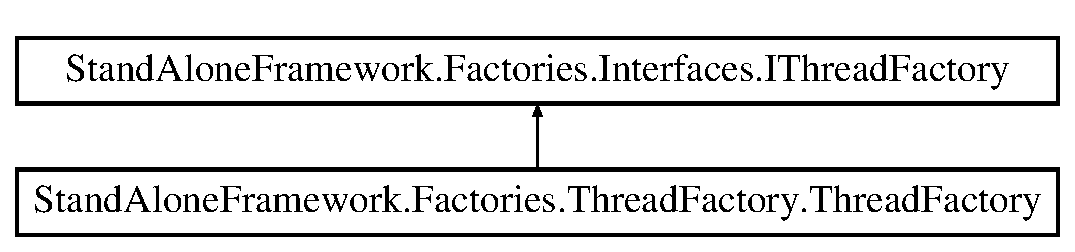
\includegraphics[height=2.000000cm]{class_stand_alone_framework_1_1_factories_1_1_thread_factory_1_1_thread_factory}
\end{center}
\end{figure}
\subsection*{Public Member Functions}
\begin{DoxyCompactItemize}
\item 
\hyperlink{class_stand_alone_framework_1_1_factories_1_1_thread_factory_1_1_thread_factory_a3720d6bf9aa95133f38ac3d9f01b1e1b}{Thread\+Factory} ()
\begin{DoxyCompactList}\small\item\em Initializes a new instance of the \hyperlink{class_stand_alone_framework_1_1_factories_1_1_thread_factory_1_1_thread_factory}{Thread\+Factory} class. \end{DoxyCompactList}\item 
void \hyperlink{class_stand_alone_framework_1_1_factories_1_1_thread_factory_1_1_thread_factory_a4fb8eb961ebeb6acfbaab63f169a1cb8}{Create\+Thread} (\hyperlink{class_stand_alone_framework_1_1_factories_1_1_method_factory_1_1_method_wrapper}{Method\+Wrapper} method\+Wrapper)
\begin{DoxyCompactList}\small\item\em Creates the thread. \end{DoxyCompactList}\item 
Thread \hyperlink{class_stand_alone_framework_1_1_factories_1_1_thread_factory_1_1_thread_factory_a19b01caebe842de7e8ac8989319af582}{Find\+Thread} (int thread\+Id)
\begin{DoxyCompactList}\small\item\em Finds the thread for the specific thread id. \end{DoxyCompactList}\end{DoxyCompactItemize}
\subsection*{Properties}
\begin{DoxyCompactItemize}
\item 
I\+List$<$ Thread $>$ \hyperlink{class_stand_alone_framework_1_1_factories_1_1_thread_factory_1_1_thread_factory_a47c41c0b106564ee96227cb93a276f4b}{Running\+Threads}\hspace{0.3cm}{\ttfamily  \mbox{[}get, set\mbox{]}}
\begin{DoxyCompactList}\small\item\em Gets or sets the running threads in the current method call. \end{DoxyCompactList}\end{DoxyCompactItemize}


\subsection{Detailed Description}
Represents a factory that creates, terminates and handles any thread related tasks for the current method execution 



\subsection{Constructor \& Destructor Documentation}
\hypertarget{class_stand_alone_framework_1_1_factories_1_1_thread_factory_1_1_thread_factory_a3720d6bf9aa95133f38ac3d9f01b1e1b}{\index{Stand\+Alone\+Framework\+::\+Factories\+::\+Thread\+Factory\+::\+Thread\+Factory@{Stand\+Alone\+Framework\+::\+Factories\+::\+Thread\+Factory\+::\+Thread\+Factory}!Thread\+Factory@{Thread\+Factory}}
\index{Thread\+Factory@{Thread\+Factory}!Stand\+Alone\+Framework\+::\+Factories\+::\+Thread\+Factory\+::\+Thread\+Factory@{Stand\+Alone\+Framework\+::\+Factories\+::\+Thread\+Factory\+::\+Thread\+Factory}}
\subsubsection[{Thread\+Factory}]{\setlength{\rightskip}{0pt plus 5cm}Stand\+Alone\+Framework.\+Factories.\+Thread\+Factory.\+Thread\+Factory.\+Thread\+Factory (
\begin{DoxyParamCaption}
{}
\end{DoxyParamCaption}
)}}\label{class_stand_alone_framework_1_1_factories_1_1_thread_factory_1_1_thread_factory_a3720d6bf9aa95133f38ac3d9f01b1e1b}


Initializes a new instance of the \hyperlink{class_stand_alone_framework_1_1_factories_1_1_thread_factory_1_1_thread_factory}{Thread\+Factory} class. 



\subsection{Member Function Documentation}
\hypertarget{class_stand_alone_framework_1_1_factories_1_1_thread_factory_1_1_thread_factory_a4fb8eb961ebeb6acfbaab63f169a1cb8}{\index{Stand\+Alone\+Framework\+::\+Factories\+::\+Thread\+Factory\+::\+Thread\+Factory@{Stand\+Alone\+Framework\+::\+Factories\+::\+Thread\+Factory\+::\+Thread\+Factory}!Create\+Thread@{Create\+Thread}}
\index{Create\+Thread@{Create\+Thread}!Stand\+Alone\+Framework\+::\+Factories\+::\+Thread\+Factory\+::\+Thread\+Factory@{Stand\+Alone\+Framework\+::\+Factories\+::\+Thread\+Factory\+::\+Thread\+Factory}}
\subsubsection[{Create\+Thread}]{\setlength{\rightskip}{0pt plus 5cm}void Stand\+Alone\+Framework.\+Factories.\+Thread\+Factory.\+Thread\+Factory.\+Create\+Thread (
\begin{DoxyParamCaption}
\item[{{\bf Method\+Wrapper}}]{method\+Wrapper}
\end{DoxyParamCaption}
)}}\label{class_stand_alone_framework_1_1_factories_1_1_thread_factory_1_1_thread_factory_a4fb8eb961ebeb6acfbaab63f169a1cb8}


Creates the thread. 


\begin{DoxyParams}{Parameters}
{\em method\+Wrapper} & The method wrapper.\\
\hline
\end{DoxyParams}


Implements \hyperlink{interface_stand_alone_framework_1_1_factories_1_1_interfaces_1_1_i_thread_factory_aa57ffdc6e7234b5377bfc4bdc319f985}{Stand\+Alone\+Framework.\+Factories.\+Interfaces.\+I\+Thread\+Factory}.

\hypertarget{class_stand_alone_framework_1_1_factories_1_1_thread_factory_1_1_thread_factory_a19b01caebe842de7e8ac8989319af582}{\index{Stand\+Alone\+Framework\+::\+Factories\+::\+Thread\+Factory\+::\+Thread\+Factory@{Stand\+Alone\+Framework\+::\+Factories\+::\+Thread\+Factory\+::\+Thread\+Factory}!Find\+Thread@{Find\+Thread}}
\index{Find\+Thread@{Find\+Thread}!Stand\+Alone\+Framework\+::\+Factories\+::\+Thread\+Factory\+::\+Thread\+Factory@{Stand\+Alone\+Framework\+::\+Factories\+::\+Thread\+Factory\+::\+Thread\+Factory}}
\subsubsection[{Find\+Thread}]{\setlength{\rightskip}{0pt plus 5cm}Thread Stand\+Alone\+Framework.\+Factories.\+Thread\+Factory.\+Thread\+Factory.\+Find\+Thread (
\begin{DoxyParamCaption}
\item[{int}]{thread\+Id}
\end{DoxyParamCaption}
)}}\label{class_stand_alone_framework_1_1_factories_1_1_thread_factory_1_1_thread_factory_a19b01caebe842de7e8ac8989319af582}


Finds the thread for the specific thread id. 


\begin{DoxyParams}{Parameters}
{\em thread\+Id} & The thread identifier.\\
\hline
\end{DoxyParams}
\begin{DoxyReturn}{Returns}
Thread.
\end{DoxyReturn}


Implements \hyperlink{interface_stand_alone_framework_1_1_factories_1_1_interfaces_1_1_i_thread_factory_a6a9c8007ba1e6738f7013089f1f9117c}{Stand\+Alone\+Framework.\+Factories.\+Interfaces.\+I\+Thread\+Factory}.



\subsection{Property Documentation}
\hypertarget{class_stand_alone_framework_1_1_factories_1_1_thread_factory_1_1_thread_factory_a47c41c0b106564ee96227cb93a276f4b}{\index{Stand\+Alone\+Framework\+::\+Factories\+::\+Thread\+Factory\+::\+Thread\+Factory@{Stand\+Alone\+Framework\+::\+Factories\+::\+Thread\+Factory\+::\+Thread\+Factory}!Running\+Threads@{Running\+Threads}}
\index{Running\+Threads@{Running\+Threads}!Stand\+Alone\+Framework\+::\+Factories\+::\+Thread\+Factory\+::\+Thread\+Factory@{Stand\+Alone\+Framework\+::\+Factories\+::\+Thread\+Factory\+::\+Thread\+Factory}}
\subsubsection[{Running\+Threads}]{\setlength{\rightskip}{0pt plus 5cm}I\+List$<$Thread$>$ Stand\+Alone\+Framework.\+Factories.\+Thread\+Factory.\+Thread\+Factory.\+Running\+Threads\hspace{0.3cm}{\ttfamily [get]}, {\ttfamily [set]}}}\label{class_stand_alone_framework_1_1_factories_1_1_thread_factory_1_1_thread_factory_a47c41c0b106564ee96227cb93a276f4b}


Gets or sets the running threads in the current method call. 

The running threads.

The documentation for this class was generated from the following file\+:\begin{DoxyCompactItemize}
\item 
C\+:/\+Users/\+Charles Trent Spare/\+Documents/\+Source Control/\+Repositories/\+Development\+Projects/\+Stand\+Alone\+Framework/\+Stand\+Alone\+Framework/\+Factories/\+Thread\+Factory/\hyperlink{_thread_factory_8cs}{Thread\+Factory.\+cs}\end{DoxyCompactItemize}

\chapter{File Documentation}
\hypertarget{_cache_manager_8cs}{\section{C\+:/\+Users/\+Charles Trent Spare/\+Documents/\+Source Control/\+Repositories/\+Development\+Projects/\+Stand\+Alone\+Framework/\+Stand\+Alone\+Framework/\+Cache\+Manager/\+Cache\+Manager.cs File Reference}
\label{_cache_manager_8cs}\index{C\+:/\+Users/\+Charles Trent Spare/\+Documents/\+Source Control/\+Repositories/\+Development\+Projects/\+Stand\+Alone\+Framework/\+Stand\+Alone\+Framework/\+Cache\+Manager/\+Cache\+Manager.\+cs@{C\+:/\+Users/\+Charles Trent Spare/\+Documents/\+Source Control/\+Repositories/\+Development\+Projects/\+Stand\+Alone\+Framework/\+Stand\+Alone\+Framework/\+Cache\+Manager/\+Cache\+Manager.\+cs}}
}
\subsection*{Classes}
\begin{DoxyCompactItemize}
\item 
class \hyperlink{class_stand_alone_framework_1_1_cache_manager_3_01_t_01_4}{Stand\+Alone\+Framework.\+Cache\+Manager$<$ T $>$}
\begin{DoxyCompactList}\small\item\em Acts as a central store for all objects who need to be cached \end{DoxyCompactList}\end{DoxyCompactItemize}
\subsection*{Namespaces}
\begin{DoxyCompactItemize}
\item 
package \hyperlink{namespace_stand_alone_framework}{Stand\+Alone\+Framework}
\end{DoxyCompactItemize}

\hypertarget{_i_cache_manager_8cs}{\section{C\+:/\+Users/\+Charles Trent Spare/\+Documents/\+Source Control/\+Repositories/\+Development\+Projects/\+Stand\+Alone\+Framework/\+Stand\+Alone\+Framework/\+Cache\+Manager/\+Interfaces/\+I\+Cache\+Manager.cs File Reference}
\label{_i_cache_manager_8cs}\index{C\+:/\+Users/\+Charles Trent Spare/\+Documents/\+Source Control/\+Repositories/\+Development\+Projects/\+Stand\+Alone\+Framework/\+Stand\+Alone\+Framework/\+Cache\+Manager/\+Interfaces/\+I\+Cache\+Manager.\+cs@{C\+:/\+Users/\+Charles Trent Spare/\+Documents/\+Source Control/\+Repositories/\+Development\+Projects/\+Stand\+Alone\+Framework/\+Stand\+Alone\+Framework/\+Cache\+Manager/\+Interfaces/\+I\+Cache\+Manager.\+cs}}
}
\subsection*{Classes}
\begin{DoxyCompactItemize}
\item 
interface \hyperlink{interface_stand_alone_framework_1_1_interfaces_1_1_i_cache_manager_3_01_t_01_4}{Stand\+Alone\+Framework.\+Interfaces.\+I\+Cache\+Manager$<$ T $>$}
\begin{DoxyCompactList}\small\item\em The Cache\+Manager's contract \end{DoxyCompactList}\end{DoxyCompactItemize}
\subsection*{Namespaces}
\begin{DoxyCompactItemize}
\item 
package \hyperlink{namespace_stand_alone_framework_1_1_interfaces}{Stand\+Alone\+Framework.\+Interfaces}
\end{DoxyCompactItemize}

\hypertarget{_code_contract_validator_8cs}{\section{C\+:/\+Users/\+Charles Trent Spare/\+Documents/\+Source Control/\+Repositories/\+Development\+Projects/\+Stand\+Alone\+Framework/\+Stand\+Alone\+Framework/\+Code\+Contract\+Validator/\+Code\+Contract\+Validator.cs File Reference}
\label{_code_contract_validator_8cs}\index{C\+:/\+Users/\+Charles Trent Spare/\+Documents/\+Source Control/\+Repositories/\+Development\+Projects/\+Stand\+Alone\+Framework/\+Stand\+Alone\+Framework/\+Code\+Contract\+Validator/\+Code\+Contract\+Validator.\+cs@{C\+:/\+Users/\+Charles Trent Spare/\+Documents/\+Source Control/\+Repositories/\+Development\+Projects/\+Stand\+Alone\+Framework/\+Stand\+Alone\+Framework/\+Code\+Contract\+Validator/\+Code\+Contract\+Validator.\+cs}}
}
\subsection*{Classes}
\begin{DoxyCompactItemize}
\item 
class \hyperlink{class_stand_alone_framework_1_1_code_contract_validator}{Stand\+Alone\+Framework.\+Code\+Contract\+Validator}
\begin{DoxyCompactList}\small\item\em Acts as a code contract validator. This is needed to ensure that all contracts conditions are met prior to any code execution \end{DoxyCompactList}\end{DoxyCompactItemize}
\subsection*{Namespaces}
\begin{DoxyCompactItemize}
\item 
package \hyperlink{namespace_stand_alone_framework}{Stand\+Alone\+Framework}
\end{DoxyCompactItemize}

\hypertarget{_data_wrapper_8cs}{\section{C\+:/\+Users/\+Charles Trent Spare/\+Documents/\+Source Control/\+Repositories/\+Development\+Projects/\+Stand\+Alone\+Framework/\+Stand\+Alone\+Framework/\+Data\+Wrapper.cs File Reference}
\label{_data_wrapper_8cs}\index{C\+:/\+Users/\+Charles Trent Spare/\+Documents/\+Source Control/\+Repositories/\+Development\+Projects/\+Stand\+Alone\+Framework/\+Stand\+Alone\+Framework/\+Data\+Wrapper.\+cs@{C\+:/\+Users/\+Charles Trent Spare/\+Documents/\+Source Control/\+Repositories/\+Development\+Projects/\+Stand\+Alone\+Framework/\+Stand\+Alone\+Framework/\+Data\+Wrapper.\+cs}}
}
\subsection*{Classes}
\begin{DoxyCompactItemize}
\item 
class \hyperlink{class_stand_alone_framework_1_1_data_wrapper}{Stand\+Alone\+Framework.\+Data\+Wrapper}
\begin{DoxyCompactList}\small\item\em Acts as a wrapper for the arguments that need to be passed into the method \end{DoxyCompactList}\end{DoxyCompactItemize}
\subsection*{Namespaces}
\begin{DoxyCompactItemize}
\item 
package \hyperlink{namespace_stand_alone_framework}{Stand\+Alone\+Framework}
\end{DoxyCompactItemize}

\hypertarget{_dyamic_invoker_8cs}{\section{C\+:/\+Users/\+Charles Trent Spare/\+Documents/\+Source Control/\+Repositories/\+Development\+Projects/\+Stand\+Alone\+Framework/\+Stand\+Alone\+Framework/\+Dynamic\+Invoker/\+Dyamic\+Invoker.cs File Reference}
\label{_dyamic_invoker_8cs}\index{C\+:/\+Users/\+Charles Trent Spare/\+Documents/\+Source Control/\+Repositories/\+Development\+Projects/\+Stand\+Alone\+Framework/\+Stand\+Alone\+Framework/\+Dynamic\+Invoker/\+Dyamic\+Invoker.\+cs@{C\+:/\+Users/\+Charles Trent Spare/\+Documents/\+Source Control/\+Repositories/\+Development\+Projects/\+Stand\+Alone\+Framework/\+Stand\+Alone\+Framework/\+Dynamic\+Invoker/\+Dyamic\+Invoker.\+cs}}
}
\subsection*{Classes}
\begin{DoxyCompactItemize}
\item 
class \hyperlink{class_stand_alone_framework_1_1_dyamic_invoker}{Stand\+Alone\+Framework.\+Dyamic\+Invoker}
\begin{DoxyCompactList}\small\item\em Represents a class that is able to execute a method without knowing the internal workings. It also wraps the method call in an error handler and defers all error handling the the {\ttfamily \hyperlink{class_stand_alone_framework_1_1_error_manager}{Error\+Manager} class} \end{DoxyCompactList}\end{DoxyCompactItemize}
\subsection*{Namespaces}
\begin{DoxyCompactItemize}
\item 
package \hyperlink{namespace_stand_alone_framework}{Stand\+Alone\+Framework}
\end{DoxyCompactItemize}

\hypertarget{_i_dynamic_invoker_8cs}{\section{C\+:/\+Users/\+Charles Trent Spare/\+Documents/\+Source Control/\+Repositories/\+Development\+Projects/\+Stand\+Alone\+Framework/\+Stand\+Alone\+Framework/\+Dynamic\+Invoker/\+Intefaces/\+I\+Dynamic\+Invoker.cs File Reference}
\label{_i_dynamic_invoker_8cs}\index{C\+:/\+Users/\+Charles Trent Spare/\+Documents/\+Source Control/\+Repositories/\+Development\+Projects/\+Stand\+Alone\+Framework/\+Stand\+Alone\+Framework/\+Dynamic\+Invoker/\+Intefaces/\+I\+Dynamic\+Invoker.\+cs@{C\+:/\+Users/\+Charles Trent Spare/\+Documents/\+Source Control/\+Repositories/\+Development\+Projects/\+Stand\+Alone\+Framework/\+Stand\+Alone\+Framework/\+Dynamic\+Invoker/\+Intefaces/\+I\+Dynamic\+Invoker.\+cs}}
}
\subsection*{Classes}
\begin{DoxyCompactItemize}
\item 
interface \hyperlink{interface_stand_alone_framework_1_1_intefaces_1_1_i_dynamic_invoker}{Stand\+Alone\+Framework.\+Intefaces.\+I\+Dynamic\+Invoker}
\begin{DoxyCompactList}\small\item\em The Dynamic\+Invokers contract \end{DoxyCompactList}\end{DoxyCompactItemize}
\subsection*{Namespaces}
\begin{DoxyCompactItemize}
\item 
package \hyperlink{namespace_stand_alone_framework_1_1_intefaces}{Stand\+Alone\+Framework.\+Intefaces}
\end{DoxyCompactItemize}

\hypertarget{_error_manager_8cs}{\section{C\+:/\+Users/\+Charles Trent Spare/\+Documents/\+Source Control/\+Repositories/\+Development\+Projects/\+Stand\+Alone\+Framework/\+Stand\+Alone\+Framework/\+Error\+Manager/\+Error\+Manager.cs File Reference}
\label{_error_manager_8cs}\index{C\+:/\+Users/\+Charles Trent Spare/\+Documents/\+Source Control/\+Repositories/\+Development\+Projects/\+Stand\+Alone\+Framework/\+Stand\+Alone\+Framework/\+Error\+Manager/\+Error\+Manager.\+cs@{C\+:/\+Users/\+Charles Trent Spare/\+Documents/\+Source Control/\+Repositories/\+Development\+Projects/\+Stand\+Alone\+Framework/\+Stand\+Alone\+Framework/\+Error\+Manager/\+Error\+Manager.\+cs}}
}
\subsection*{Classes}
\begin{DoxyCompactItemize}
\item 
class \hyperlink{class_stand_alone_framework_1_1_error_manager}{Stand\+Alone\+Framework.\+Error\+Manager}
\begin{DoxyCompactList}\small\item\em Acts as the central error handling component during method execution. \end{DoxyCompactList}\end{DoxyCompactItemize}
\subsection*{Namespaces}
\begin{DoxyCompactItemize}
\item 
package \hyperlink{namespace_stand_alone_framework}{Stand\+Alone\+Framework}
\end{DoxyCompactItemize}

\hypertarget{_i_error_manager_8cs}{\section{C\+:/\+Users/\+Charles Trent Spare/\+Documents/\+Source Control/\+Repositories/\+Development\+Projects/\+Stand\+Alone\+Framework/\+Stand\+Alone\+Framework/\+Error\+Manager/\+Interfaces/\+I\+Error\+Manager.cs File Reference}
\label{_i_error_manager_8cs}\index{C\+:/\+Users/\+Charles Trent Spare/\+Documents/\+Source Control/\+Repositories/\+Development\+Projects/\+Stand\+Alone\+Framework/\+Stand\+Alone\+Framework/\+Error\+Manager/\+Interfaces/\+I\+Error\+Manager.\+cs@{C\+:/\+Users/\+Charles Trent Spare/\+Documents/\+Source Control/\+Repositories/\+Development\+Projects/\+Stand\+Alone\+Framework/\+Stand\+Alone\+Framework/\+Error\+Manager/\+Interfaces/\+I\+Error\+Manager.\+cs}}
}
\subsection*{Classes}
\begin{DoxyCompactItemize}
\item 
interface \hyperlink{interface_stand_alone_framework_1_1_interfaces_1_1_i_error_manager}{Stand\+Alone\+Framework.\+Interfaces.\+I\+Error\+Manager}
\begin{DoxyCompactList}\small\item\em The \hyperlink{class_stand_alone_framework_1_1_error_manager}{Error\+Manager} contract \end{DoxyCompactList}\end{DoxyCompactItemize}
\subsection*{Namespaces}
\begin{DoxyCompactItemize}
\item 
package \hyperlink{namespace_stand_alone_framework_1_1_interfaces}{Stand\+Alone\+Framework.\+Interfaces}
\end{DoxyCompactItemize}

\hypertarget{_collection_extensions_8cs}{\section{C\+:/\+Users/\+Charles Trent Spare/\+Documents/\+Source Control/\+Repositories/\+Development\+Projects/\+Stand\+Alone\+Framework/\+Stand\+Alone\+Framework/\+Extensions/\+Collection\+Extensions.cs File Reference}
\label{_collection_extensions_8cs}\index{C\+:/\+Users/\+Charles Trent Spare/\+Documents/\+Source Control/\+Repositories/\+Development\+Projects/\+Stand\+Alone\+Framework/\+Stand\+Alone\+Framework/\+Extensions/\+Collection\+Extensions.\+cs@{C\+:/\+Users/\+Charles Trent Spare/\+Documents/\+Source Control/\+Repositories/\+Development\+Projects/\+Stand\+Alone\+Framework/\+Stand\+Alone\+Framework/\+Extensions/\+Collection\+Extensions.\+cs}}
}
\subsection*{Classes}
\begin{DoxyCompactItemize}
\item 
class {\bfseries Stand\+Alone\+Framework.\+Extensions.\+Collection\+Extensions}
\begin{DoxyCompactList}\small\item\em Represents a collection of extensions that can be used on a concrete implementation of the I\+Collection interface i.\+e. List, I\+Enumerable, I\+List, Dictionary etc \end{DoxyCompactList}\end{DoxyCompactItemize}
\subsection*{Namespaces}
\begin{DoxyCompactItemize}
\item 
package \hyperlink{namespace_stand_alone_framework_1_1_extensions}{Stand\+Alone\+Framework.\+Extensions}
\end{DoxyCompactItemize}

\hypertarget{_faux_extensions_8cs}{\section{C\+:/\+Users/\+Charles Trent Spare/\+Documents/\+Source Control/\+Repositories/\+Development\+Projects/\+Stand\+Alone\+Framework/\+Stand\+Alone\+Framework/\+Extensions/\+Faux\+Extensions.cs File Reference}
\label{_faux_extensions_8cs}\index{C\+:/\+Users/\+Charles Trent Spare/\+Documents/\+Source Control/\+Repositories/\+Development\+Projects/\+Stand\+Alone\+Framework/\+Stand\+Alone\+Framework/\+Extensions/\+Faux\+Extensions.\+cs@{C\+:/\+Users/\+Charles Trent Spare/\+Documents/\+Source Control/\+Repositories/\+Development\+Projects/\+Stand\+Alone\+Framework/\+Stand\+Alone\+Framework/\+Extensions/\+Faux\+Extensions.\+cs}}
}
\subsection*{Classes}
\begin{DoxyCompactItemize}
\item 
class {\bfseries Stand\+Alone\+Framework.\+Extensions.\+Faux\+Extensions}
\begin{DoxyCompactList}\small\item\em Represents a collection of extensions that are used during unit tests \end{DoxyCompactList}\end{DoxyCompactItemize}
\subsection*{Namespaces}
\begin{DoxyCompactItemize}
\item 
package \hyperlink{namespace_stand_alone_framework_1_1_extensions}{Stand\+Alone\+Framework.\+Extensions}
\end{DoxyCompactItemize}

\hypertarget{_object_extensions_8cs}{\section{C\+:/\+Users/\+Charles Trent Spare/\+Documents/\+Source Control/\+Repositories/\+Development\+Projects/\+Stand\+Alone\+Framework/\+Stand\+Alone\+Framework/\+Extensions/\+Object\+Extensions.cs File Reference}
\label{_object_extensions_8cs}\index{C\+:/\+Users/\+Charles Trent Spare/\+Documents/\+Source Control/\+Repositories/\+Development\+Projects/\+Stand\+Alone\+Framework/\+Stand\+Alone\+Framework/\+Extensions/\+Object\+Extensions.\+cs@{C\+:/\+Users/\+Charles Trent Spare/\+Documents/\+Source Control/\+Repositories/\+Development\+Projects/\+Stand\+Alone\+Framework/\+Stand\+Alone\+Framework/\+Extensions/\+Object\+Extensions.\+cs}}
}
\subsection*{Classes}
\begin{DoxyCompactItemize}
\item 
class {\bfseries Stand\+Alone\+Framework.\+Extensions.\+Object\+Extensions}
\begin{DoxyCompactList}\small\item\em Represents the object extensions that can be used on any object \end{DoxyCompactList}\end{DoxyCompactItemize}
\subsection*{Namespaces}
\begin{DoxyCompactItemize}
\item 
package \hyperlink{namespace_stand_alone_framework_1_1_extensions}{Stand\+Alone\+Framework.\+Extensions}
\end{DoxyCompactItemize}

\hypertarget{_string_extensions_8cs}{\section{C\+:/\+Users/\+Charles Trent Spare/\+Documents/\+Source Control/\+Repositories/\+Development\+Projects/\+Stand\+Alone\+Framework/\+Stand\+Alone\+Framework/\+Extensions/\+String\+Extensions.cs File Reference}
\label{_string_extensions_8cs}\index{C\+:/\+Users/\+Charles Trent Spare/\+Documents/\+Source Control/\+Repositories/\+Development\+Projects/\+Stand\+Alone\+Framework/\+Stand\+Alone\+Framework/\+Extensions/\+String\+Extensions.\+cs@{C\+:/\+Users/\+Charles Trent Spare/\+Documents/\+Source Control/\+Repositories/\+Development\+Projects/\+Stand\+Alone\+Framework/\+Stand\+Alone\+Framework/\+Extensions/\+String\+Extensions.\+cs}}
}
\subsection*{Classes}
\begin{DoxyCompactItemize}
\item 
class {\bfseries Stand\+Alone\+Framework.\+Extensions.\+String\+Extensions}
\begin{DoxyCompactList}\small\item\em Represents a collection of extensions that can be used on any string object \end{DoxyCompactList}\end{DoxyCompactItemize}
\subsection*{Namespaces}
\begin{DoxyCompactItemize}
\item 
package \hyperlink{namespace_stand_alone_framework_1_1_extensions}{Stand\+Alone\+Framework.\+Extensions}
\end{DoxyCompactItemize}

\hypertarget{_i_method_factory_8cs}{\section{C\+:/\+Users/\+Charles Trent Spare/\+Documents/\+Source Control/\+Repositories/\+Development\+Projects/\+Stand\+Alone\+Framework/\+Stand\+Alone\+Framework/\+Factories/\+Method\+Factory/\+Interfaces/\+I\+Method\+Factory.cs File Reference}
\label{_i_method_factory_8cs}\index{C\+:/\+Users/\+Charles Trent Spare/\+Documents/\+Source Control/\+Repositories/\+Development\+Projects/\+Stand\+Alone\+Framework/\+Stand\+Alone\+Framework/\+Factories/\+Method\+Factory/\+Interfaces/\+I\+Method\+Factory.\+cs@{C\+:/\+Users/\+Charles Trent Spare/\+Documents/\+Source Control/\+Repositories/\+Development\+Projects/\+Stand\+Alone\+Framework/\+Stand\+Alone\+Framework/\+Factories/\+Method\+Factory/\+Interfaces/\+I\+Method\+Factory.\+cs}}
}
\subsection*{Classes}
\begin{DoxyCompactItemize}
\item 
interface \hyperlink{interface_stand_alone_framework_1_1_factories_1_1_interfaces_1_1_i_method_factory}{Stand\+Alone\+Framework.\+Factories.\+Interfaces.\+I\+Method\+Factory}
\end{DoxyCompactItemize}
\subsection*{Namespaces}
\begin{DoxyCompactItemize}
\item 
package \hyperlink{namespace_stand_alone_framework_1_1_factories_1_1_interfaces}{Stand\+Alone\+Framework.\+Factories.\+Interfaces}
\end{DoxyCompactItemize}

\hypertarget{_method_factory_8cs}{\section{C\+:/\+Users/\+Charles Trent Spare/\+Documents/\+Source Control/\+Repositories/\+Development\+Projects/\+Stand\+Alone\+Framework/\+Stand\+Alone\+Framework/\+Factories/\+Method\+Factory/\+Method\+Factory.cs File Reference}
\label{_method_factory_8cs}\index{C\+:/\+Users/\+Charles Trent Spare/\+Documents/\+Source Control/\+Repositories/\+Development\+Projects/\+Stand\+Alone\+Framework/\+Stand\+Alone\+Framework/\+Factories/\+Method\+Factory/\+Method\+Factory.\+cs@{C\+:/\+Users/\+Charles Trent Spare/\+Documents/\+Source Control/\+Repositories/\+Development\+Projects/\+Stand\+Alone\+Framework/\+Stand\+Alone\+Framework/\+Factories/\+Method\+Factory/\+Method\+Factory.\+cs}}
}
\subsection*{Classes}
\begin{DoxyCompactItemize}
\item 
class \hyperlink{class_stand_alone_framework_1_1_factories_1_1_method_factory_1_1_method_wrapper}{Stand\+Alone\+Framework.\+Factories.\+Method\+Factory.\+Method\+Wrapper}
\begin{DoxyCompactList}\small\item\em Class \hyperlink{class_stand_alone_framework_1_1_factories_1_1_method_factory_1_1_method_wrapper}{Method\+Wrapper} \end{DoxyCompactList}\item 
class \hyperlink{class_stand_alone_framework_1_1_factories_1_1_method_factory_1_1_method_factory}{Stand\+Alone\+Framework.\+Factories.\+Method\+Factory.\+Method\+Factory}
\begin{DoxyCompactList}\small\item\em Encapsulates functionality that creates and wraps a method with a thread as well as any arguments that the method requires. \end{DoxyCompactList}\end{DoxyCompactItemize}
\subsection*{Namespaces}
\begin{DoxyCompactItemize}
\item 
package \hyperlink{namespace_stand_alone_framework_1_1_factories_1_1_method_factory}{Stand\+Alone\+Framework.\+Factories.\+Method\+Factory}
\end{DoxyCompactItemize}
\subsection*{Enumerations}
\begin{DoxyCompactItemize}
\item 
enum \hyperlink{namespace_stand_alone_framework_1_1_factories_1_1_method_factory_a03ffbf0d8e733b86d0ac29ae38dd4241}{Stand\+Alone\+Framework.\+Factories.\+Method\+Factory.\+Method\+Return\+Type} \{ \hyperlink{namespace_stand_alone_framework_1_1_factories_1_1_method_factory_a03ffbf0d8e733b86d0ac29ae38dd4241a988fd738de9c6d177440c5dcf69e73ce}{Stand\+Alone\+Framework.\+Factories.\+Method\+Factory.\+Method\+Return\+Type.\+Return}, 
\hyperlink{namespace_stand_alone_framework_1_1_factories_1_1_method_factory_a03ffbf0d8e733b86d0ac29ae38dd4241a81ceb48a978444906d80119200aa358d}{Stand\+Alone\+Framework.\+Factories.\+Method\+Factory.\+Method\+Return\+Type.\+Void}
 \}
\begin{DoxyCompactList}\small\item\em Represents the return type of the method \end{DoxyCompactList}\item 
enum \hyperlink{namespace_stand_alone_framework_1_1_factories_1_1_method_factory_aeb6e05dc016e73b072faae5a5d275f6a}{Stand\+Alone\+Framework.\+Factories.\+Method\+Factory.\+Method\+Type} \{ \hyperlink{namespace_stand_alone_framework_1_1_factories_1_1_method_factory_aeb6e05dc016e73b072faae5a5d275f6aa004bf6c9a40003140292e97330236c53}{Stand\+Alone\+Framework.\+Factories.\+Method\+Factory.\+Method\+Type.\+Action}, 
\hyperlink{namespace_stand_alone_framework_1_1_factories_1_1_method_factory_aeb6e05dc016e73b072faae5a5d275f6aa00d0b4f2d7dcdaaef835b97cf5d1e0df}{Stand\+Alone\+Framework.\+Factories.\+Method\+Factory.\+Method\+Type.\+Func}
 \}
\begin{DoxyCompactList}\small\item\em Represents the method type \end{DoxyCompactList}\end{DoxyCompactItemize}

\hypertarget{_i_thread_factory_8cs}{\section{C\+:/\+Users/\+Charles Trent Spare/\+Documents/\+Source Control/\+Repositories/\+Development\+Projects/\+Stand\+Alone\+Framework/\+Stand\+Alone\+Framework/\+Factories/\+Thread\+Factory/\+Interfaces/\+I\+Thread\+Factory.cs File Reference}
\label{_i_thread_factory_8cs}\index{C\+:/\+Users/\+Charles Trent Spare/\+Documents/\+Source Control/\+Repositories/\+Development\+Projects/\+Stand\+Alone\+Framework/\+Stand\+Alone\+Framework/\+Factories/\+Thread\+Factory/\+Interfaces/\+I\+Thread\+Factory.\+cs@{C\+:/\+Users/\+Charles Trent Spare/\+Documents/\+Source Control/\+Repositories/\+Development\+Projects/\+Stand\+Alone\+Framework/\+Stand\+Alone\+Framework/\+Factories/\+Thread\+Factory/\+Interfaces/\+I\+Thread\+Factory.\+cs}}
}
\subsection*{Classes}
\begin{DoxyCompactItemize}
\item 
interface \hyperlink{interface_stand_alone_framework_1_1_factories_1_1_interfaces_1_1_i_thread_factory}{Stand\+Alone\+Framework.\+Factories.\+Interfaces.\+I\+Thread\+Factory}
\begin{DoxyCompactList}\small\item\em The \hyperlink{namespace_stand_alone_framework_1_1_factories_1_1_thread_factory}{Thread\+Factory} contract \end{DoxyCompactList}\end{DoxyCompactItemize}
\subsection*{Namespaces}
\begin{DoxyCompactItemize}
\item 
package \hyperlink{namespace_stand_alone_framework_1_1_factories_1_1_interfaces}{Stand\+Alone\+Framework.\+Factories.\+Interfaces}
\end{DoxyCompactItemize}

\hypertarget{_thread_factory_8cs}{\section{C\+:/\+Users/\+Charles Trent Spare/\+Documents/\+Source Control/\+Repositories/\+Development\+Projects/\+Stand\+Alone\+Framework/\+Stand\+Alone\+Framework/\+Factories/\+Thread\+Factory/\+Thread\+Factory.cs File Reference}
\label{_thread_factory_8cs}\index{C\+:/\+Users/\+Charles Trent Spare/\+Documents/\+Source Control/\+Repositories/\+Development\+Projects/\+Stand\+Alone\+Framework/\+Stand\+Alone\+Framework/\+Factories/\+Thread\+Factory/\+Thread\+Factory.\+cs@{C\+:/\+Users/\+Charles Trent Spare/\+Documents/\+Source Control/\+Repositories/\+Development\+Projects/\+Stand\+Alone\+Framework/\+Stand\+Alone\+Framework/\+Factories/\+Thread\+Factory/\+Thread\+Factory.\+cs}}
}
\subsection*{Classes}
\begin{DoxyCompactItemize}
\item 
class \hyperlink{class_stand_alone_framework_1_1_factories_1_1_thread_factory_1_1_thread_factory}{Stand\+Alone\+Framework.\+Factories.\+Thread\+Factory.\+Thread\+Factory}
\begin{DoxyCompactList}\small\item\em Represents a factory that creates, terminates and handles any thread related tasks for the current method execution \end{DoxyCompactList}\end{DoxyCompactItemize}
\subsection*{Namespaces}
\begin{DoxyCompactItemize}
\item 
package \hyperlink{namespace_stand_alone_framework_1_1_factories_1_1_thread_factory}{Stand\+Alone\+Framework.\+Factories.\+Thread\+Factory}
\end{DoxyCompactItemize}
\subsection*{Enumerations}
\begin{DoxyCompactItemize}
\item 
enum \hyperlink{namespace_stand_alone_framework_1_1_factories_1_1_thread_factory_aaa02326f96ee10b7d0fd360488d27c39}{Stand\+Alone\+Framework.\+Factories.\+Thread\+Factory.\+Threading\+Model} \{ \hyperlink{namespace_stand_alone_framework_1_1_factories_1_1_thread_factory_aaa02326f96ee10b7d0fd360488d27c39a66ba162102bbf6ae31b522aec561735e}{Stand\+Alone\+Framework.\+Factories.\+Thread\+Factory.\+Threading\+Model.\+Single}, 
\hyperlink{namespace_stand_alone_framework_1_1_factories_1_1_thread_factory_aaa02326f96ee10b7d0fd360488d27c39a6adf97f83acf6453d4a6a4b1070f3754}{Stand\+Alone\+Framework.\+Factories.\+Thread\+Factory.\+Threading\+Model.\+None}
 \}
\begin{DoxyCompactList}\small\item\em Represents the threading model to use for the method execution \end{DoxyCompactList}\end{DoxyCompactItemize}

\hypertarget{_invocation_result_8cs}{\section{C\+:/\+Users/\+Charles Trent Spare/\+Documents/\+Source Control/\+Repositories/\+Development\+Projects/\+Stand\+Alone\+Framework/\+Stand\+Alone\+Framework/\+Framework\+Classes/\+Invocation\+Result.cs File Reference}
\label{_invocation_result_8cs}\index{C\+:/\+Users/\+Charles Trent Spare/\+Documents/\+Source Control/\+Repositories/\+Development\+Projects/\+Stand\+Alone\+Framework/\+Stand\+Alone\+Framework/\+Framework\+Classes/\+Invocation\+Result.\+cs@{C\+:/\+Users/\+Charles Trent Spare/\+Documents/\+Source Control/\+Repositories/\+Development\+Projects/\+Stand\+Alone\+Framework/\+Stand\+Alone\+Framework/\+Framework\+Classes/\+Invocation\+Result.\+cs}}
}
\subsection*{Classes}
\begin{DoxyCompactItemize}
\item 
class \hyperlink{class_stand_alone_framework_1_1_framework_classes_1_1_invocation_result}{Stand\+Alone\+Framework.\+Framework\+Classes.\+Invocation\+Result}
\begin{DoxyCompactList}\small\item\em Encapsulates the return values of the method execution. The return values could contain contain any error messages, data that is returned from the method execution \end{DoxyCompactList}\end{DoxyCompactItemize}
\subsection*{Namespaces}
\begin{DoxyCompactItemize}
\item 
package \hyperlink{namespace_stand_alone_framework_1_1_framework_classes}{Stand\+Alone\+Framework.\+Framework\+Classes}
\end{DoxyCompactItemize}

\hypertarget{_i_memory_manager_8cs}{\section{C\+:/\+Users/\+Charles Trent Spare/\+Documents/\+Source Control/\+Repositories/\+Development\+Projects/\+Stand\+Alone\+Framework/\+Stand\+Alone\+Framework/\+Memory\+Manager/\+Interfaces/\+I\+Memory\+Manager.cs File Reference}
\label{_i_memory_manager_8cs}\index{C\+:/\+Users/\+Charles Trent Spare/\+Documents/\+Source Control/\+Repositories/\+Development\+Projects/\+Stand\+Alone\+Framework/\+Stand\+Alone\+Framework/\+Memory\+Manager/\+Interfaces/\+I\+Memory\+Manager.\+cs@{C\+:/\+Users/\+Charles Trent Spare/\+Documents/\+Source Control/\+Repositories/\+Development\+Projects/\+Stand\+Alone\+Framework/\+Stand\+Alone\+Framework/\+Memory\+Manager/\+Interfaces/\+I\+Memory\+Manager.\+cs}}
}
\subsection*{Classes}
\begin{DoxyCompactItemize}
\item 
interface \hyperlink{interface_stand_alone_framework_1_1_interfaces_1_1_i_memory_manager}{Stand\+Alone\+Framework.\+Interfaces.\+I\+Memory\+Manager}
\end{DoxyCompactItemize}
\subsection*{Namespaces}
\begin{DoxyCompactItemize}
\item 
package \hyperlink{namespace_stand_alone_framework_1_1_interfaces}{Stand\+Alone\+Framework.\+Interfaces}
\end{DoxyCompactItemize}

\hypertarget{_memory_manager_8cs}{\section{C\+:/\+Users/\+Charles Trent Spare/\+Documents/\+Source Control/\+Repositories/\+Development\+Projects/\+Stand\+Alone\+Framework/\+Stand\+Alone\+Framework/\+Memory\+Manager/\+Memory\+Manager.cs File Reference}
\label{_memory_manager_8cs}\index{C\+:/\+Users/\+Charles Trent Spare/\+Documents/\+Source Control/\+Repositories/\+Development\+Projects/\+Stand\+Alone\+Framework/\+Stand\+Alone\+Framework/\+Memory\+Manager/\+Memory\+Manager.\+cs@{C\+:/\+Users/\+Charles Trent Spare/\+Documents/\+Source Control/\+Repositories/\+Development\+Projects/\+Stand\+Alone\+Framework/\+Stand\+Alone\+Framework/\+Memory\+Manager/\+Memory\+Manager.\+cs}}
}
\subsection*{Classes}
\begin{DoxyCompactItemize}
\item 
class \hyperlink{class_stand_alone_framework_1_1_memory_manager_3_01_t_01_4}{Stand\+Alone\+Framework.\+Memory\+Manager$<$ T $>$}
\begin{DoxyCompactList}\small\item\em Represents the memory manager that active manages the lifetime of any object that derives from it \end{DoxyCompactList}\end{DoxyCompactItemize}
\subsection*{Namespaces}
\begin{DoxyCompactItemize}
\item 
package \hyperlink{namespace_stand_alone_framework}{Stand\+Alone\+Framework}
\end{DoxyCompactItemize}

\hypertarget{_i_message_handler_8cs}{\section{C\+:/\+Users/\+Charles Trent Spare/\+Documents/\+Source Control/\+Repositories/\+Development\+Projects/\+Stand\+Alone\+Framework/\+Stand\+Alone\+Framework/\+Message\+Handler/\+Interfaces/\+I\+Message\+Handler.cs File Reference}
\label{_i_message_handler_8cs}\index{C\+:/\+Users/\+Charles Trent Spare/\+Documents/\+Source Control/\+Repositories/\+Development\+Projects/\+Stand\+Alone\+Framework/\+Stand\+Alone\+Framework/\+Message\+Handler/\+Interfaces/\+I\+Message\+Handler.\+cs@{C\+:/\+Users/\+Charles Trent Spare/\+Documents/\+Source Control/\+Repositories/\+Development\+Projects/\+Stand\+Alone\+Framework/\+Stand\+Alone\+Framework/\+Message\+Handler/\+Interfaces/\+I\+Message\+Handler.\+cs}}
}
\subsection*{Classes}
\begin{DoxyCompactItemize}
\item 
interface \hyperlink{interface_stand_alone_framework_1_1_interfaces_1_1_i_message_handler}{Stand\+Alone\+Framework.\+Interfaces.\+I\+Message\+Handler}
\end{DoxyCompactItemize}
\subsection*{Namespaces}
\begin{DoxyCompactItemize}
\item 
package \hyperlink{namespace_stand_alone_framework_1_1_interfaces}{Stand\+Alone\+Framework.\+Interfaces}
\end{DoxyCompactItemize}

\hypertarget{_message_handler_8cs}{\section{C\+:/\+Users/\+Charles Trent Spare/\+Documents/\+Source Control/\+Repositories/\+Development\+Projects/\+Stand\+Alone\+Framework/\+Stand\+Alone\+Framework/\+Message\+Handler/\+Message\+Handler.cs File Reference}
\label{_message_handler_8cs}\index{C\+:/\+Users/\+Charles Trent Spare/\+Documents/\+Source Control/\+Repositories/\+Development\+Projects/\+Stand\+Alone\+Framework/\+Stand\+Alone\+Framework/\+Message\+Handler/\+Message\+Handler.\+cs@{C\+:/\+Users/\+Charles Trent Spare/\+Documents/\+Source Control/\+Repositories/\+Development\+Projects/\+Stand\+Alone\+Framework/\+Stand\+Alone\+Framework/\+Message\+Handler/\+Message\+Handler.\+cs}}
}
\subsection*{Classes}
\begin{DoxyCompactItemize}
\item 
class \hyperlink{class_stand_alone_framework_1_1_message_handler}{Stand\+Alone\+Framework.\+Message\+Handler}
\begin{DoxyCompactList}\small\item\em Acts as a central message handler. This would defer all the message displaying functionality to either the front end, or could be used together M\+S\+M\+Q \end{DoxyCompactList}\end{DoxyCompactItemize}
\subsection*{Namespaces}
\begin{DoxyCompactItemize}
\item 
package \hyperlink{namespace_stand_alone_framework}{Stand\+Alone\+Framework}
\end{DoxyCompactItemize}

\hypertarget{_i_method_facade_8cs}{\section{C\+:/\+Users/\+Charles Trent Spare/\+Documents/\+Source Control/\+Repositories/\+Development\+Projects/\+Stand\+Alone\+Framework/\+Stand\+Alone\+Framework/\+Method\+Facade/\+Interfaces/\+I\+Method\+Facade.cs File Reference}
\label{_i_method_facade_8cs}\index{C\+:/\+Users/\+Charles Trent Spare/\+Documents/\+Source Control/\+Repositories/\+Development\+Projects/\+Stand\+Alone\+Framework/\+Stand\+Alone\+Framework/\+Method\+Facade/\+Interfaces/\+I\+Method\+Facade.\+cs@{C\+:/\+Users/\+Charles Trent Spare/\+Documents/\+Source Control/\+Repositories/\+Development\+Projects/\+Stand\+Alone\+Framework/\+Stand\+Alone\+Framework/\+Method\+Facade/\+Interfaces/\+I\+Method\+Facade.\+cs}}
}
\subsection*{Classes}
\begin{DoxyCompactItemize}
\item 
interface \hyperlink{interface_stand_alone_framework_1_1_method_facade_1_1_interfaces_1_1_i_method_facade}{Stand\+Alone\+Framework.\+Method\+Facade.\+Interfaces.\+I\+Method\+Facade}
\begin{DoxyCompactList}\small\item\em The \hyperlink{class_stand_alone_framework_1_1_method_facade_1_1_method_facade}{Method\+Facade} contract \end{DoxyCompactList}\end{DoxyCompactItemize}
\subsection*{Namespaces}
\begin{DoxyCompactItemize}
\item 
package \hyperlink{namespace_stand_alone_framework_1_1_method_facade_1_1_interfaces}{Stand\+Alone\+Framework.\+Method\+Facade.\+Interfaces}
\end{DoxyCompactItemize}

\hypertarget{_method_facade_8cs}{\section{C\+:/\+Users/\+Charles Trent Spare/\+Documents/\+Source Control/\+Repositories/\+Development\+Projects/\+Stand\+Alone\+Framework/\+Stand\+Alone\+Framework/\+Method\+Facade/\+Method\+Facade.cs File Reference}
\label{_method_facade_8cs}\index{C\+:/\+Users/\+Charles Trent Spare/\+Documents/\+Source Control/\+Repositories/\+Development\+Projects/\+Stand\+Alone\+Framework/\+Stand\+Alone\+Framework/\+Method\+Facade/\+Method\+Facade.\+cs@{C\+:/\+Users/\+Charles Trent Spare/\+Documents/\+Source Control/\+Repositories/\+Development\+Projects/\+Stand\+Alone\+Framework/\+Stand\+Alone\+Framework/\+Method\+Facade/\+Method\+Facade.\+cs}}
}
\subsection*{Classes}
\begin{DoxyCompactItemize}
\item 
class \hyperlink{class_stand_alone_framework_1_1_method_facade_1_1_method_facade}{Stand\+Alone\+Framework.\+Method\+Facade.\+Method\+Facade}
\begin{DoxyCompactList}\small\item\em Represents the facade or entry point of all method calls into the framework \end{DoxyCompactList}\end{DoxyCompactItemize}
\subsection*{Namespaces}
\begin{DoxyCompactItemize}
\item 
package \hyperlink{namespace_stand_alone_framework_1_1_method_facade}{Stand\+Alone\+Framework.\+Method\+Facade}
\end{DoxyCompactItemize}

\hypertarget{_assembly_info_8cs}{\section{C\+:/\+Users/\+Charles Trent Spare/\+Documents/\+Source Control/\+Repositories/\+Development\+Projects/\+Stand\+Alone\+Framework/\+Stand\+Alone\+Framework/\+Properties/\+Assembly\+Info.cs File Reference}
\label{_assembly_info_8cs}\index{C\+:/\+Users/\+Charles Trent Spare/\+Documents/\+Source Control/\+Repositories/\+Development\+Projects/\+Stand\+Alone\+Framework/\+Stand\+Alone\+Framework/\+Properties/\+Assembly\+Info.\+cs@{C\+:/\+Users/\+Charles Trent Spare/\+Documents/\+Source Control/\+Repositories/\+Development\+Projects/\+Stand\+Alone\+Framework/\+Stand\+Alone\+Framework/\+Properties/\+Assembly\+Info.\+cs}}
}

\hypertarget{_cache_manger_test_fixture_8cs}{\section{C\+:/\+Users/\+Charles Trent Spare/\+Documents/\+Source Control/\+Repositories/\+Development\+Projects/\+Stand\+Alone\+Framework/\+Stand\+Alone\+Framework/\+Stand\+Alone\+Framework\+Test/\+Stateful\+Tests/\+Cache\+Manager/\+Cache\+Manger\+Test\+Fixture.cs File Reference}
\label{_cache_manger_test_fixture_8cs}\index{C\+:/\+Users/\+Charles Trent Spare/\+Documents/\+Source Control/\+Repositories/\+Development\+Projects/\+Stand\+Alone\+Framework/\+Stand\+Alone\+Framework/\+Stand\+Alone\+Framework\+Test/\+Stateful\+Tests/\+Cache\+Manager/\+Cache\+Manger\+Test\+Fixture.\+cs@{C\+:/\+Users/\+Charles Trent Spare/\+Documents/\+Source Control/\+Repositories/\+Development\+Projects/\+Stand\+Alone\+Framework/\+Stand\+Alone\+Framework/\+Stand\+Alone\+Framework\+Test/\+Stateful\+Tests/\+Cache\+Manager/\+Cache\+Manger\+Test\+Fixture.\+cs}}
}
\subsection*{Classes}
\begin{DoxyCompactItemize}
\item 
class \hyperlink{class_stand_alone_framework_test_1_1_stateful_tests_1_1_cache_manager_1_1_cache_manger_test_fixture}{Stand\+Alone\+Framework\+Test.\+Stateful\+Tests.\+Cache\+Manager.\+Cache\+Manger\+Test\+Fixture}
\item 
class \hyperlink{class_stand_alone_framework_test_1_1_stateful_tests_1_1_cache_manager_1_1_person}{Stand\+Alone\+Framework\+Test.\+Stateful\+Tests.\+Cache\+Manager.\+Person}
\end{DoxyCompactItemize}
\subsection*{Namespaces}
\begin{DoxyCompactItemize}
\item 
package \hyperlink{namespace_stand_alone_framework_test_1_1_stateful_tests_1_1_cache_manager}{Stand\+Alone\+Framework\+Test.\+Stateful\+Tests.\+Cache\+Manager}
\end{DoxyCompactItemize}

%--- End generated contents ---

% Index
\newpage
\phantomsection
\addcontentsline{toc}{chapter}{Index}
\printindex

\end{document}
